\documentclass[a4paper,13pt]{atuaref}
%\documentclass[a4paper,12pt,russian]{atuaref}
\RequirePackage[utf8]{inputenc}
\usepackage[verbose,tmargin=20mm,bmargin=20mm,lmargin=15mm,rmargin=15mm,headsep=10pt]{geometry}
% example: W=125mm, H=180mm
\newlength\TW
\setlength{\TW}{0.01\textwidth} % after geometry!
\usepackage{amssymb}
\usepackage{amsmath}
\usepackage{amsthm}
\usepackage{bropd} % od, pd
\usepackage{tabularx}
\usepackage{fouriernc}
\usepackage{paratype}

\usepackage{graphicx}
\usepackage{tikz}
%\usepackage[english,russian,ukraineb]{babel}
\usepackage[english,ukraineb,russian]{babel}

\usepackage[backend=biber,language=russian,sorting=none,maxnames=10,bibstyle=gost-numeric]{biblatex}

% text index in math
\newcommand{\Tidx}[1]{%
  _\mathrm{#1}
}
\renewcommand*{\bibfont}{\footnotesize}

\usepackage{blox}
\usepackage[europeanresistors,americaninductors,siunitx,fulldiodes]{circuitikz}

\usetikzlibrary{calc}
\usetikzlibrary{arrows}
\usetikzlibrary{patterns}
%\usepgflibrary{shapes.geometric}
\usetikzlibrary{external}


\definecolor{haircolor}{rgb}{0.7,0.7,1.0}
\newcommand{\TikzAddPadding}{\path (current bounding box.north east) ++(+0.1,+0.1); \path (current bounding box.south west) ++(-0.1,-0.1);}

\tikzset{
  >=stealth,
  %semiRed/.style={fill=red,opacity=0.3,draw=black,thin},
  hair/.style={draw,color=haircolor,line width=0.1pt},
  medline/.style={draw=black,line width=0.6pt},
  medlinep/.style={draw=black,line width=0.6pt,->},
  semiboldline/.style={draw=black,line width=1.2pt},
  semiboldlinep/.style={draw=black,line width=1.2pt,->},
  infoline/.style={draw=gray,line width=1.4pt},
  boldline/.style={draw=black,line width=2.0pt},
  boldlinep/.style={draw=black,line width=2.0pt,->},
  wire/.style={draw=black,line width=1.0pt},
  elelem/.style={draw=black,line width=1.5pt},
  subelem/.style={draw=black,dashed,line width=0.6pt}
}



\newcommand{\booknameUa}{Ансамблеві пошукові моделі і методи параметричної ідентифікації систем з хаотичною поведінкою}
\newcommand{\booknameRu}{Ансамблевые поисковые модели и методы параметрической идентификации систем с хаотическим поведением}
\newcommand{\booknameEn}{Ensemble search models and methods for parametric identification of systems with chaotic behavior}
\newcommand{\bookname}{\booknameRu}

\newcommand{\bookyear}{2018}
\newcommand{\dissauthorUa}{Гуда~А.І.}
\newcommand{\dissauthorRu}{Гуда~А.И.}
\newcommand{\dissauthorEn}{Guda~A.I.}
\newcommand{\dissauthorFullRu}{Гуда Антон Игоревич}
\newcommand{\dissauthorFullUa}{Гуда Антон Ігорович}
\newcommand{\dissauthorMain}{\dissauthorRu}
\newcommand{\dissauthorAref}{\dissauthorUa}
\newcommand{\dissauthorFullMain}{\dissauthorFullRu}
\newcommand{\dissauthorFullAref}{\dissauthorFullUa}

\newcommand{\dissSpecUa}{математичне    моделювання  та обчислювальні методи}
\newcommand{\dissSpecRu}{математическое моделирование и вычислительные методы}
\newcommand{\dissSpecEn}{Mathematical Modelling and Computational Methods}
\newcommand{\dissSpecMain}{\dissSpecRu}
\newcommand{\dissSpecAref}{\dissSpecUa}
\newcommand{\dissSpecId}{01.05.02}
\newcommand{\dissScopeRu}{технических наук}
\newcommand{\dissScopeUa}{техничних наук}
\newcommand{\dissScopeMain}{\dissScopeRu}
\newcommand{\dissScopeAref}{\dissScopeUa}
\newcommand{\UDC}{004: 681.5.015}
\newcommand{\dissRada}{Д.~08.084.01}
\newcommand{\dissSekrRadi}{Селівьорстова~Т.В.}
\newcommand{\institutionRu}{Национальная металлургическая академия Украины}
\newcommand{\institutionUa}{Національна  металургійна     академія України}
\newcommand{\institutionEn}{National Metallurgical academy of Ukraine}
\newcommand{\institutionMain}{\institutionRu}
\newcommand{\institutionAref}{\institutionUa}
\newcommand{\belongRu}{Министерство образования и науки Украины}
\newcommand{\belongUa}{Міністерство освіти і науки      України}
\newcommand{\belongEn}{Ministry of Education and Science of Ukraine}
\newcommand{\belongMain}{\belongRu}
\newcommand{\belongAref}{\belongUa}
\newcommand{\cityRu}{Днепр}
\newcommand{\cityUa}{Дніпро}
\newcommand{\cityEn}{Dnipro}
\newcommand{\cityMain}{\cityRu}
\newcommand{\cityAref}{\cityUa}
\newcommand{\superRu}{Михалёв Александр Ильич}
\newcommand{\superUa}{Михальов Олександр Ілліч}
\newcommand{\superMain}{\superRu}
\newcommand{\superAref}{\superUa}


\renewcommand{\Rada}{\dissRada}
\renewcommand{\SekrRadi}{\dissSekrRadi}

\author{\dissauthorFullAref}

\title{\booknameUa}
\date{\bookyear}

\addbibresource{atuworks.bib}

\DeclareMathOperator*{\sign}{sign}

\newcommand{\TermDef}[1]{\textit{\textbf{#1}}}
\newcommand{\TermUse}[1]{\textit{#1}}
\newcommand{\ProgName}[1]{\textsl{#1}}
\newcommand{\xsect}[1]{\medskip\begin{center}\textbf{#1}\end{center}\medskip\penalty10000}
%\newcommand{\xxsect}[1]{\smallskip\begin{center}\textbf{#1}\end{center}\smallskip\penalty10000}
\newcommand{\xxsect}[1]{\smallskip\textbf{#1}\smallskip\penalty10000}
\newcommand{\xxxsect}[1]{\smallskip\textit{#1}\smallskip\penalty10000}


\begin{document}

\sloppy

\thispagestyle{empty}
\begin{center}

\textbf{\belongAref}

\vspace{1ex}

\textbf{\institutionAref}

\vspace{3ex}

\textbf{\dissauthorFullAref}

\end{center}

\vspace{3ex}

\begin{flushright}
УДК \UDC
\end{flushright}

\vfill

\begin{center}
\textbf{\Large
\booknameUa
}

\vfill

\dissSpecId --- \dissSpecAref

\vfill

\textbf{Автореферат} \\
\textbf{дисертації на здобуття наукового ступеня }\\
\textbf{доктора \dissScopeAref }


\vfill

\cityAref --- \bookyear

\end{center}

\clearpage

\thispagestyle{empty}

\noindent
Дисертацією є рукопис.

\vspace{1ex plus 2ex}

\noindent
Робота виконана в Національній металургійній академії України
Міністерства освіти і науки України, м.~Дніпро.


\vspace{2ex plus 2ex}

\noindent
\begin{tabular}{lp{0.70\textwidth}}
\textbf{Науковий консультант:}
&
доктор технічних наук, професор,\newline
\textbf{Михальов Олександр Ілліч,}\newline
Національна металургійна академія України, \newline
завідувач кафедри інформаційних технологій \newline
і систем, м.~Дніпро.
\\
{~} & {~}
\\
\textbf{Офіційні опоненти:}
{~}
\\
{~} &
доктор фіз.-мат. наук, професор,\newline
\textbf{Білозьоров Василь Євгенович,} \newline
Дніпровський національний університет імені \newline
Олеся Гончара, професор кафедри \newline
комп`ютерних технологій, м.~Дніпро;
\\
{~} & {~}
\\
{~} &
доктор технічних наук, професор,\newline
\textbf{Атаманюк Ігор Петрович}, \newline
Миколаївський національний аграрний університет, \newline
завідувач кафедри вищої та прикладної математики, м.~Миколаїв;
\\
{~} & {~}
\\
{~} &
доктор технічних наук, доцент,\newline
\textbf{Щербовських Сергій Володимирович}, \newline
Національний університет ``Львівська політехніка'' \newline
старший науковий співробітник, доцент кафедри САПР, м.~Львів.
\\
&
% доктор технічних наук, професор,\newline
% \textbf{Жолткевич Григорій Миколайович},
%   декан механіко-математичного факультету,
%   завідувач кафедри теоретичної та прикладної інформатики
%   Харківського національного університету ім.~В.Н.~Каразіна;
\end{tabular}


\vfill

Захист відбудеться
<<\_\_\_\_>>
~\_\_\_\_\_\_\_\_\_\_\_
\bookyear~р. о \_\_\_\_ годині
на засіданні спеціалізованої вченої ради Д 08.084.01 у Національній
металургійній академії України за адресою: 49600, м.~\cityUa,
пр.~Гагаріна,~4.


\vspace{2ex plus 3ex}
З дисертацією можна ознайомитись на сайті http://nmetau.edu.ua
та в бібліотеці Національної металургійної
академії України за адресою: 49600, м.~\cityUa, пр.~Гагаріна,~4.

\vspace{2ex plus 3ex}
Автореферат розісланий 
<<\_\_\_\_>>
~\_\_\_\_\_\_\_\_\_\_\_
\bookyear~р.

\vspace{3ex plus 3ex}

\begin{tabular}{p{0.44\textwidth}p{0.2\textwidth}p{0.35\textwidth}}
Вчений секретар спеціалізованої вченої ради 
&
{~}
&
\SekrRadi
\end{tabular}

\vspace{1ex}

\clearpage


\setcounter{page}{1}

\xsect{ЗАГАЛЬНА ХАРАКТЕРИСТИКА РОБОТИ}

\textbf{Актуальність роботи.}
Нелінійні динамічні системи, розповсюджені в сучасних технологічних і
природних процесах, незважаючи на детермінізм їх визначення, можуть проявляти
хаотичні властивості в своїй динаміці. При цьому як завгодно малі збурення у вхідних
впливах і параметрах самої системи призводять до значних, але кінцевих збурень
вихідного сигналу. Це призводить до певних труднощів при конструюванні,
управлінні і прогнозі поведінки таких систем.

При математичному та комп'ютерному моделюванні систем динамічного хаосу
виникають специфічні для даних систем проблеми. Перш за все --- потрібно
забезпечити наявність працездатного критерію адекватності моделі. Для задач
ідентифікації наявність такого критерію є принциповим. Найбільш часто
використовувані при моделюванні поведінки динамічних систем критерії, засновані
на звичайних методах в просторі вихідних сигналів, виявляються непрацездатними. З
іншого боку, спеціальні характеристики оцінювання хаотичних властивостей динамічних
систем, такі як фрактальна розмірність, показник Ляпунова, перетин Пуанкаре,
недостатньо інформативні для задачі ідентифікації через обмежений діапазон
змін, великою похибкою при їх вимірі для реальних систем і суттєвою
обчислювальною складністю.

У якості прототипу для синтезу нових методів ідентифікації доцільно обрати ряд
методів ідентифікації, які було розроблено та досліджено у роботах
П.~Ейкхоффа, Л.А.~Растрігіна, Л.Н.~Фіцнера, Е.Є.~Гачинського,
А.І.~Дроздова, О.І.~Михальова, зокрема пошукові та адаптивно-пошукові
методи.
Також вважається доцільним використання як основи
наступного класу двомодельних адаптивно-пошукових методів,
які було розроблено та досліджено у попередній роботі.
Проте, результати моделювання процесів ідентифікації цими методами
технічних об'єктів, які проявляють складну та хаотичну динаміку, показали
їх повну або обмежену непридатність.


Тому проблема
ідентифікації параметрів складних технічних систем у режимі хаотичної динаміки
є \textit{актуальною}.

\smallskip
\textbf{Зв'язок роботи з науковими програмами, планами, темами.}
Дисертаційна робота виконувалась у рамках науково-дослідних робіт
Національної металургійної академії України за держбюджетною
тематикою:

\begin{itemize}


\item
  ``Вдосконалення технології утилізації в металургійній промисловості
  матеріальних і енергетичних відходів'', №~держ. реєст. 0113U003266;

  \item
  ``Дослідження та імітаційне моделювання процесів нелінійної динаміки
  формування фрактальних структур функціональних   покриттів'',
  № держ. реєст. 0110U003240;

  \item
  ``Наукове обґрунтування та розробка ефективних тепло-масообмінних
  процесів в інноваційних металургійних технологіях'', №~держ. реєст 0115U003176.

\end{itemize}

Результати було впроваджено у рамках науково-практичного дослідження
``Оцінка можливості заміни випробувань КА на стійкість до акустичного навантаження
випробуваннями широкосмугової вібрації'', згідно договору \hbox{№~V-105-16-3} від 07.09.2016.

\textbf{Мета і задачі дослідження.}
Головною метою дослідження є створення нових методів ідентифікації з
використанням адаптивно-пошукових принципів настроювання параметрів, які
були б придатні для створення моделей систем, які проявляють хаотичну
та/або схожу на хаотичну динаміку. В свою чергу, окремо ставиться задача
розв'язання наукової проблеми створення адекватних моделей процесів
ідентифікації хаотичних систем з використанням запропонованих нових
методів, аналізу та дослідження їх характеристик в умовах невизначеності.

Для досягнення даної мети були поставлені наступні задачі:

\begin{itemize}

  \item
  розробити нові критерії ідентифікації, які, на відміну від тих, що
  існують, були б придатні для аналізу стану та динаміки
  хаотичних систем, що створить обґрунтування працездатності систем
  ідентифікації;

  \item
  розвинути існуючи та розробити нові методи пошуку, які б не мали
  обмежень тих, що існують, та у повної мірі використовували можливості
  паралельних обчислювань та переваг використання ансамблю
  синергированних моделей;

  \item
  розвинути існуючи та розробити нові методи адаптації параметрів
  системи ідентифікації, здатні пристосуватися до зміни режимів роботи
  системи;

  \item
  розробити програмне забезпечення, придатне для моделювання як систем
  хаотичної динаміки, так і систем ідентифікації;

  \item
  провести комп'ютерне моделювання процесів ідентифікації систем
  хаотичної динаміки та дослідити їх працездатність, можливості та
  характеристики.

\end{itemize}


\textbf{Об'єктом дослідження є}
технічні системи, які в процесі їх функціювання можуть
входити в хаотичні режими.

\smallskip
\textbf{Предметом дослідження є}
математичні моделі процесів та методи
адаптивно-пошукової ідентифікації технічних систем з хаотичною динамікою.

\smallskip
\textbf{Методи дослідження.}
Для вирішення поставлених задач використовувався математичний апарат
теорії управління та ідентифікації нелінійних систем, динамічного хаосу,
обчислювальних методів, нечіткої логіки, теорії інформації тощо.

\smallskip
\textbf{Наукова новизна одержаних результатів.}
Основний науковий результат полягає в розв'язанні науково-практичної проблеми
синтезу методів ідентифікації
технічних систем хаотичної динаміки, створенні відповідних математичних
моделей та дослідженні результатів моделювання процесів
адаптивно-пошукової ідентифікації.

Основні наукові результати, що отримані в дисертаційної роботі, полягають
в наступному:

\noindent
вперше:
\\
\begin{itemize}

  \item
  створено критерії ідентифікації нелінійних динамічних систем,
  які, на відміну від тих, що існують, дозволяють оцінити їх стан та
  хаотичну динаміку, та дають підстави для створення ефективних алгоритмів
  настроювання параметрів моделей систем ідентифікації;

  \item
  створено методи ідентифікації на підставі
  адаптивно-пошукової парадигми з використанням ансамблю пошукових агентів,
  які взаємодіють проміж собою, які на відміну від методів, що використовують
  одну модель або пару моделей, значно підвищують швидкість пошуку та
  здатні за мінімальний час  перелаштовуватися при різкій зміні параметра, а на
  відміну від ройових алгоритмів, нові методи потребують значно меншої
  кількості моделей та забезпечують певні гарантії пошуку;

  \item
  створено нову класифікацію систем ідентифікації динамічних систем,
  яка як вбирає у себе методи, що існують, так і дозволяє
  створювати нові методи ідентифікації за рахунок
  комбінування їх складових частин;

  \item
   визначено, що системи з сухим тертям з точки зору задачі ідентифікації
   при певних  умовах функціонування
   мають властивості, що поєднують їх з системами хаотичної динаміки, тобто з
   системами хаотичної динаміки їх поєднує суттєва залежність від початкових
   умов та вид атрактору, що також потребує використання нових методів ідентифікації;

  \item
   запропоновано модель системи хаотичної динаміки системи зв'язаних релаксаційних генераторів,
   яка відрізняєшся від існуючих відсутністю індуктивних компонентів,
   працездатністю при малих напругах та можливістю
   керування частотним діапазоном у широкому діапазоні,
   що сприяє процесу аналізу хаотичної динаміки
   фізичного об'єкту, перевірці адекватності математичної моделі
   та властивостей системи ідентифікації стосовно цієї системи.
\end{itemize}

\noindent
Набуло подальший розвиток:
\begin{itemize}

  \item
  методи оцінювання якості ідентифікації,
  які на відміну від тих, що існують,
  враховують використання множини агентів;

  \item
  підходи до адаптації параметрів систем
  адаптивно-пошукової ідентифікації, які придатні використовувати поточну
  інформацію від ансамблю сінергированих моделей, та коригувати глобальні
  параметри пошуку;

  \item
    модель генератора Колпітца, яка враховує
    більшу кількість нелінійних ефектів,
    що забезпечує більш адекватні результати процесу
    ідентифікації її параметрів новими методами;

\end{itemize}


\smallskip
\textbf{Практичне значення одержаних результатів.}
Розроблені методи ідентифікації було використано
при проектуванні, створенні, налаштовуванні параметрів
стенду дослідження вібраційного та акустичного впливу.
Аналіз результатів даних з цього стенду
дав можливість указати потрібні нелінійні властивості системи,
та діапазон параметрів, які у сукупності
забезпечують широкосмуговий спектр коливань.

Створене програмне середовище для моделювання нелінійних динамічних систем
використовується при проведенні практичних робіт по дисциплінам
``Моделювання систем'',
``Сучасні системи управління'' на кафедри інформаційних технологій
і систем Національної металургійної академії України.


\smallskip
\textbf{Особистий внесок здобувача.}

Усі основні положення і результати
дисертаційної роботи, які виносяться на захист, отримано здобувачем особисто та
опубліковано в роботах [1--50]. У наукових працях, опублікованих у співавторстві,
здобувачу належать наступні результати.
У роботі~[1] створено критерій ти система ідентифікації системи Дуффінга.
У роботах~[2,42] створено критерій ти система ідентифікації системи Ресслера.
У роботі~[3] досліджено критерії ідентифікації для групи хаотичних систем.
У роботах~[4,17,32] досліджено вплив збурень на процес ідентифікації.
У роботах~[5,6,40] зроблено аналіз можливих критеріїв для системи Ван-дер-Поля.
У роботах~[7,41] розроблено та використано критерій для системи Чуа.
У роботі~[8] запропонована та досліджена хаотична система релаксаційних генераторів.
У роботі~[9] створено систему ідентифікації з зоною нечутливості.
У роботах~[10,45] проаналізована динаміка базової моделі Колпітца та її ідентифікація.
У роботі~[11] досліджено влив параметрів системи ідентифікації на її характеристики.
У роботах~[12,13,15] запропоновано метод розширення робочого діапазону та якості системи ідентифікації.
У роботі~[14] розглянуто фізичні передумови для синтезу критерію.
У роботі~[16] створено один з методів роботи агенту ідентифікації.
У роботах~[18,19,29,49,50] запропоновано метод ідентифікації з множиною моделей.
У роботі~[20] запропоновано критерій ефективності.
У роботі~[21,46] досліджено вплив параметрів багатомодельної системи ідентифікації.
У роботі~[22] досліджено параметри системи багатомодельної ідентифікації.
У роботі~[23] проведено перевірку можливості використання діаграм Пуанкаре для ідентифікації.
У роботі~[24] розроблено та досліджено новий хаотичний генератор на основі системи релаксаційних елементів.
У роботі~[25] досліджено процес взаємодії трьох пошукових агентів.
У роботі~[26] проведено аналіз потрібного діапазону при вимірюванні.
У роботі~[27] досліджено вплив релаксаційного генератора на точність позиціювання.
У роботі~[28] створено критерій ти система ідентифікації системи ''Sprott~A''.
У роботі~[30] запропоновано інформаційні методи оцінки складності задачі ідентифікації.
У роботі~[31,38] обґрунтовано використання фізичних принципів при створенні критерію.
У роботі~[33] проведено порівняльний аналіз критеріїв.
У роботі~[34,43,47,48] використано фізичні принципи при ідентифікації систем Лоренца.
У роботі~[35,44] досліджено хаотичну систему з гістерезисом та процес її ідентифікації.
У роботі~[36,39] проведено аналіз процесів ідентифікації параметрів для групи хаотичних систем.
У роботі~[37] досліджено рівноважні стани агентів ідентифікації поблизу екстремуму.



\smallskip
\textbf{Апробація результатів.}
Основні положення дисертаційної роботи доповідались на наукових
семінарах кафедри ІТС,
регіональному науковому семінарі Придніпровського Наукового Центру НАН України
''Сучасні проблеми управління та моделювання складних систем'',
науково-практичних конференціях:
``Інформатика та системні науки'' (ІСН-2011) Полтава--2011,
``Интеллектуальные системы принятия решений и проблемы вычислительного интеллекта'' (ISDMCI) Херсон--2011,
``Информационные технологии в управлении сложными системами'' Днепропетровск--2011,
``Автоматизация: проблемы, идеи, решения'' Севастополь-2011,
``Интеллектуальные системы принятия решений и проблемы вычислительного интеллекта'' (ISDMCI) Херсон--2012,
``Автоматизация: проблемы, идеи, решения'' Севастополь-2012,
``Интеллектуальные системы принятия решений и проблемы вычислительного интеллекта'' (ISDMCI) Херсон--2013,
``Автоматизация: проблемы, идеи, решения'' Севастополь-2013,
``Интеллектуальные системы принятия решений и проблемы вычислительного интеллекта'' (ISDMCI) Херсон--2014,
``Интеллектуальные системы принятия решений и проблемы вычислительного интеллекта'' (ISDMCI) Херсон--2015,
``Computer Sciences and Information Technologies'' (CSIT) Lviv--2015 (Scopus),
``Интеллектуальные системы принятия решений и проблемы вычислительного интеллекта'' (ISDMCI) Херсон--2016,
``Data Stream Mining and Processing'' DSMP Lviv-2016 (Scopus,Web of Science).

\smallskip
\textbf{Публікації.}
З темі дисертації опубліковано
50 наукових праць,
з них
29 входять до міжнародних наукометричних баз,
13 статей опубліковано у матеріалах конференцій.

\smallskip
\textbf{Структура і обсяг роботи.}
Дисертація складається з вступу, 6 розділів, що викладені на
312 сторінках, висновків, списку літературних джерел з
158 найменувань,
1 додатка.
Робота проілюстрована XXX рисунками.


\xsect{ОСНОВНИЙ ЗМІСТ РОБОТИ}

У \textbf{вступі} обґрунтовано актуальність теми,
сформульовано цілі і задачі дослідження,
відзначені наукова новизна і практична цінність роботи, відображені
одержані результати, що виносяться на захист.

У \textbf{першому розділі}
проведено аналітичний огляд проблем
властивостей систем хаотичної динаміки
з точки зору задачі ідентифікації.

Проведено аналіз публікації, розглянуто методи ідентифікації, що існують.
Розглянуто причини, які не дозволяють використовувати ці методи для
ідентифікації систем динамічного хаосу, а також складних нехаотичних систем, які
з точки зору ідентифікації мають з ними певні загальні риси.  Проведено аналіз
методів оцінювання якості ідентифікації, у тому числі інформаційних.



\textbf{Другий розділ}
присвячено розробці та дослідженню як елементів систем ідентифікації,
що здатні працювати з системам хаотичної динаміки, так і системи ідентифікації у цілому.

По-перше, досліджуються критерії ідентифікації,
які мають сенс при роботі з системами
хаотичної динаміки.
Особливість динаміки хаотичних систем не дозволяє визначити мету ідентифікації
як задачу мінімізації будь-якої міри
$\mu (x_o (t), x_i (t))$ у просторі вихідних сигналів.% ~\cite{atu_asau11, atu_asau12, atu_asau14}.

Отже, для синтезу системи ідентифікації необхідно існування заданого скалярного
критерію $q(x(t))$, близькість величин яких для об'єкта і моделі (в сенсі
будь-якої міри) і дозволяє говорити про досягнення мети ідентифікації.

Для створення можливості використання критерію для цілей ідентифікації
динамічних системи, сам критерій повинен якимось чином відображати глобальні
властивості системи, а не її стану в конкретний момент часу, тобто не
змінюватися (принаймні істотно), якщо властивості системи, що пред'являються в
математичні моделі параметрами, не змінюються. У таких випадках має сенс
використовувати термін ``інтегральні критерії''.
Для досить простих систем вид критерію, придатного для задачі ідентифікації,
можна вивести, визначивши будь-яким чином виходячи зі структури математичної
моделі. У деяких випадках вид критерію можна підібрати емпірично, на
підставі досвіду в синтезі систем ідентифікації для подібних систем. Проте,
найбільш обґрунтованим є підхід, заснований на використанні будь-яких фізичних
інваріантів.
Найбільш загальним, і, отже, найбільш вживаним є закон збереження енергії.

Розглянемо основні способи подання енергії:
кінетична енергія тіла масою $m$, яке рухається зі швидкістю $v$:
$E_k = \frac{mv^2}{2} = \frac{m}{2} \left( \od{x}{t} \right)^2$;
потенційна енергія в однорідному полі (нульовий рівень вибирається довільно):
$E_p = m g x$;
потенційна енергія в пружному наближенні:
$E_p = k \frac{x^2}{2}$;
кінетична енергія тіла, що обертається:
$E_k = J \frac{\omega^2}{2} = \frac{J}{2} \left( \od{\varphi}{t} \right)^2$;
внутрішня теплова енергія:
$E_t = \frac{im}{2M} RT$;
електрична енергія, накопичена в конденсаторі:
$E_c = \frac{C U^2}{2}$;
енергія магнітного поля, накопичена в котушці індуктивності:
$E_l = \frac{L I^2}{2} = \frac{L}{2} \left( \od{Q}{t}\right)^2$;
енергія, яка перетворюється у тепло омічним опором:
$E_r = U I = I^2 R = \frac{U^2}{R} = U \od{Q}{t}$.

Узагальнюючи вищевикладене, можна зробити висновок, що незважаючи на
різноманітність фізичних процесів, кількість способів подання енергії
(розглядаємо зосереджені параметри) досить обмежена. Основні види залежностей:
  Квадратична залежність від координати:
    $E \sim x^2$.
  Лінійна залежність від координати:
    $E \sim x$.
  Квадратична залежність від похідної координати по часу:
    $E \sim \left( \od{x}{t}\right)^2$.
  Лінійна залежність від добутку координат:
    $E \sim x \cdot y$.
    Лінійна залежність від добутку однієї координати на похідну іншої:
     $E \sim x \cdot \od{y}{t}$.
  Максимум величини на заданому інтервалі часу.

Поняття інтегрального критерію, що застосовується до реальних задач, передбачає
не тільки взяття або оцінку інтеграла та обраному часовому
інтервалі, а й нормування на величину цього інтервалу. Це дає можливість
застосовуваним критеріям не мати явної мультиплікативний залежності від часу, і
описувати властивості саме об'єкта. Таким чином, інтегральний критерій можна
уявити як різновид усереднення для вираження, що формує цей критерій.

Найбільш очевидний спосіб обмеженого за часом усереднення --- ковзне середнє.
Якщо базовий вираз для формування критерію позначити як
$x(t)$, то цей спосіб усереднення має вигляд:
%
\begin{equation}
  q_{x,a}(t) =
  \frac{1}{\tau_q}
  \int\limits_{t-\tau_q}^{t} x(t) \, dt.
  \label{atu:eq:moving_avarage}
\end{equation}

Менш витратним (з точки зору обсягу обчислень) є метод експоненціального
згладжування, динаміку якого стосовно сигналу $x(t)$ можна описати
рівнянням:
%
\begin{equation}
\od{q_{x,l}}{t}
=
\frac{1}{\tau_q} \left( x(t) - q_{x,l}(t) \right) .
\label{atu:eq:qlin}
\end{equation}

На перший погляд, при заданому критерії ідентифікації, задача ідентифікації
зводиться до класичної задачі розв'язання нелінійного рівняння: треба знайти
такі значення параметрів $p$, при яких критерій моделі (або будь-якої з
моделей) $q_m$ приймає значення, найбільш близьке до значення критерію
об'єкта $q_o$:
\[
  \mu( q_o, q_m(p) ) \to \min.
\]

Насправді, існують певні аспекти, які роблять таке зведення практично
неможливим, такі як складна динаміка системи, похибки вимірювання та інші.

% Перш за все, в завданню в обох вихідних задачах передбачається, що
% спостережувана система статична: значення критерію не залежить від часу, і
% провівши вимір в точці один раз, можна до нього не повертатися. Навпаки,
% ідентифікація динамічної системи передбачає, що значення критерію, навіть після
% будь-якого усереднення на кінцевому інтервалі часу, є величина динамічна,
% причому динаміка визначається не тільки параметрами системи, але і
% властивостями самої системи вимірювання, а також процесом взаємодії системи
% вимірювання з моделями. При цьому можливі досить нетривіальні явища, такі як
% параметричний резонанс, поширення параметричних хвиль на множині моделей \ldots

% Без апріорної інформації неможлива побудова працездатною системи ідентифікації.

Основні апріорні величини визначаються на етапі постановки задачі
ідентифікації.
Частина апріорної (по відношенню до ідентифікації) інформації
надає процес синтезу критерію ідентифікації. В першу чергу, це сам вид
критерію. Їм визначаться як діапазон зміни величини цього критерію
$\Delta q$, так і динамічні властивості: залежності
$\sigma_q (\tau_q)$ або $\sigma_q(a_q)$,
в найпростіших випадках, при заданій точності --- характерний або
мінімальний час оцінювання ($\tau_{q, \min}$),
характерний час реакції
системи $\tau_p$ на зміну параметра з урахуванням динаміки вимірювання $(q)$.

Процес пошукової ідентифікації полягає в налаштовуванні параметрів однієї або
декількох моделей, визначення критеріїв ідентифікації і відповідних функцій
якості, і оцінювання з цієї інформації значення ідентифікованого параметра
$p_\mathrm{id}$. При використанні в цілях
ідентифікації декількох моделей, з'являються спільні дії, що застосовуються до
кожної з них.

Критерій, заснований на фізичних принципах --- найчастіше розмірна величина.
Навіть в тих випадках, коли конкретний вид критерію визначено емпірично або
підбором, критерій найчастіше є розмірною величиною.
%Як наслідок, безпосереднє
%використання величини критерію досить незручно. Наприклад, при зміні одиниць
%виміру, зміні загального масштабу об'єкта, значення такого критерію також
%будуть зміняться, що досить незручно при синтезі системи ідентифікації.
Отже,
повинен бути якимось чином заданий характерний масштаб в просторі критеріїв,
який визначає отриману якість ідентифікації.
Один з найбільш поширених методів --- введення ``функції якості''.
На цю функцію накладається множина вимог, таких як
інваріантність по відношенню до зсуву, симетричність,
існування одного екстремуму, монотонність на кожної з гілок,
неперервність, та можливо, легкість схемотехнічної реалізації.
Частіше усього у цієї роботі буде використовуватися така функція якості:
\begin{equation}
  F_{\mathrm{gauss}} = \exp( - q_r^2 ),
  \;
  q_r = \frac{q_o - q_m}{q_\gamma},
\label{atu:eq:F_gauss}
\end{equation}
%
але розглядається множина інших.
Для усіх розглянутих функцій $q_\gamma$ --- величина,
зворотна чутливості функції якості, задає масштаб і робочий діапазон функції якості.

% Введемо необхідні для подальшого викладу визначення.

Визначення:
\textbf{пошуковий агент} --- це динамічна система, яка отримує вихідні ($x(t)$),
і, при необхідності, вхідні ($u(t)$) сигнали від однієї або декількох моделей,
величину оцінки стану об'єкту за критерієм ідентифікації,
може обмінюватися інформацією з іншими елементами пошукової системи,
та на підставі значення критерію
ідентифікації реалізує алгоритм настройки параметрів моделі (моделей) таким
чином, щоб забезпечити визначення заданого параметра.

Визначення:
\textbf{координатор пошуку} --- це динамічна система, яка отримує інформацію
від пошукових агентів і на підставі цієї інформації визначає
$p_{\mathrm{id}}(t)$ --- величину ідентифікованого параметра.
Крім цього, координатор може, на підставі цієї ж інформації,
керувати процесом адаптації всієї пошукової системи.

Таким чином, система ідентифікації складається з множини агентів, та
множини координаторів пошуку, які спільно вирішують задачу ідентифікації.
За винятком ієрархічних систем ідентифікації, найчастіше використовується один координатор пошуку.

У найпростішому випадку, коли використовується один пошуковий агент, обов'язки
агента і координатора можуть бути суміщені. Якщо відкинути цей вироджений
випадок, найбільш простою є ``плоска'' структура системи ідентифікації (рис.~\ref{atu:f:agents_flat}).
При цьому координатор одноманітно отримує
інформацію від усіх пошукових агентів, і, при необхідності, управляє ними.

\begin{figure}[htb!]
\begin{center}
% vi:syntax=tex
\begin{tikzpicture}
  %\draw[hair,step=1.0em] (0,-3) grid (12.0,3.0);
  \bXStyleBloc{semiboldline,inner sep=2pt};
  \bXLineStyle{medline};
  % --- U
  \bXInput{U};
  \path (U.center) ++(0.9em,0.0em) coordinate (UxM);
  \fill (UxM) circle[radius=0.05];
  %\bXLinkName[0.5]{U}{$u(t)$};
  % --- M1
  \bXBlocL[3.0]{M1}{$\mathbf{M}_1$}{U};
  \bXLink[$u(t)$]{U}{M1}; %% node 'U-M1' is here
  \path (M1.east) ++(0.0,-1.0em) coordinate (Mxm1);
  % --- A1
  \bXBloc[10.0]{A1}{$A_{1}$}{M1};
  \path (A1.west) ++(0.0,-1.0em) coordinate (Axm1);
  \path (A1.west) ++(0.0,+1.0em) coordinate (Aqo1);
  \path (Aqo1) ++(-1.0em,0.0em) coordinate (Aqoi1) {};  % external input
  \draw[medlinep] (Aqoi1) -- (Aqo1);
  \fill (Aqoi1) circle[radius=0.05];
  \bXLink[$x_{1}(t)$]{Mxm1}{Axm1};
  \draw[infoline,<->] (A1.40) -- ++(3.0em,0.0em);
  \draw[medlinep] (A1.east) -- ++(3.0em,0.0em);
  \node[above right] at(A1.east) {$p_1(t)$};
  \draw[medlinep] (A1.east) -- ++(0.5em,0.0em) -- ++(0.0em,-2.0em) -| (M1.south);
  \draw[infoline,->] (A1.south) -- ++(0.0em,-0.8em);
  \path (A1.east)  ++(6.0em,-1.0em) coordinate (Pout);
  \draw[medlinep] (Pout) -- ++(2.0em,0.0em);
  \node[above right] at (Pout) {$p_{\mathrm{id}}(t)$};
  % --- M0
  \bXBranchy[-4]{UxM}{U0};
  \bXBloc[2.1]{M0}{$\mathbf{M}_0$}{U0};
  \path (M0.east) ++(0.0,-1.0em) coordinate (Mxm0);
  \bXLinkyx{UxM}{M0};
  % --- A0
  \bXBloc[10.0]{A0}{$A_{0}$}{M0};
  \path (A0.west) ++(0.0,-1.0em) coordinate (Axm0);
  \path (A0.west) ++(0.0,+1.0em) coordinate (Aqo0);
  \path (Aqo0) ++(-1.0em,0.0em)  coordinate (Aqoi0) {};  % external input
  \fill (Aqoi0) circle[radius=0.05];
  \draw[medlinep] (Aqoi0) -- (Aqo0);
  \bXLink[$x_{0}(t)$]{Mxm0}{Axm0};
  \path (A0.north east)        ++(3.0em,0.0em) coordinate (AAlt);
  \draw[infoline,<->] (A0.40) -- ++(3.0em,0.0em);
  \draw[medlinep] (A0.east) -- ++(3.0em,0.0em);
  \node[above right] at(A0.east) {$p_0(t)$};
  \draw[medlinep] (A0.east) -- ++(0.5em,0.0em) -- ++(0.0em,-2.0em) -| (M0.south);
  \draw[infoline,<->] (A0.south) -- (A1.north);
  % --- Obj
  \bXBranchy[-8]{UxM}{UO};
  \bXBloc[2.1]{Obj}{$\mathbf{O}$}{UO};
  \bXLinkyx{UxM}{Obj};
  \bXCompSum[3.0]{W}{Obj}{}{}{}{};
  \bXLink{Obj}{W};
  \draw[medline,<-] (W.north) -- ++(0.0em,1.0em) node[right] {$w(t)$};
  \bXBloc[2.5]{Qo}{$q$}{W};
  \bXLink[$x_o(t)$]{W}{Qo};
  \node[above right] at (Qo.east) {$q_o(t)$};
  %
  % --- Mn
  \bXBranchy[6]{UxM}{Un};
  \bXBloc[2.1]{Mn}{$\mathbf{M}_{n-1}$}{Un};
  \path (Mn.east) ++(0.0,-1.0em) coordinate (Mxmn);
  \bXLinkyx{UxM}{Mn};
  \draw[dotted,boldline] (M1.south) ++(0.0em,-1.0em) -- (Mn.north);
  % --- An
  \bXBloc[10.0]{An}{$A_{n-1}$}{Mn};
  \path (An.west) ++(0.0,-1.0em) coordinate (Axmn);
  \path (An.west) ++(0.0,+1.0em) coordinate (Aqon);
  \path (Aqon) ++(-1.0em,+0.0em) coordinate (Aqoin) {};  % external input
  \draw[medlinep] (Aqoin) -- (Aqon);
  \draw[medline] (Qo) -| (Aqoin);
  \bXLink[$x_{n-1}(t)$]{Mxmn}{Axmn};
  \path (An.south east) ++(6.0em,0.0em) coordinate (AArb);
  \draw[infoline,<->] (An.40) -- ++(3.0em,0.0em);
  \draw[medlinep] (An.east) -- ++(3.0em,0.0em);
  \node[above right] at(An.east) {$p_{n-1}$};
  \draw[medlinep] (An.east) -- ++(0.5em,0.0em) -- ++(0.0em,-2.0em) -| (Mn.south);
  \draw[infoline,->] (An.north) -- ++(0.0em,0.5em);
  %
  \draw[semiboldline] (AAlt) rectangle (AArb);
  %
  \draw[white,dotted,line width=3.0pt] (UxM) ++(0.0em,-1.0em) -- ++(0.0em,-4.0em);
  %
  \bXStyleBlocDefault;
  \bXDefaultLineStyle;
  %
  \TikzAddPadding
  %
\end{tikzpicture}

\end{center}
\caption{Мультиагентна система ідентифікації з плоскою структурою}
\label{atu:f:agents_flat}
\end{figure}

Деякі конфігурації агентів і координаторів в даний час практично
застосовуються, можливо під іншими позначеннями і для інших задач, деякі
введені вперше. Розглянемо деякі конфігурації.

\textbf{Рій} --- множина агентів, що забезпечує ідентифікацію за рахунок
зосередження максимальної кількості агентів в області передбачуваного максимуму
функції якості або ж заданого значення критерію. Три складові поведінки: рух
до оцінюваного локального екстремуму, до глобального, випадкова складова.

\textbf{Стрій} --- множина агентів, розташування яких, і якщо необхідно,
зміщення, задається однаковим чином. Відсутня індивідуальна динаміка кожного
агента. Нерухомий стрій утворює \textbf{сітку}.

\textbf {Ансамбль} ---
множина агентів, що забезпечує ідентифікацію за рахунок розподілу агентів таким
чином, який забезпечує як точність ідентифікації за рахунок обмеженого
скупчення агентів в областях передбачуваних максимумів, так і оперативне
переключення на інші області при зміні параметрів за рахунок недопущення
невиправданої скупченості агентів.

У цієї роботі основна увага приділяється саме пошуковим структурам типу
``ансамбль ''. Очевидним недоліком даного підходу є відносна складність
алгоритмів, що реалізується пошуковими агентами.

У відповідності до свого визначення, один пошуковий агент може керувати як
однією моделлю (рис.~\ref{atu:f:agent1}), так і кількома. При цьому він
може використовувати інформацію, як отриману безпосередньо від інших агентів,
так і обчислену в результаті обробки даних на інших рівнях системи
ідентифікації.

\begin{figure}[htb!]
\begin{center}
% vi:syntax=tex
\begin{tikzpicture}
  \bXStyleBloc{semiboldline,inner sep=2pt};
  \bXLineStyle{medline};
  % --- U
  \bXInput{U};
  % --- M
  \bXBlocL[2.0]{M}{$\mathbf{M}_i$}{U};
  \bXLink[$u(t)$]{U}{M};
  % --- Q
  \bXBloc[3.5]{Q}{$q$}{M};
  \path (Q.east) ++(0.0,-1.0em) coordinate (Qqm);
  \path (Q.south west) ++(-0.3,-0.4) coordinate (BLKlb);
  \bXLink[$x_i(t)$]{M}{Q};
  % --- F
  \bXBloc[2.5]{F}{$F(q_o,q_{mi})$}{Q};
  \path (F.west) ++(0.0,-1.0em) coordinate (Fqm);
  \path (F.west) ++(0.0,+1.0em) coordinate (Fqo);
  \path (Fqo) ++(-1.6em,+2.8em) coordinate (Fqoi) {};  % external input
  \draw[medlinep] (Fqoi) |- (Fqo);
  \node[below right] at (Fqoi) {$q_o(t) \qquad A_i$};
  \bXLink[$q_i(t)$]{Qqm}{Fqm};
  % --- P
  \bXBloc[2]{P}{$P$}{F};
  \draw[infoline,<->] (P.north) -- +(0,0.8);
  \path (P.north east) ++(0.1,+0.4) node (BLKrt) {};
  \bXLink[$F_i(t)$]{F}{P};
  % -- output
  \bXOutput[2.8]{Po}{P};
  \bXLink[$p_i(t)$]{P}{Po};
  \bXOutput[1.0]{Por}{P};
  \fill(Por) circle[radius=0.05];
  \bXLineStyle{semiboldline};
  \bXReturn{Por}{M}{$p_i(t)$};
  % -- block
  \draw[subelem] (BLKlb) |- (BLKrt) |- (BLKlb);
  \bXStyleBlocDefault;
  \bXDefaultLineStyle;
  %
  \TikzAddPadding
  %
\end{tikzpicture}

\end{center}
\caption{Пошуковий агент, який використовую функцію якості $F$, та управляє параметром однієї моделі}
\label{atu:f:agent1}
\end{figure}

Для спрощення позначень величин, що належать різним агентам, ведемо
позначення. Якщо в даному контексті важливо вказувати індекс агента, то він
вказується явно, наприклад: $F_{c, i} (t)$ --- значення функції якості для
центральної (``c'') моделі агента з індексом ``i''. У тих випадках, коли
обраний конкретний агент, або коли позначення застосовується до всієї множині
агентів, індекс можна упускати, наприклад: $p_e (t)$
--- оцінка значення параметра для поточного агента або ж для агентів взагалі.
Для позначення найближчого околу агента використовуємо такі позначення:
``c'' --- ``center'' --- позначає центральну або єдину модель агента, або ж
відноситься до агенту в цілому, ``l'' --- ``left'' --- позначає, в
залежності від контексту, або величину, яка відноситься до попереднього (за
індексом) агенту, або ж першу модель (з двох або трьох), яка використовується
агентом, ``r'' --- ``right'' --- аналогічно, але в протилежну сторону у
просторі індексів.
% Якщо ж необхідно вказати індекс агента, а величина щодо
% об'єкта має позначення ``c'', то цю частину позначення можна опустити,
% наприклад: $p_i (t) \equiv p_{i, c} (t)$, $q_{i , c} \equiv q_{i} (t)$.
% Всі індекси одночасно опускати не можна, однак, в очевидних випадках можна
% опускати явну залежність від часу: $q_l (t) \equiv q_l$. При необхідності,
% що величина відноситься до моделі, без вказівки конкретного індексу моделі,
% будемо використовувати індекс ``m'', наприклад $x_m$ --- вихідний сигнал
% якийсь (або ж єдиною) моделі.


Кожен агент на підставі як власних вимірів, так і інформації, отриманої від
інших агентів, оцінює значення $p_e (t)$, яке, за його даними, найближче до
параметра об'єкту $p_o(t)$.
Частина методів використовує це уявлення неявним чином. При цьому,
якщо значення $p_e$ виходить за межі значень параметрів моделей, на підставі
яких було отримано це значення, то його слід вважати сумнівним.
Ступінь ``впевненості'' в розрахунковому значенні $p_e$ позначимо $S \in [0; 1] $ (surety).
В результаті такі оцінки в подальшому можна як
взагалі не враховувати при розгляді, так і обмежити їх вплив на наступному
рівні.
% Або, як варіант --- можна обмежити область допустимих значень $p_e$
% значеннями параметрів використовуваних моделей.
% Агенти, для оцінювання величини $p_e$ можуть використовувати як значення
% критеріїв ідентифікації $q$ безпосередньо, так і тільки значення функцій
% якості, які відповідають критеріям.

% Методи визначення шуканого значення параметра одним агентом.

Першою із задач, що стоять перед агентом ідентифікації, є визначення $p_e(t)$
на підставі наявних даних, а також оцінка впевненості $S(t)$ в
отриманому значенні.
Пропонуються наступні
методи визначення $S$ при отриманні агентом інформації з трьох моделей:
%
\begin{equation}
  S_1 = c_\mathrm{su} \exp \left( - \frac{ \big( k_l c_\mathrm{dist} ( p_e - p_c ) \big)^2 }{p_b^2} \right)
  ,
  \label{atu:eq:S1}
\end{equation}
%
\begin{equation}
  S_3 = c_\mathrm{su} \exp \left( - \frac{ \big( k_l c_\mathrm{dist} \min( |p_e - p_l|,|p_e - p_c|, |p_e - p_r| ) \big)^2 }{p_b^2} \right)
  .
  \label{atu:eq:S3}
\end{equation}
%
де
$c_\mathrm{su}$ ---
коефіцієнт, що відображає працездатність методу в даному випадку;
$c_\mathrm{dist}$ ---
коефіцієнт, що визначає ``штраф'' або ``бонус'', пов'язаний з відносним розташуванням робочих точок;
$k_l$ ---
коефіцієнт оцінки нелінійності системи;
$p_b$
--- характерний масштаб, щодо якого враховується видалення $p_e$ від використаних точок.

% У випадках, коли агенти рівноправні, має сенс використовувати визначення
% (\ref{atu:eq:S3}), так як похибка визначення $p_e$ в першу чергу визначається її
% віддаленістю від найближчого агента. В даній роботі, якщо не вказано інше, буде
% використовуватися саме воно.


Для демонстрації способів визначення пошуковим агентом величини $p_e$ в
стаціонарному або квазістаціонарному випадку введемо наступну штучну залежність~$q(p)$:
%
\begin{equation}
  q_\mathrm{dem}(p) = q_{00} + c_\mathrm{lin} \tilde{p} + c_\mathrm{s1} \sin( \pi \tilde{p} ) + c_\mathrm{s2} \sin( 2 \pi \tilde{p} ) + c_\mathrm{s20} \sin( 20 \pi \tilde{p} ),
  \label{atu:eq:q_dem}
\end{equation}
%
де $q_{00}$, $c_\mathrm{lin}$, $c_\mathrm{s1}$, $c_\mathrm{s2}$, $c_\mathrm{s20}$
---
коефіцієнти, що дозволяють налаштувати цю залежність для перевірки заданого аспекту поведінки агента,
$\tilde{p} = \frac{p - p_{\min}}{p_{\max} - p_{\min}}$
---
параметр, приведений до безрозмірного вигляду.
При цьому $\tilde{p} \in[0;1]$, $c_\mathrm{lin} \ne 0$
визначає лінійну частину залежності,
$c_\mathrm{s1}$ і $c_\mathrm{s2}$
визначають нелінійну частину, що має характерний масштаб порядку робочого діапазону $p$,
$c_\mathrm{s20}$ визначає високочастотну складову цієї залежності.

% Нерухомий агент, який використовує для своєї роботи тільки одну модель, і,
% відповідно, характерне для неї значення критерію, практично не має самостійного
% сенсу.
%
%
% Наступним є випадок, коли один рухомий агент і отримує дані з двох моделей,
% $\mathbf{M}_{il}$ та
% $\mathbf{M}_{ir}$,
% і керує ними однаковим чином, наприклад витримуючи постійну відстань
% $\Delta p$між ними в просторі параметрів. У цьому випадку він може оцінити, яка з
% моделей ближче за критерієм об'єкта, і оцінити стан $p_o$ як $p_e$.


Розглянемо групу з трьох агентів:
$\mathrm{A}_l$,
$\mathrm{A}_c$,
$\mathrm{A}_r$.
%
Агент $\mathrm {A} _c$ зі значенням параметра $p_c$ сам визначає величину
$q_c$, від сусідніх агентів отримує значення $p_l$, $q_l$, $p_r$, $q_r$.
Будемо вважати, що динаміка агентів визначена так, що
$p_l(t) < p_c (t) < p_r(t) \; \forall t$.
Система ідентифікації забезпечує кожного агента
значенням $q_o$. З урахуванням усього перерахованого вище, задача
визначення $p_e$ полягає в знаходженні такого $p$, яке відповідає перетину
невідомою кривої, заданої трьома точками, з прямою $q = q_o$.
Формально, з урахуванням введених обмежень, три точки однозначно визначають параболу. Однак,
застосування параболічної апроксимації в умовах високого рівня перешкод
найчастіше невиправдано.
%Більш того, в цьому випадку буде потрібна додаткова
%логіка як для вибору підходящого кореня, так і для визначення ``впевненості''
%в отриманому рішенні.
Тому, будемо розглядати кусково-лінійне наближення з
аналізом отриманої конфігурації. Існує чотири можливих конфігурації,
кожна з яких потребує окремого рішення. Розглянемо одну з найбільш
сприятливих до ідентифікації конфігурацій.

В першу чергу, якщо
$F_c \le F_\mathrm{good}$, то $q_o -q_c \ne 0$,
і можна застосувати наступні перетворення:
%
\[
  \tilde{p}_l = p_l - p_c;
  \quad
  \tilde{p}_c = p_c - p_c = 0;
  \quad
  \tilde{p}_r = p_r - p_c;
  \quad
  \tilde{p}_e = p_e - p_c;
\]
\begin{equation}
  \tilde{q}_l = \frac{q_l-q_c}{q_c-q_o};
  \quad
  \tilde{q}_c = \frac{q_c-q_o}{q_c-q_o} = 1;
  \quad
  \tilde{q}_l = \frac{q_l-q_c}{q_c-q_o}.
  \label{atu:eq:q_agent_rel}
\end{equation}
%
При цьому критерій приводиться до безрозмірного вигляду, причому точку відліку і одиничну довжину визначають величини
$q_c$ и $q_o$, так як $\tilde{q_c} = 1$ і $\tilde{q_o} = 0$.
У просторі параметрів відбувається тільки зміщення точки відліку.

З урахуванням цих позначень визначимо оцінку
$\tilde{p}_e$
для кожної з ділянок незалежно:
%
\begin{equation}
  \tilde{p}_{el} = \frac{\tilde{p}_l}{1-\tilde{q}_l},
  \quad
  \tilde{p}_{er} = \frac{\tilde{p}_r}{1-\tilde{q}_r}.
  \label{atu:eq:pr_ex}
\end{equation}

Випадок точної рівності нулю знаменника в цих виразах відповідає нескінченно
далекому розташуванню $p_e$, повної непевності в отриманому рішенні ($S = 0$)
і алгоритмічно виключається.

У випадку, що розглядається, дві послідовні точки лежать по одну сторону від прямої
$q = q_o$, а решта --- по іншу, тобто в робочому діапазоні існує тільки один
корінь~(рис.~\ref{atu:f:pq_4}) .

\begin{figure}[htb!]
  \centerline{
    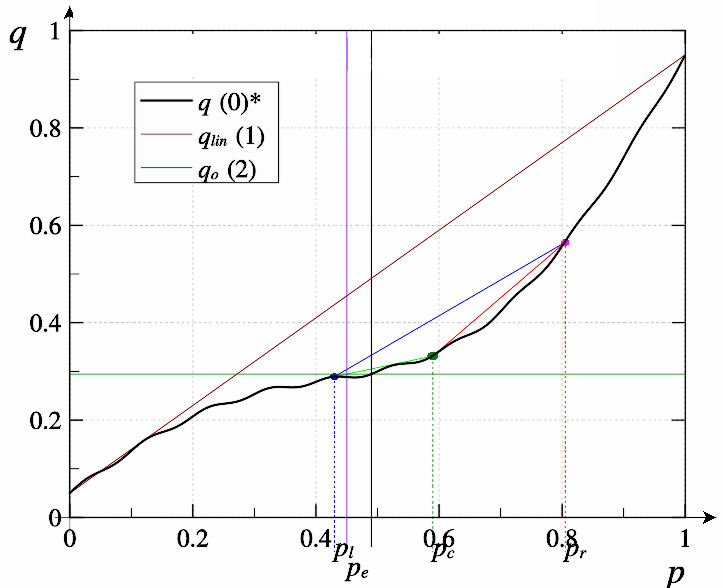
\includegraphics[width=49\TW]{p3/p/pq_sin-p_pq_po=049_xl.png}
    \hfill
    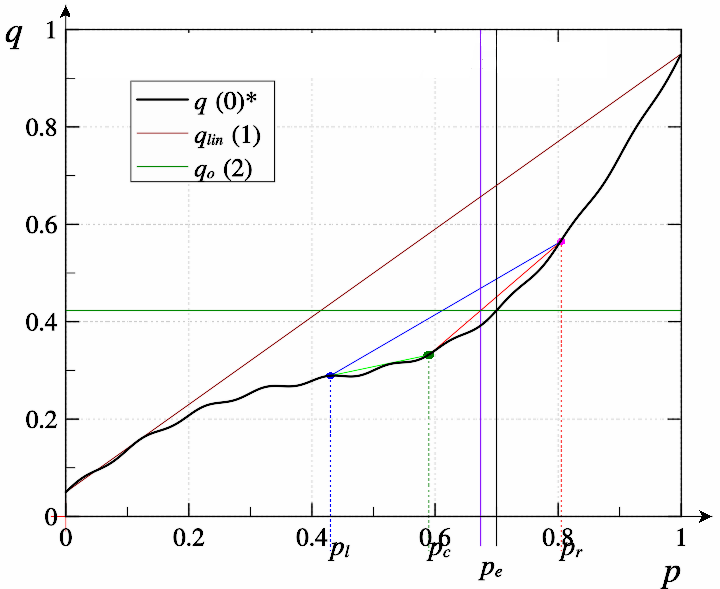
\includegraphics[width=49\TW]{p3/p/pq_sin-p_pq_po=070_xl.png}
  }
  \caption{Визначення точки $p_e$ методом $p_{eql}$ при $p_o \in [p_l, p_r]$}
  \label{atu:f:pq_4}
\end{figure}

У цьому, найсприятливішому випадку проводиться інтерполяція, а не екстраполяція
залежності $q(p)$, і досить вибрати ту ділянку, на якої гарантовано
відбувається перетин. При цьому значення всіх коефіцієнтів підкреслюють
впевненість агента в значенні $p_e$, що отримано:
%
\begin{equation}
  \tilde{p}_e
  =
  \begin{cases}
    \tilde{p}_{el}, & \tilde{q}_l < 0
    \\
    \tilde{p}_{er}, & \text{ otherwise}.
  \end{cases}
  ,
  c_\mathrm{su} = 1.0, \;  c_\mathrm{dist} = 0.5,  \;
  p_b =
  \begin{cases}
    -\tilde{p}_l, & \tilde{q}_l < 0
    \\
    \tilde{p}_r, & \text{ otherwise}.
  \end{cases}.
  \label{atu:eq:pr_e4}
\end{equation}

Останні випадки, за винятком точного збігу $q_o$ з $q_c$,
характеризуються меншою ``упевненістю'' в отриманому значенні $p_e$,
що відображається у коефіцієнтах
$c_\mathrm{su}$, $c_\mathrm{dist}$ та  $p_b$.
%
% У будь-якому з розглянутих випадків, має сенс ввести додаткове обмеження на
% значення $p_e$, так як через похибки вимірювання і моделювання воно може
% виявитися навіть поза діапазону $[p_{\min}, p_{\max}]$. З практичної
% точки зору досить добре зарекомендувало себе обмеження
% $\tilde {p}_r \in [2 \tilde{p}_l, 2 \tilde{p}_r]$.
% З урахуванням низького значення $S$ для
% агентів, які потрапили під таке обмеження, їх вплив на загальний результат буде
% мінімальним, так як нормальному перебігу процесу ідентифікації існує хоча б
% один агент з високим значенням $S$. Більш суворі обмеження досить рідко
% виправдовують себе, так як при цьому не використовуються екстраполяційні
% властивості агентів.
Описаний даними правилами спосіб визначення $p_e$ в подальшому будемо
означати як $p_{eql}$\label{atu:d:p_eql}.

% TODO: k_l ???

Розглянемо методи оцінювання величини $p_e$ для агентів, які використовують значення функції якості.
% Єдиний
% нерухомий агент, який використовує значення функції якості, ще більш марний (з
% точки зору синтезу системи ідентифікації), ніж один нерухомий агент, який
% використовує значення критерію.
% У найпростіших випадках можлива побудова системи ідентифікації з однією моделлю
% і, відповідно, одним пошуковим агентом.
% Пара агентів, що взаємодіє між собою, здатна оцінити градієнт функції якості,
% і, отже, забезпечити зміщення в потрібному напрямку.

Кожен пошуковий агент, визначаючи величину $q_{i}(t)$, і отримуючи $q_o(t)$,
обчислює безрозмірну функцію якості ідентифікації $F (q_o, q_i)$. Як
варіант, агент (або навіть вся керована частина системи ідентифікації) не має
безпосереднього доступу до критерію, і отримує власне значення~$F$.

Три сусідніх агента, які взаємодіють між собою, здатні не тільки оцінити градієнт
функції якості у власному околі, а й визначити наявність там
максимуму.

На відміну від методів, які використовують значення критерію безпосередньо, в
цьому випадку немає можливості обробляти кожну з пар точок $(p_l, p_c)$ і
$(p_c, p_r)$ незалежно. З трьох точок поблизу $M_{i}$ функція $F(p)$
апроксимується параболою, і абсциса її вершини задає шукане значення параметра.
Змістимо початок координат в точку
$(p_c, F_c)$. Тоді
% %
% \[
%   \tilde{p}_c = 0, \,
%   \tilde{p}_l = p_l - p_c, \,
%   \tilde{p}_r = p_r - p_c.
% \]
% %
% \[
%   \tilde{F}_c = 0, \,
%   \tilde{F}_l = F_l - F_c, \,
%   \tilde{F}_r = F_r - F_c.
% \]
% %
\[
  \left\{
    \begin{array}{l}
      a_2 \tilde{p}_l^2 + a_1 \tilde{p}_l  = \tilde{F}_l
      \\
      a_2 \tilde{p}_r^2 + a_1 \tilde{p}_r  = \tilde{F}_r
    \end{array}
  \right. .
\]
%
% \[
%   a_1 = \frac{\tilde{F}_r \tilde{p}_l^2 - \tilde{F}_l \tilde{p}_r^2 }
%              { \tilde{p}_l^2 \tilde{p}_r  - \tilde{p}_l \tilde{p}_r^2 }.
% \]
%
% \[
%   a_2 = - \frac{\tilde{F}_r \tilde{p}_l - \tilde{F}_l \tilde{p}_r }
%                { \tilde{p}_l^2 \tilde{p}_r  - \tilde{p}_l \tilde{p}_r^2 }.
% \]

\begin{equation}
   a_1 = \frac{\tilde{F}_r \tilde{p}_l^2 - \tilde{F}_l \tilde{p}_r^2 }
              { \tilde{p}_l^2 \tilde{p}_r  - \tilde{p}_l \tilde{p}_r^2 },
  \;
  a_2 = - \frac{\tilde{F}_r \tilde{p}_l - \tilde{F}_l \tilde{p}_r }
               { \tilde{p}_l^2 \tilde{p}_r  - \tilde{p}_l \tilde{p}_r^2 },
  \;
  \tilde{p}_e = - \frac{a_1}{2 a_2};
  \;
  p_e = p_c - \frac{a_1}{2 a_2}.
  \label{atu:eq:p_eFq}
\end{equation}

При цьому, якщо
$a_2 \ge 0$,
то потрібне обмеження $p_e$ та корекція $c_\mathrm{su}$ та $c_\mathrm{dist}$.
Визначення $p_e$ по (\ref{atu:eq:p_eFq}) будемо позначати як $p_{eFq}$.
Метод в найбільш сприятливому випадку, при
$p_o \in [p_l,p_r]$, представлено на рис.~\ref{atu:f:p_eFq_intra}.

\begin{figure}[htb!]
  \centerline{
    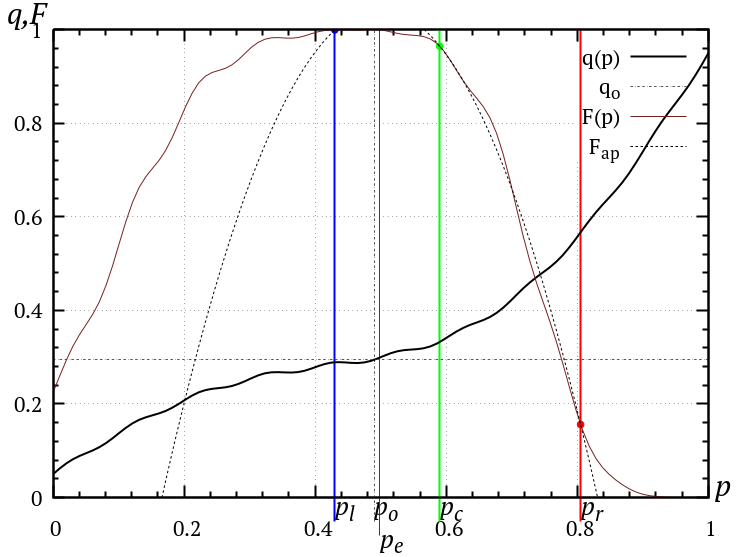
\includegraphics[width=49\TW]{p3/p/p_eFq/q_p_eFq_p49_xl.png}
    \hfill
    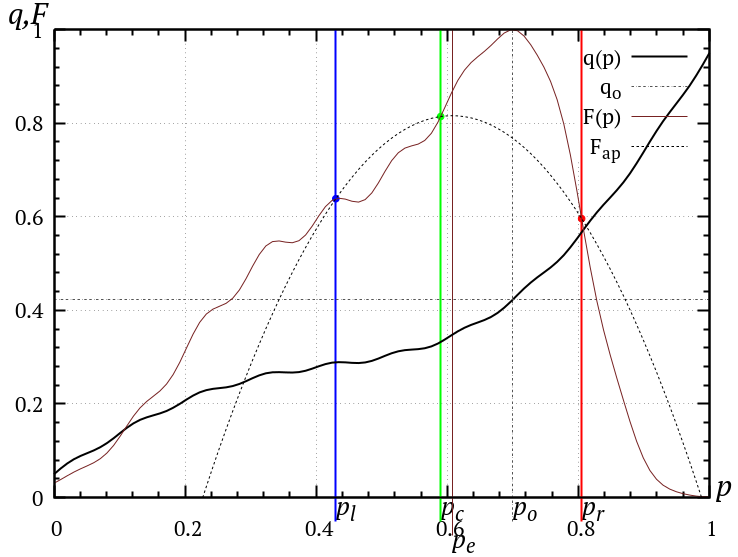
\includegraphics[width=49\TW]{p3/p/p_eFq/q_p_eFq_p70_xl.png}
  }
  \caption{Визначення точки $p_e$ методом $p_{eFq}$ при $p_o \in [p_l, p_r]$}
  \label{atu:f:p_eFq_intra}
\end{figure}

% Як і слід було очікувати, оцінка $p_e$ в цьому випадку цілком спроможна, не
% дивлячись на те, що в подібних умовах спостерігається різний рівень похибки
% ідентифікації.

Цій метод демонструє суттєву чутливість до значення $q_\gamma$.
Зайва чутливість призводить до того, що функція якості відмінна від нуля в
дуже вузькому діапазоні значень параметра, що призводить до практичної
безглуздості апроксимації, і неадекватними результатами
ідентифікації.
% Досить дивним є той факт, що при значному зменшенні чутливості похибка
% ідентифікації росте дуже слабо. В першу чергу це пов'язано з тим, що в цих
% умовах сама апроксимація кривої $F$ параболою стає більш точною. Для інших
% видів функції якості це не так. Більш того, наведені приклади розраховувалися
% за умови відсутності помилок вимірювання. При недостатній чутливості
% $F_l \approx F_c \approx F_r \approx 1$, і малі зміни $F$ приведуть до значної
% похибки ідентифікації.
В цілому, на підставі отриманих результатів, даний метод демонструє дещо
гірші результати, ніж $p_{eql}$.

Досить простим і маловитратними з точки зору обчислень є метод оцінювання $p_e$ методом
COG за значеннями функції якості:
%
\begin{equation}
  p_e =
  \frac{p_l F_l + p_c F_c + p_r F_r}{ F_r + F_c + F_r}  .
  \label{atu:eq:p_eFc}
\end{equation}

Умова обмеженості оцінки $p_e \in [p_l; p_r]$ в цьому випадку виконується
автоматично. Визначення $p_e$ по (\ref{atu:eq:p_eFc}) в подальшому будемо позначати $p_{eFc}$.

Для визначення працездатності і властивостей різних методів оцінювання $p_e$
в контрольованих умовах без урахування динаміки агентів, була обрана наступна
тестова задача: залежність $q (p)$ визначалася по (\ref{atu:eq:q_dem}),
$p_{\min}=20$, $p_{\max}=60$,
$q_{00}=7$, $c_\mathrm{lin}=-4.0$.
Початкове розташування агентів рівномірне, і штучно зафіксоване:
$p_l=30$, $p_c=40$,  $p_r=50$.

У першій серії обчислювальних експериментів значення параметра об'єкта $p_o$
змінювалося в діапазоні $[p_{\min}; p_{\max}]$ при фіксованій відстані
між агентами $A = p_c - p_l = p_r - p_c$. Це дозволило оцінити як
інтерполяційні (при $p_o \in [p_l, p_r]$), так і екстраполяційні можливості
методів. Так як частина методів при визначенні $p_e$ використовує значення
функції якості, то при проведенні експериментів величина $q_\gamma$ також
варіювалася.

На рис.~\ref{atu:f:qsl_pe_po_qg_all} представлені залежності помилок
ідентифікації для тестового завдання (\ref{atu:eq:q_dem}) при повному
комплекті нелінійних членів  трьома нерухомими
агентами трьома розглянутим методами визначення $p_e$.

\begin{figure}[htb!]
  \centerline{
    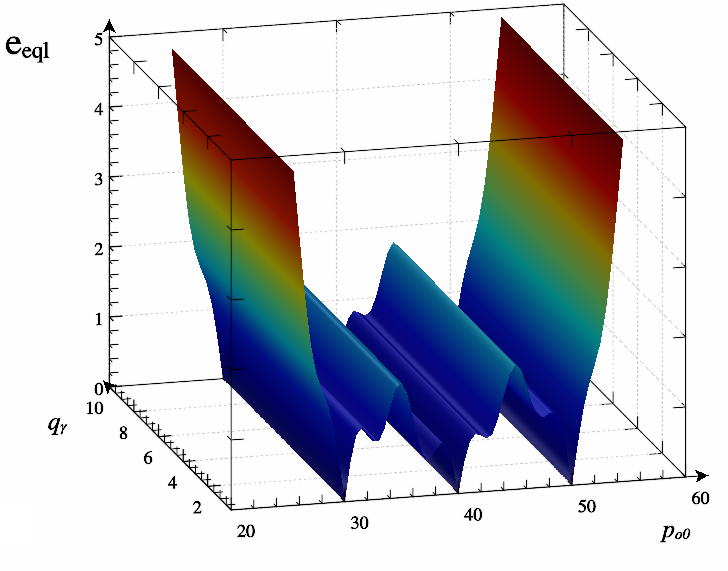
\includegraphics[width=0.32\textwidth]{p3/p/qls_pe-p_po_qg_eql_all_xl.png}
    \hfill
    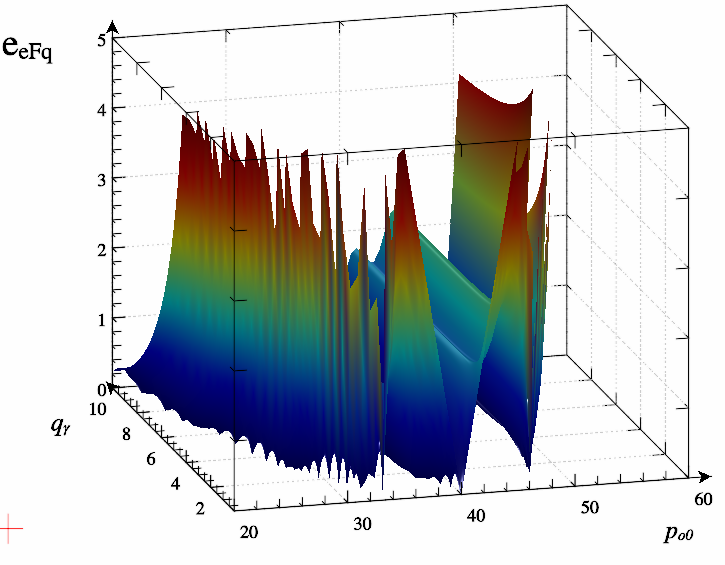
\includegraphics[width=0.32\textwidth]{p3/p/qls_pe-p_po_qg_eFq_all_xl.png}
    \hfill
    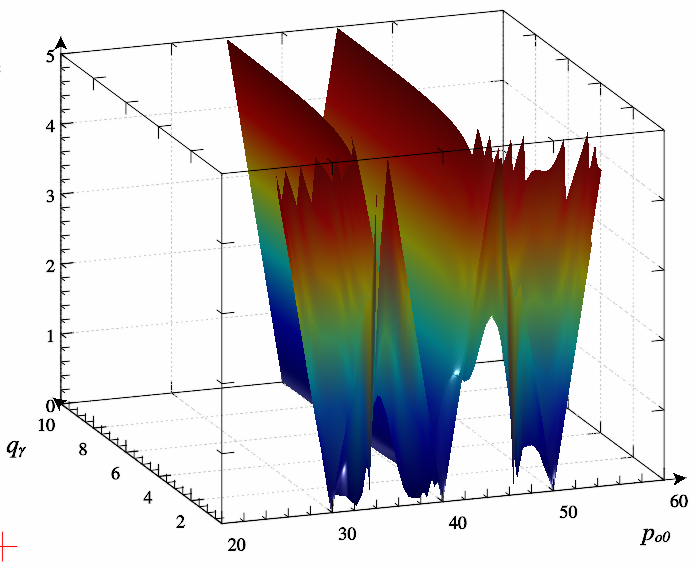
\includegraphics[width=0.32\textwidth]{p3/p/qls_pe-p_po_qg_eFc_all_xl.png}
  }
  \vspace{-1.5ex}
  \begin{center}
    ~ \hfill a \hfill\hfill b \hfill\hfill c \hfill ~
  \end{center}
  \vspace{-2.5ex}
  \caption{Залежності $e(p_o,q_\gamma)$ для методів $p_{eql}$ (a), $p_{eFq}$ (b), $p_{qFc}$ (c) при повному комплекті нелінійних членів}
  \label{atu:f:qsl_pe_po_qg_all}
\end{figure}

Метод $p_{eql}$ демонструє досить обмежену похибку ідентифікації при
$p_o \in [p_l; p_r]$, і досить швидке, але лінійно обмежене зростання похибки за
межами цього робочого діапазону. Метод $p_{eFq}$ має істотну залежність
від величини $q_\gamma$: малі значення призводять до суттєвого
зростання похибки, а з подальшим зростанням рівень похибки в межах робочого
діапазону приблизно одного порядку з похибкою в методі $p_{eql}$. При
цьому, за межами робочого діапазону спостерігається більш суттєве зростання
похибки. Метод $p_{qFc}$ демонструє прийнятні результати тільки в дуже
вузькому діапазоні значень $q_\gamma$, що ставить під серйозний сумнів
можливість застосування цього методу для реальних завдань, так як при цьому
немає можливості передбачити таке значення цього параметра, при якому метод буде
працездатний.

На рис.~\ref{atu:f:qsl_S_po_qg_all} представлені залежності
$S (p_o, q_\gamma)$
при тих же умовах, при яких було отримано рис.~\ref{atu:f:qsl_pe_po_qg_all}.
Використовувалося визначення (\ref{atu:eq:S3}), як
потенційно більш адекватне помилці ідентифікації.

\begin{figure}[htb!]
  \centerline{
    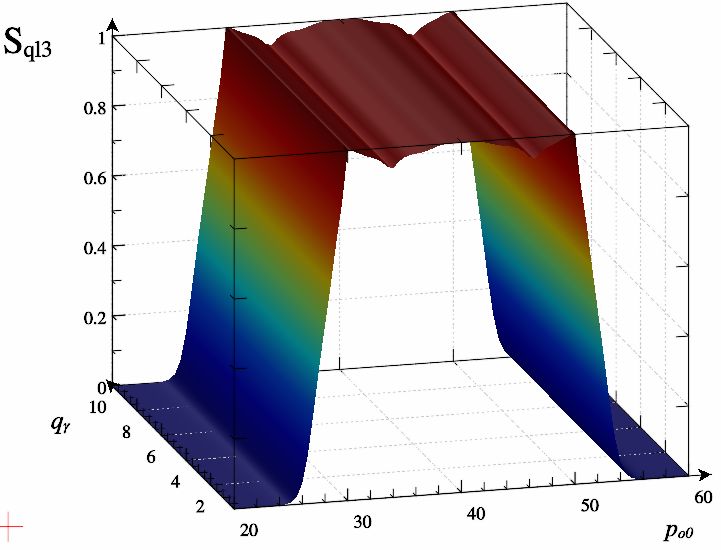
\includegraphics[width=0.32\textwidth]{p3/p/qls_pe-p_po_qg_Sql_all_xl.png}
    \hfill
    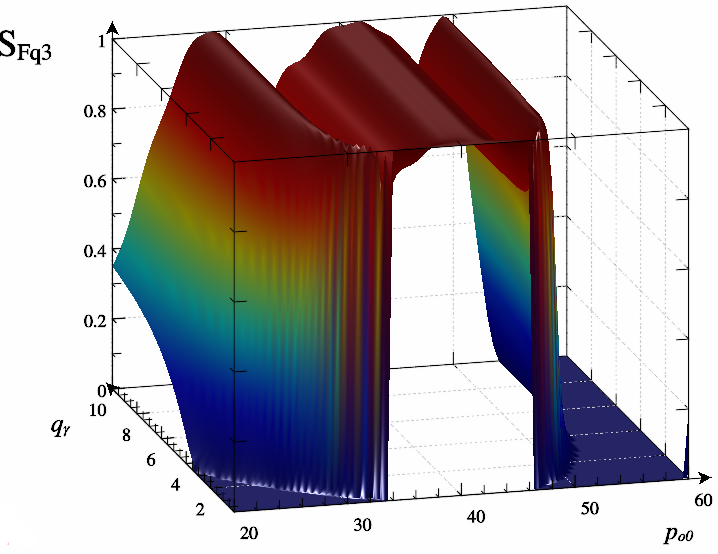
\includegraphics[width=0.32\textwidth]{p3/p/qls_pe-p_po_qg_SFq_all_xl.png}
    \hfill
    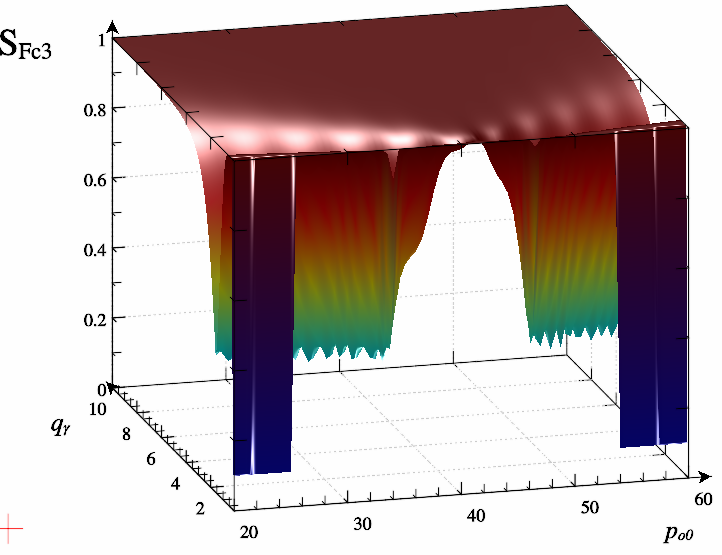
\includegraphics[width=0.32\textwidth]{p3/p/qls_pe-p_po_qg_SFc_all_xl.png}
  }
  \vspace{-1.5ex}
  \begin{center}
    ~ \hfill a \hfill\hfill b \hfill\hfill c \hfill ~
  \end{center}
  \vspace{-2.5ex}
  \caption{Залежності $S(p_o,q_\gamma)$ для методів $p_{eql}$ (a), $p_{eFq}$ (b), $p_{qFc}$(c)}
  \label{atu:f:qsl_S_po_qg_all}
\end{figure}

Для методу $p_{eql}$ близькі до одиниці значення $S$, як і планувалося,
спостерігаються в тих же областях, де і низький рівень похибки ідентифікації, в
першу чергу --- всередині робочого діапазону. При цьому, ця величина не
прямим відображення рівня похибки, так як це неможливо визначити за трьома точкам.
Метод $p_{eFq}$ також характеризується досить коректним видом цієї залежності,
включаючи низький рівень впевненості при підвищеній чутливості функції якості.
Навпаки, для методу $p_{eFc}$ графік показує, що для нього це визначення $ S$ не має сенсу.

У другій серії обчислювальних експериментів значення параметра об'єкта було
фіксованим $p_o = 39$, а відстань між агентами $A$ змінювалося від $0.1$
до $20$. При цьому, при $A <1$ точка $p_o$ перебувала за межами інтервалу
$[p_l, p_r]$, і становище $p_e$ визначалося за допомогою екстраполяції.
Значна частина цих графіків відображає протилежний випадок --- $p_O \in [p_l,p_r]$,
і значення $p_e$ визначається інтерполяцією на розширенні (з ростом $A$) діапазоні.
На рис.~\ref{atu:f:qsl_pe_A_qg_all} представлені поверхні залежностей помилок ідентифікації
при наявності всіх нелінійних членів.

\begin{figure}[htb!]
  \centerline{
    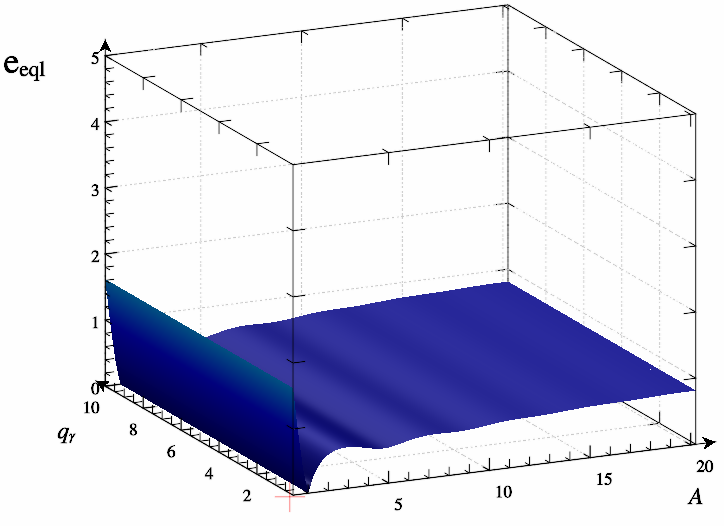
\includegraphics[width=0.32\textwidth]{p3/p/qls_pe-p_A_qg_eql_all_xl.png}
    \hfill
    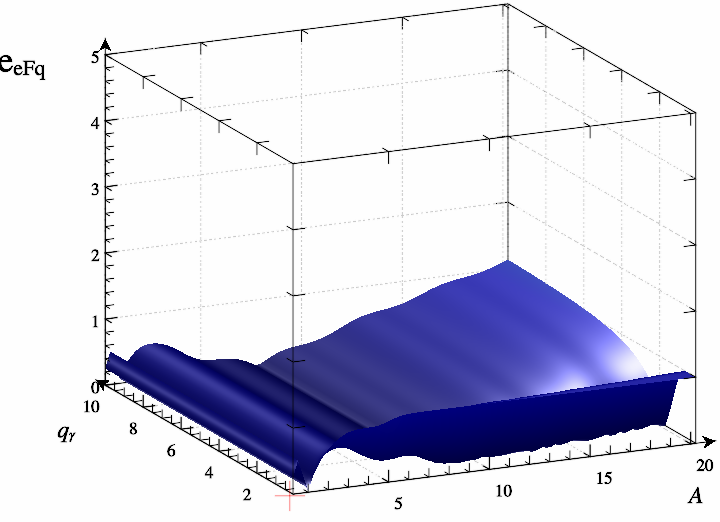
\includegraphics[width=0.32\textwidth]{p3/p/qls_pe-p_A_qg_eFq_all_xl.png}
    \hfill
    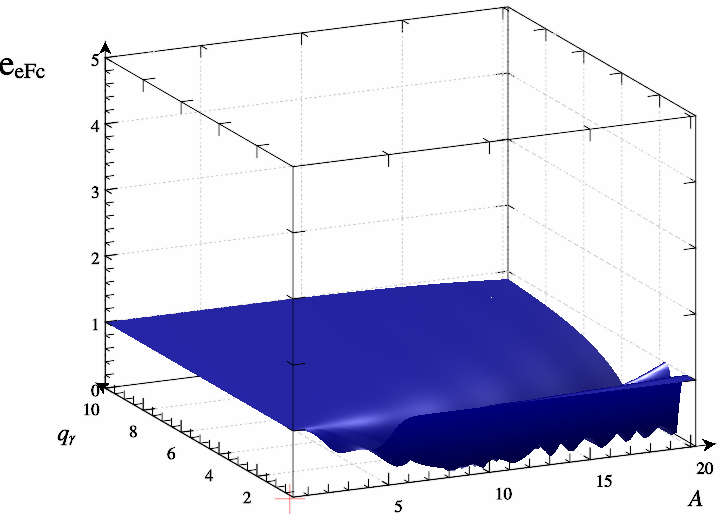
\includegraphics[width=0.32\textwidth]{p3/p/qls_pe-p_A_qg_eFc_all_xl.png}
  }
  \vspace{-1.5ex}
  \begin{center}
    ~ \hfill a \hfill\hfill b \hfill\hfill c \hfill ~
  \end{center}
  \vspace{-2.5ex}
  \caption{Залежності $e(A,q_\gamma)$ для методов $p_{eql}$ (a), $p_{eFq}$ (b), $p_{qFc}$ (c)}
  \label{atu:f:qsl_pe_A_qg_all}
\end{figure}

Для методу $p_{eql}$ форма цього графіка досить передбачувана --- немає
залежності від $q_\gamma$, на ділянці екстраполяції величина похибки
лінійно падає при $A \to p_c - p_o$. При подальшому зростанні $A$ похибка
помірно зростає, причому в цьому зростанні можна виділити дві ділянки. Перша
характеризується відносно різким зростанням похибки, що пов'язано зі збільшенням
впливу високочастотних нелінійних членів, друга --- досить плавним підйомом.
Графік, відповідний методу $p_{eFq}$ проявляє явну залежність похибки від
$q_\gamma$. Для широкого діапазону величини $ A $ існує досить вузька область
значень $q_\gamma$, при яких похибка мінімальна. Як надмірна, так і
недостатня чутливість функції якості призводить до зростання похибки.
Графік похибки для методу $p_{eFc}$ підкреслює обмежену придатність цього методу.

Таким чином, на підставі результатів моделювання можна зробити висновки про
можливість застосування розглянутих методів. Метод $p_{eFc}$ має гранично
обмежену придатність, у подальших дослідженнях в даній цей метод застосовуватися
не буде. При нормальному функціонуванні метод $p_{eql}$ забезпечує найкращі
результати. При цьому він складніше в реалізації, вимагає обробки ряду
особливих випадків. Метод $p_{eFq}$ демонструє результати, які можна
порівняти з методом $p_{eql}$, при цьому він простіший в реалізації. У тих
випадках, коли величина критерію самому агенту безпосередньо не відома, цей
метод, на відміну від методів, заснованих на апроксимації $q (p)$, зберігає
працездатність. Недоліком є істотна залежність від величини $q_\gamma$.
Методи $p_{eql}$ і $p_{qFq}$ дозволяє досягти меншої похибки
ідентифікації при зближенні пошукових агентів до $p_o$, за умови $p_o \in [p_l, p_r]$.


% {Динамика поисковых агентов}

Значення $p_e$, отримане пошуковим агентом, може використовуватися
безпосередньо і миттєво в якості значення параметрів для керованих моделей
тільки в тому випадку, якщо об'єкт, і отже моделі, не виявляють власної
динаміки, тобто є статичними. Ідентифікація статичних об'єктів не є ціллю
цієї роботи.

При моделюванні динаміки тіла без урахування обертання в механіці досить задати
всі сили, що діють на це тіло. Аналогічно, визначаючи пошукову динаміку агента
потрібно визначити еквівалент ``сил'', що викликають зсув параметрів моделей,
контрольованих агентом. При цьому задачу визначення динаміки можна спростити,
розділивши ``сили'' на дві групи. До першої входять сили, що призводять до ``руху''.
У другу входять сили опору, і замість розгляду самих сил досить
визначити правила динаміки, при цьому можливе використання правил, які не мають
прямого відображення на реальні фізичні системи.

Розглянемо способи визначення основних діючих сил.

$f_e$ --- ``сила тяжіння'' до локальної оцінки $p_e$, забезпечує зміщення
агента в напрямку цієї точки, і, отже, збільшення ``щільності'' агентів в
околі $p_o$. Найпростішим, очевидним, з прозорим фізичним змістом є
наступне визначення:
%
\begin{equation}
  f_e(t) = - k_e \left( p_c(t) - p_e(t) \right)  ,
  \label{atu:eq:f_e_lin}
\end{equation}
%
де $k_e$ --- коефіцієнт пропорційності, відповідний коефіцієнту жорсткості
умовної ``пружини'', що деформується при видаленні $p_c$ від $p_e$. Це
визначення досить універсальне, і має сенс при реалізації багатьох пошукових
тактик. Розглянуто інші способи визначення цієї сили, зокрема з фіксованою
абсолютною величиною та змінним напрямком, та гібридне визначення.
Загальним недоліком визначення сили $f_e$ за виразом (\ref{atu:eq:f_e_lin})
є той факт, що сила визначається тільки по локальним параметрами в окілі
агента. Більш того, ігнорується навіть локальне значення впевненості агента в
оцінці $p_e$. Тому має сенс використовувати додатковий множник у визначенні $f_e$,
наприклад $F$, $S$, $W$.

Наявність тільки сили $f_e$ призводить до того, що поведінка агентів буде
практично незалежною, і для реалізації властивостей ``ансамблю'' агентів
необхідне введення сил, що регламентують колективну поведінку. В першу чергу,
слід визначити силу $f_n$, яка визначає взаємодію агента з найближчими
сусідами. У досить загальному випадку цю силу можна визначити як
%
\begin{equation}
  f_n( p_r, p_c, p_l ) = f_{nr}(p_r-p_c) + f_{nl}(p_c-p_l).
  \label{atu:eq:f_n_gen}
\end{equation}

У разі лінійності і однакових визначень функцій $f_{nr}$ і $f_{nl}$ ця залежність набуває вигляду
%
\begin{equation}
  f_n = k_n ( p_r - 2 p_c + p_l ),
  \label{atu:eq:f_n_lin}
\end{equation}
%
де $k_n$ --- масштабний коефіцієнт, що відповідає коефіцієнту жорсткості
``пружин'', що з'єднують агенти. При цьому слід зазначити, що ця функція буде
приймати нульові значення при будь-якому рівномірному розподілі агентів.
Для уникання цього недоліку, та запобігання перетину траєкторій агентів,
можна використати таке визначення:
%
\begin{equation}
  f_n = k_n \left( \log\left( \frac{p_r-p_c}{p_{d0}} \right) -  \log\left( \frac{p_c-p_l}{p_{d0}}\right) \right),
  \label{atu:eq:f_n_log}
\end{equation}
%
де
$p_{d0}$ ---
базова відстань між агентами, звичайно дорівнює початкової відстані.

Також має сенс використовувати $f_c$ --- ``силу тяжіння'' до початкового значення параметра
($p_{c}(0)$) для даної моделі. У лінійній постановці ця сила визначається як
%
\begin{equation}
  f_c = -k_c (p_c - p_{c}(0)) ,
  \label{atu:eq:f_c}
\end{equation}
%
де $k_c$ --- коефіцієнт, що відповідає жорсткості ``пружини'',
що зв'язує агента з його початковим положенням.
Добре зарекомендували себе як нелінійні ``бар'єри'',
так і алгоритмічні методи, які утримують агента
більш-менш жорстко у виділеному йому діапазоні параметра.

З урахуванням вищевикладеного, визначимо суму всіх ``сил'',
що діють на пошуковий агент:
\begin{equation}
  f_t = f_c + f_n + f_e .
  \label{atu:eq:f_t}
\end{equation}


Можна використовувати різні способи визначення пошукової динаміки агента при
заданій силі. Наприклад, метод ``важкої кульки'':
\begin{equation}
  m \ddot{p}_c + \nu \dot{p}_c = f_t(t),
  \label{atu:eq:heavy_ball}
\end{equation}
%
де $m$ --- еквівалент маси кульки, $\nu$ --- коефіцієнт умовної в'язкості.

Також може використовуватися наближення динаміки тіла у в'язкій рідині, коли
вплив інерції дуже малий в порівнянні з в'язкістю, при цьому зміни параметрів
моделей (пошукових агентів) задаються наступним чином:
%
\begin{equation}
  \od{p_c}{t} = v_f f_t(t),
  \label{atu:eq:v_f}
\end{equation}
%
\noindent
де $f_t$ --- сума всіх діючих ``сил'',
$v_f = 1 / \nu$ --- коефіцієнт
пропорційності. Даний підхід, в порівнянні з попереднім, вимагає менших
обчислювальних витрат, і проявляє більшу стійкість. Більш слабкі пошукові
здібності компенсуються застосуванням множини агентів. Тому, в подальшому
викладі для багатомодельних систем буде застосовуватись саме цей підхід.
Існують методи адаптивно-пошукової ідентифікації, що визначають свої правила опису пошукової динаміки.


Розглянемо набір підходів визначення пошуковим координатором точки максимуму
функції якості, а отже --- значення ідентифікованого параметра.
%\cite{atu_st99,atu_jacs2015}.

З усього списку вихідних сигналів пошукових агентів координатор використовує
тільки необхідну йому підмножину. У якості координати може використовуватися як
$ p_c$, так і $p_e$.
У якості рівня важливості може використовуватися $F$, $S$, $W$.
В якості першого наближення $p_\mathrm{id}$ можна  використовувати
значення $p_c$ тієї моделі, для якої функція якості максимальна:
%
\begin{equation}
  p_{bcF}
  =
  p_{c,i};
  \quad
  i : F_i = \max{F_j}, \, j=0 \ldots N-1 .
  \label{atu:eq:p_bcF}
\end{equation}

Аналогічно визначаються залежності
$p_{bcS}$ та $p_{bcW}$.
Єдиною перевагою даного методу є простота реалізації. При цьому, ніяк не
використовуються апроксимуючи здатності агентів. Більш того, залежності
$p_{bcA} (t)$ схильні до стрибкоподібих змін в момент перемикання з однієї моделі
на іншу. Слід зазначити, що для методів, які використовують одну модель це
практично єдиний метод визначення
$p_\mathrm{id}(t)$.

Для того, що б використовувати апроксимуючи можливості кожного агента, у
визначенні (\ref{atu:eq:p_bcF}) замість $p_c$ можна використовувати $ p_e$.
Відповідні методи отримають позначення $p_{beS}$, $p_{beS} $ і $p_{beW}$.
Такі визначення, на відміну від (\ref{atu:eq:p_bcF}) дозволяють,
при досить хорошій апроксимації $q(p)$ принаймні одним кращим агентом,
реалізувати ідентифікацію для будь-якого
$p_o \in [p_{\min}, p_{\max}]$ при нерухомих агентах.

Наступний метод --- реалізація методу COG (Center of gravity, Такагі-Сугено),
який використовується при дефазифікації систем нечіткої логіки для всього
ансамблю:
%
\begin{equation}
  p_{gcF}
  =
  \frac{\sum\limits_{i=0}^{N-1} F_{i} p_{i}}
       {\sum\limits_{i=0}^{N-1} F_{i} }
  .
  \label{atu:eq:p_gcF}
\end{equation}
%
Аналогічно визначаються методи
$p_{gcS}$,
$p_{gcW}$,
$p_{geF}$,
$p_{geS}$ та
$p_{geW}$.


Наступний підхід призначений зменшити залежність першого від впливу локальних
екстремумів і границь. В цьому випадку визначається модель $M_{i_{m}}$ ($M_{c}$) з
максимальним значенням $F$, а в оцінці використовується тільки найближчий
окіл цієї моделі:
%
\begin{equation}
  p_{leF}
  =
  \frac{ F_{l} p_{l} + F_{c} p_{c} + F_{r} p_{r} }
       { F_{l}       + F_{c}       + F_{r}       }
  .
  \label{atu:eq:p_lcFl}
\end{equation}
%
Аналогічно визначаються методи
$p_{lcS}$,
$p_{lcW}$,
$p_{leF}$,
$p_{leS}$ та
$p_{leW}$.


Так само в околі кращого агента можна використовувати інтерполяцію по
$F$, аналогічно (\ref{atu:eq:p_eFq}). В позначенні таких методів будемо
використовувати перший символ ``q'', наприклад $p_{qeF}$.

Похибки ідентифікації в просторі параметрів для розглянутих підходів позначимо відповідно:
%
\begin{equation}
  e_{gcF} = p_{gcF} - p_o,
  \quad
  e_{leF} = p_{leF} - p_o,
  \quad
  \ldots
  \quad
  e_{leW} = p_{leW} - p_o.
  \label{atu:eq:e_xx}
\end{equation}
%

У даній роботі розглядається набір методів ідентифікації нелінійних динамічних
систем. При цьому, більшість з них мають загальні властивості, і система
ідентифікації в цілому складається з ``набору'' модулів і алгоритмів,
комбінація яких дозволяє вибрати конкретний метод, що підходить для даної
задачі.
Пропонується до використання наступна система позначень, яка послідовно визначає
компоненти системи ідентифікації, починаючи з агентів.

\begin{enumerate}

  \item
  Перший символ (``F'', ``q'', ``x'' ) визначає,
  яка величина використовується кожним агентом для визначення $p_e$.

  \item
    Другий символ (``l'' --- linear, ``q'' --- quadratic \ldots ) 
    задає спосіб визначення величини $p_e$ одним агентом.

  \item
  Третій символ визначає локальну пошукову геометрію, найчастіше --- кількість
    агентів в в пошуковій групі, наприклад: ``2'' --- пошукова пара, ``3'' --- триплет.

  \item
    Четвертий символ (``z'' --- zero, ``r'' --- real \ldots),
    описує поведінку додаткових моделей, які розташовані на границі:

  \item
    П'ятий символ (``c'' --- const, ``l'' --- linear \ldots )
    позначає вибрану залежність для величини $f_e$ (або
    аналогічної величини, якщо $f_e$ безпосередньо не використовується).

  \item
    Шостий символ (``o'' --- one, ``F'', ``S'', ``W'') визначає множник,
    використовуваний для величини $f_e$ при визначенні динаміки об'єкта.

  \item
   Сьомий символ (``z'' --- zero, ``v'' --- viscous \ldots)
    вказує, яким чином величина $f_t$ (або її еквівалент) впливає на динаміку агента.

  \item
   Восьмий (``n'' --- none, ``t'' --- triangle \ldots ) символ дозволяє вказати,
    який додатковий пошуковий рух реалізує агент.

  \item
    Дев'ятий символ задає спосіб визначення ідентифікованого параметра по всьому ансамблю:
    \begin{description}

      \item[b]  --- ``best''
        --- вибирається найкращий агент без подальшої обробки;

      \item[g]  --- ``global COG'' ---
        метод ``Center of Gravity'' по всьому ансамблю~(\ref{atu:eq:p_gcF});

      \item[l] --- ``local COG'' ---
        метод ``Center of Gravity'' по околі кращого агента;

      \item[q] ---
        інтерполяція другого порядку в околі кращого агента~(\ref{atu:eq:p_eFq}).

    \end{description}

  \item
    Десятий символ (``c'', ``e'') визначає, який з вихідних сигналів пошукового агента використовується.

  \item
    Одинадцятий символ (``F'', ``S'', ``W'') вказує,
    яка величина використовується для визначення ваги кожного агента.


\end{enumerate}
%
Для позначення підмножин методів замість позначення елемента використовується символ ``A'' --- ``any''.
Якщо виникає потреба вказати конкретний вид критерію, то в кінець даного
позначення, через точку, додається позначення критерію.

Приклад позначень:
``Fc3zlovngcW.$q_{x^2}$''
--- метод, агенти якого для оцінювання величини $p_e$ використовують функцію
якості і квадратичну апроксимацію за даними кожних трьох сусідніх агентів, 2
псевдомоделі на границі, залежність $f_e (p_e-p_c)$ --- лінійна, ``в'язка''
динаміка, одиничний коефіцієнт при цій силі, ``global COG'' для результуючого
значення параметра по значенням $p_c$ і $W$, критерій
``$q_{x^2}$''.


Якість ідентифікації для процесу в цілому задається мірою:
%
\[
  \overline{e} = \mu( p_o(t), p_\mathrm{id}(t) ),
  \quad
  t \in [0;T].
\]

Конкретний вид міри визначається задачею. Якщо в конкретній постановці
важливо знати максимальне відхилення ідентифікованого параметра моделі від
об'єкта, то має сенс вибрати міру $C[0; T]$ або ж $ R_{\infty}^n$ для
дискретного представлення:
%
\begin{equation}
  \overline{e_c}(p_o(t),p_\mathrm{id}(t))
  =
  \max \big| p_o(t)-p_\mathrm{id}(t) \big|,
  \quad
  t \in [0;T].
  \label{atu:eq:e_c}
\end{equation}

Більш поширеним є випадок, коли інтерес представляє не максимальне значення
$|e(t)|$, а якийсь варіант усереднення цієї величини, наприклад
%
\begin{equation}
  \overline{e_2}(p_o(t),p_\mathrm{id}(t))
  =
  \sqrt{ \frac{1}{T} \int\limits_{0}^{T} \big( p_o(t)-p_\mathrm{id}(t) \big)^2 \, \mathrm{d}t },
  \label{atu:eq:e_2}
\end{equation}

Саме значення як похибки ідентифікації, так і відповідної міри ---
величина розмірна, і в такому вигляді не придатна для незалежного від
конкретної ситуації оцінювання якості роботи методу. Розглянемо можливі
величини, що дають можливість привести похибку ідентифікації до безрозмірного
вигляду. В першу чергу, припустимо, що взагалі не проводимо ніякої
ідентифікації, а в якості значення параметра використовуємо або геометричний
центр $p_{00}$ множини $\mathcal{P}$, або, якщо це з небудь-якої причини
відомо, точку з максимальним значенням щільності ймовірності. Тоді позначимо
%
\begin{equation}
  \overline{e}_{00}
  =
  \overline{e}(p_o(t),p_{00})
  \label{atu:eq:e_00}
\end{equation}

Відносні похибки для відповідних абсолютних~(\ref{atu:eq:e_xx})
тоді будуть визначені в такий спосіб:
%
\begin{equation}
  \overline{e}_{rbcF} = \frac{\overline{e}_{bcF}}{\overline{e}_{00}}, \;
  \overline{e}_{rleS} = \frac{\overline{e}_{leS}}{\overline{e}_{00}}, \;
  \overline{e}_{rgeW} = \frac{\overline{e}_{geW}}{\overline{e}_{00}},
  \ldots
  \overline{e}_{rqeF} = \frac{\overline{e}_{qeF}}{\overline{e}_{00}}.
  \label{atu:eq:e_rxx}
\end{equation}

Близькість цих величин до одиниці свідчить про те, що даний метод ідентифікації
в розглянутих умовах марний. Більш того, при серйозних порушеннях в процесі
пошуку, наприклад при втраті стійкості, ці величини можуть і перевершувати
одиницю.
Для врахування вкладу динаміки агентів запропоновано проводити нормалізацію
на початкову відстань проміж ними.

% Дослідження працездатності та властивостей методів на тестових завданнях.

Для оцінювання можливостей системи ідентифікації відстежувати як гладкі, так і
стрибкоподібні зміни параметрів, пропонується для кожної тестової системи, якщо
це можливо, проводити моделювання процесів ідентифікації за умовами:
%
\begin{equation}
  p_o(t) = p_0 +  U_{p} \sign \sin( \omega_{p} t ),
  \label{atu:eq:po_t_sign}
\end{equation}
%
%
\begin{equation}
  p_o(t) = p_0 +  U_{p} \sin( \omega_{p} t ).
  \label{atu:eq:po_t_sin}
\end{equation}
%
\begin{equation}
  p_o(t) = p_0 +  U_{p} \frac{t}{T}.
  \label{atu:eq:po_t_ramp}
\end{equation}


Розглянемо конфігурації рівноважного стану пошукових агентів при застосуванні
різних пошукових тактик з числа розглянутих. Для даного завдання немає
необхідності розглядати поведінку координатора пошуку, тому три правих символу
класифікації тут значення не мають.
Використовувалося 5 пошукових агентів: $A_0 \ldots A_4$, початкові
координати яких ($p_{ci,0}$) були розподілені по пошуковому діапазони
рівномірно. Залежність $p_o (t)$ задана як (\ref{atu:eq:po_t_ramp}), при
цьому величини $p_o$ і $U_p$ обрані таки чином, щоб покрити весь робочий
діапазон: $p_0 = p_{c0,0} = 20$, $U_p = p_{c4,0} - p_{c0,0} = 40$.


На рис.~\ref{atu:f:qls_ramp_Fq3rlovnAAF} наведені результати моделювання при використанні групи методів
``Fq3rlovnAAF''. Слід зазначити, що практично у всьому діапазоні об'єкт
``супроводжується'' двома агентами, і тільки в області ``передачі'' наступній
групи це число зростає до трьох. Слід зазначити відсутність коливань. До
негативних явищ можна буде отнести те, що віддалені агенти притискаються до
кордону виділеної їм області, що обумовлено використанням одиничного множника у
визначенні $f_e$. Також необхідно відзначити збільшення
``дистанції супроводу'' в околі точки $p_o = 40$, $t = 10$.

\begin{figure}[htb!]
    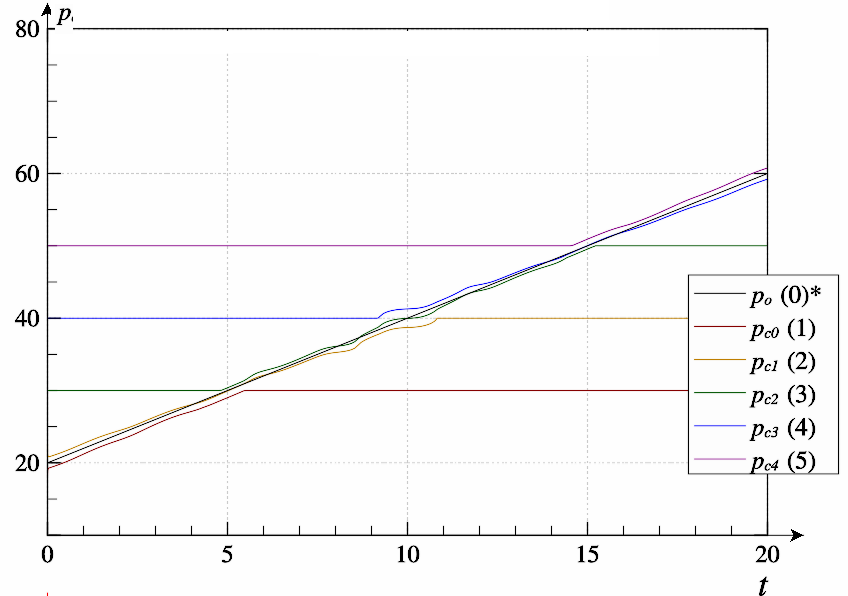
\includegraphics[width=0.48\textwidth]{p3/p/ramp/qls-p_t_pi_Fq3rlovnAAF_ramp_xl.png} \hfill
    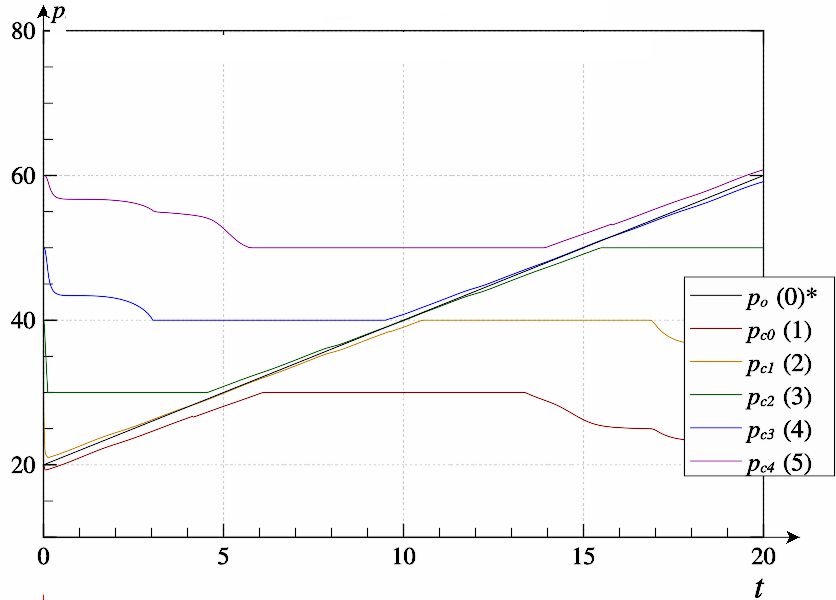
\includegraphics[width=0.48\textwidth]{p3/p/ramp/qls-p_t_pi_ql3rlWvnAAF_ramp_xl.png}
  \\
  \parbox[t]{0.48\textwidth} {
    \caption{Рівноважні конфігурації агентів при використанні групи методів  Fq3rlovnAAF}
    \label{atu:f:qls_ramp_Fq3rlovnAAF}
  }
  \hfill
  \parbox[t]{0.48\textwidth} {
    \caption{Рівноважні конфігурації агентів при використанні групи методів ql3rlWvnAAF}
    \label{atu:f:qls_ramp_ql3rlWvnAAF}
  }
\end{figure}

На рис.~\ref{atu:f:qls_ramp_ql3rlWvnAAF} наведені результати моделювання при використанні групи методів
``ql3rlWvnAAF''.
Відмінність проявляється в меншому зміщенні віддалених агентів, що, без
істотної зміни точності, повинно призводити до зменшення часу реакції системи на
стрибкоподібну зміну параметра.
Також було досліджено рівноважні конфігурації агентів для
груп методів
``Fq3rlFvnAAF'',
``Fq3rlSvnAAF'',
``Fq3rlWvnAAF'',
``ql3rlovnAAF'',
``ql3rlFvnAAF'' та
``ql3rlSvnAAF''.
Встановлено, що в тих випадках, коли для оцінювання $p_e$ використовується
метод $p_{eFq}$, то не має сенсу в якості множника при $f_e$
використовувати $S$ або $W$. Найкращим вибором в цих умовах буде
використання значення функції якості~$F$. До того ж, що підтверджується і
результатами дослідження якості апроксимації $q(p)$, використання методів,
які використовують кусково-лінійну апроксимацію, найбільш прийнятно. У цих
умовах стає виправданим в якості вищезгаданого множника використовувати~$S$
і~$W$, причому останній варіант видається більш виправданим.


Рівноважні конфігурації агентів, які були представлені вище, дають інформацію тільки про
потенційні властивості систем ідентифікації. В першу чергу, якість визначається
похибкою ідентифікації. В якості тестової задачі
використовується~(\ref{atu:eq:q_dem}) з усіма нелінійними членами. При цьому для кожного методу
проводилася серія обчислювальних експериментів з різним значенням~$p_o$. Інші
параметри як системи ідентифікації, так і умови експериментів вибиралися таким
чином, щоб з одного боку, забезпечити квазістаціонарність в кінці експерименту, а
з іншого --- досягти хорошої швидкості ідентифікації, для надання можливості
досліджувати динамічні властивості без переналаштовування параметрів.
Представлення отриманих результатів ускладнюється тим, що з урахуванням тільки
основних розглянутих елементів в класифікації, виходить 192 можливих метода.
Тому на одному графіку можна відобразити залежності для восьми методів.
У авторефераті наведено дві найкращі групи з~24.

Як перший приклад розглянемо групу методів
``Fq3rlFvnAAF'' (рис.~\ref{atu:f:Fq3rlFvnAAF_scan}).
На рис.~\ref{atu:f:ql3rlWvnAAW_scan} наведено залежності для групи методів ql3rlWvnAAW.

\begin{figure}[htb!]
   \begin{center}
     ~ \hfill
    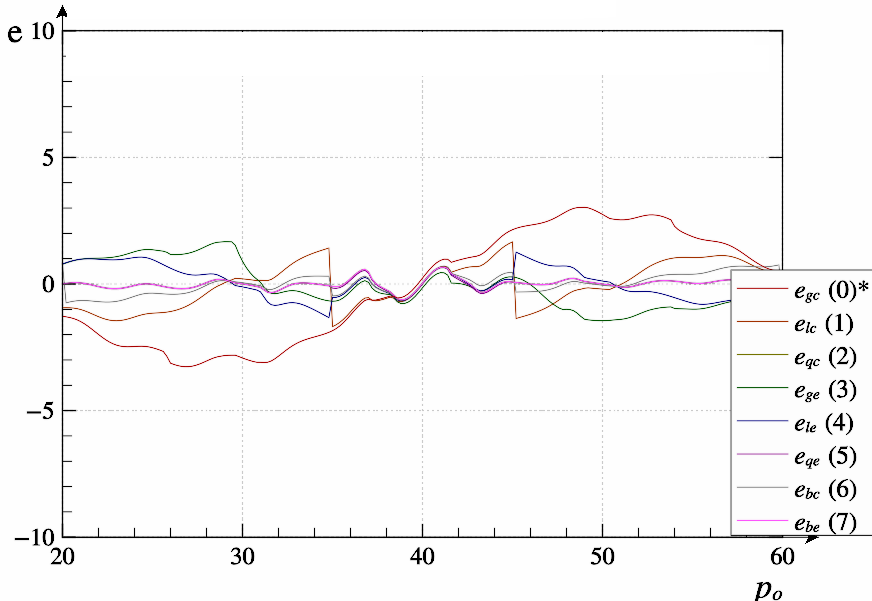
\includegraphics[width=0.48\textwidth]{p3/p/scan/qls-p_p_e_Fq3rlFvnAAF_scan_xl.png}
     \hfill
    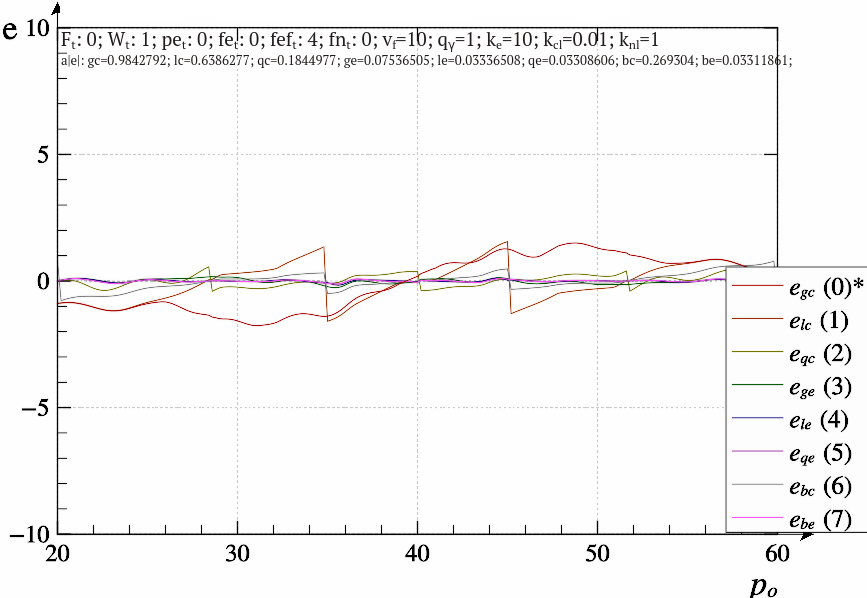
\includegraphics[width=0.48\textwidth]{p3/p/scan/qls-p_p_e_ql3rlWvnAAW_scan_xl.png}
     \hfill ~
   \end{center}
  \parbox[t]{0.48\textwidth} {
    \caption{Залежності $e (p_o)$ для групи методів Fq3rlFvnAAF в квазістаціонарному випадку}
    \label{atu:f:Fq3rlFvnAAF_scan}
  } \hfill
  \parbox[t]{0.48\textwidth} {
    \caption{Залежності $e (p_o)$ для групи методів ql3rlWvnAAW в квазістаціонарному випадку}
    \label{atu:f:ql3rlWvnAAW_scan}
  }
\end{figure}

Істотною відмінністю методів ``ql3r\ldots'' є менший загальний рівень
помилок, а також відсутність нахиленої ділянки залежності $e (p_o)$ при
$p_o \approx 40$. В околі цієї точки похідна приймає близьке до нуля значення, і
методи ``Fq3r\ldots'' не забезпечують належної чутливості в цій області, що
призводить до зростання похибки ідентифікації.
Таким чином, в квазістаціонарному випадку існує достатній набір працездатних
методів. При наявності можливості, слід використовувати методи, які
використовують величину критерію, на рівні координатора --- $p_e$, і
наприклад, $W$. Вибір інших елементів класифікації повинен проводитися
виходячи з інших умов, наприклад, вимог до динамічних характеристик системи
ідентифікації.

Для дослідження динамічних властивостей розглянутих методів ідентифікації без
прив'язки до конкретного об'єкта, будемо вважати, що для тестової задачі
характерний час стабілізації критерію значно менший характерних часів процесів
пошуку.
Таким чином, будемо розглядати тестове завдання~(\ref{atu:eq:q_dem}),
заданий повний набір коефіцієнтів, а динаміка параметра описується меандром~(\ref{atu:eq:po_t_sign}).
При цьому для аналізу буде використовуватися тільки один фронт~$p_o(t)$.

Для оцінки динамічних властивостей методів ідентифікації необхідна природна
одиниця часу, яка визначається самою системою ідентифікації.
%В якості такої
%одиниці пропонується використовувати час, за яке агент перетинає всю свою
%робочу смугу, за умови, що $f_e$ зберігає максимальне можливе значення під
%час руху, іншими силами нехтуємо. Тоді цей час визначається наступним чином:
Визначимо цей час  наступним чином:
%
\begin{equation}
  t_{ua} = \frac{p_r - p_l}{ v_f k_e (p_r - p_l)} = \frac{1}{v_f k_e}.
  \label{atu:eq:t_ua}
\end{equation}
%
У розглянутих прикладах $t_{ua} = 0.01$.

Динаміка агентів і значень ідентифікованих параметрів для групи методів
``Fq3rlovnAAW'' і вищевказаних умовах приведена на рис.~\ref{atu:f:Fq3rlovnAAW_sign}.

\begin{figure}[htb!]
  \centerline{
    ~ \hfill
    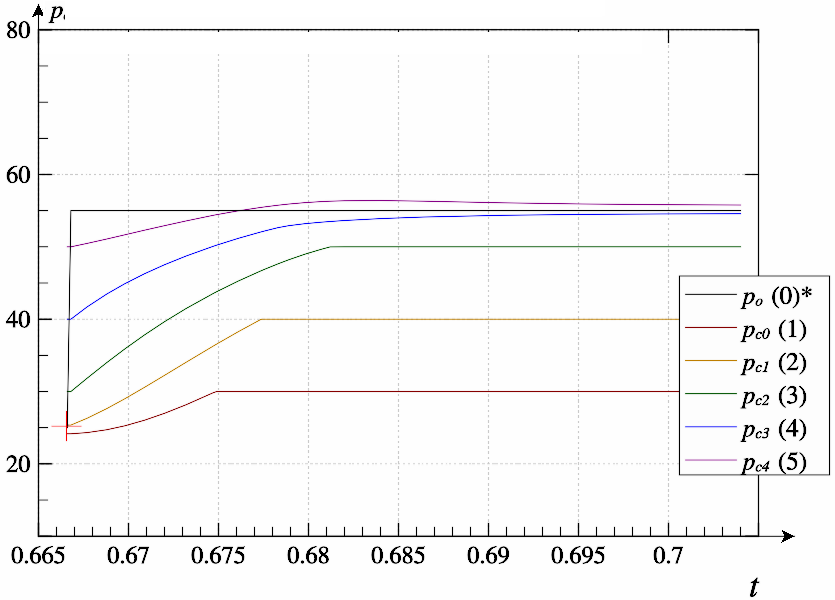
\includegraphics[width=0.45\textwidth]{p3/p/sign/qls-p_t_pi_m_Fq3rlovnAAW_sign_xl.png}
    \hfill
    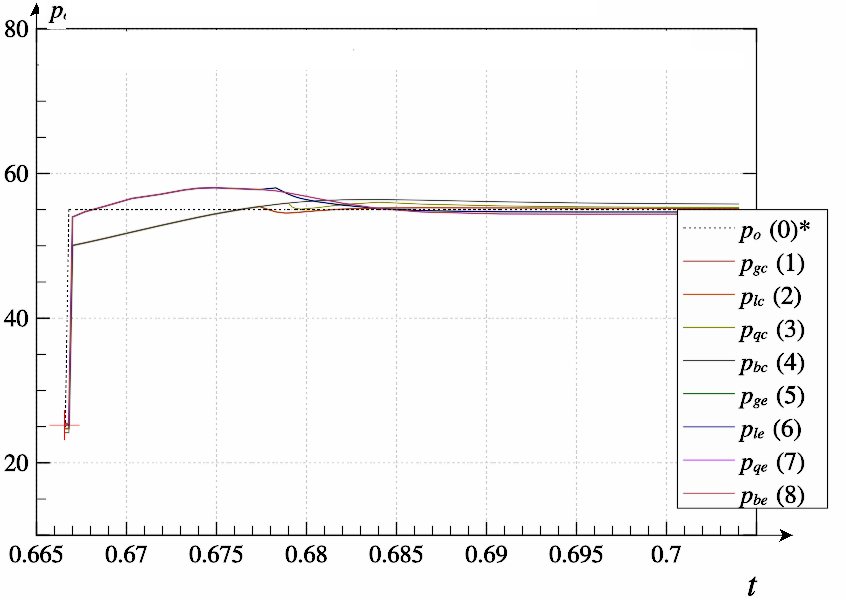
\includegraphics[width=0.45\textwidth]{p3/p/sign/qls-p_t_p_m_Fq3rlovnAAW_sign_xl.png}
    \hfill ~
  }
  \vspace{-1.5ex}
  \begin{center}
    ~ \hfill a \hfill\hfill b  \hfill ~
  \end{center}
  \vspace{-2.5ex}
  \caption{Динаміка реакції агентів (a) та $p_\mathrm{id}$ (b) на стрибок параметру для групи методів ``Fq3rlovnAAW''}
  \label{atu:f:Fq3rlovnAAW_sign}
\end{figure}

Ця група методів характеризується одиничним множником у визначенні $f_e$, що,
з одного боку, дає можливість агентам зміщуватися з максимальною швидкістю, з
іншого --- призводить до того, що ``далекі'' агенти зміщуються сильно,
займаючи місце поблизу границі свого робочого діапазону. Як наслідок --- після
стрибка параметра поблизу положення, відповідного новому значенню, немає
досить близько розташованого агента, що збільшує час реакції системи.

Використання  групи методів ``ql3rlWvnAAW'',
приводить до більш сприятливої до ідентифікації динамічних систем ситуації
(рис.~\ref{atu:f:ql3rlWvnAAW_sign}).

\begin{figure}[htb!]
  \centerline{
    ~ \hfill
    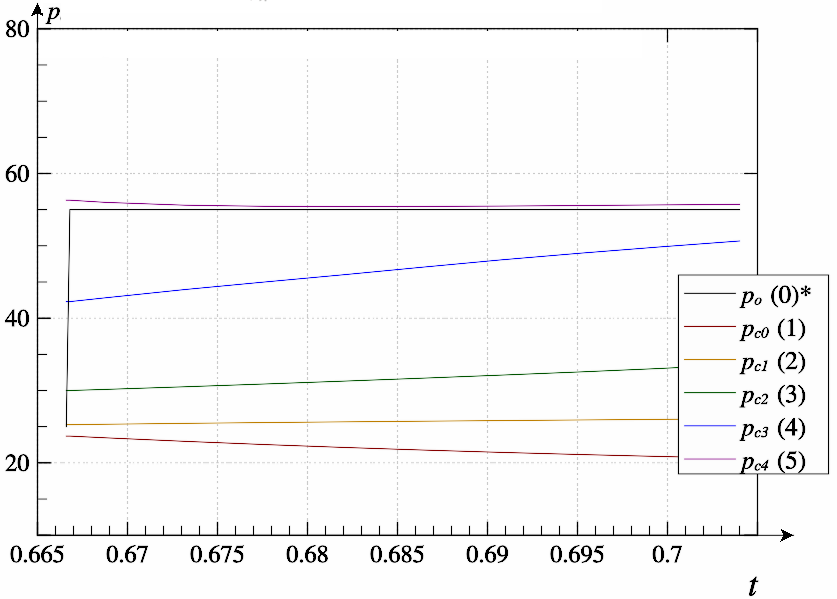
\includegraphics[width=0.45\textwidth]{p3/p/sign/qls-p_t_pi_m_ql3rlWvnAAW_sign_xl.png}
    \hfill
    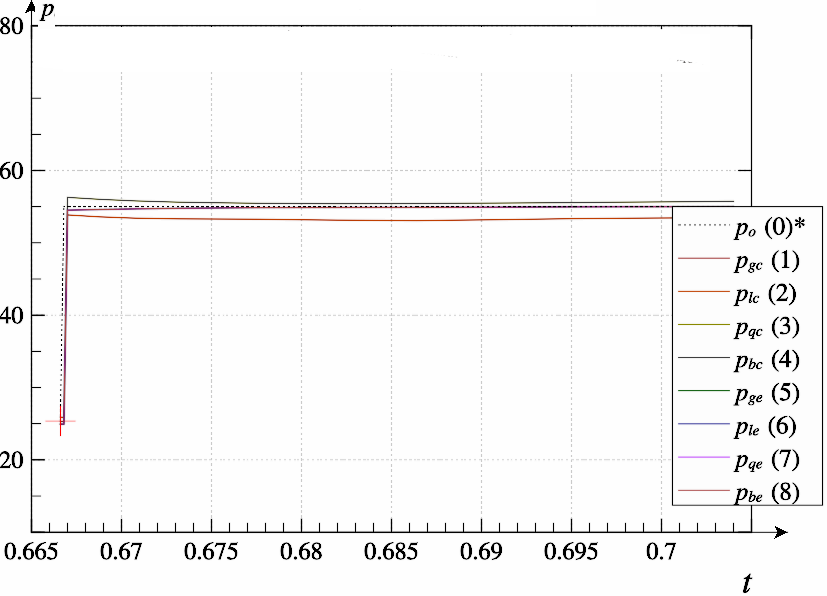
\includegraphics[width=0.45\textwidth]{p3/p/sign/qls-p_t_p_m_ql3rlWvnAAW_sign_xl.png}
    \hfill ~
  }
  \vspace{-1.5ex}
  \begin{center}
    ~ \hfill a \hfill\hfill b  \hfill ~
  \end{center}
  \vspace{-2.5ex}
  \caption{Динамика реакції агентів та $p_\mathrm{id}$ на стрибок параметру для групи методів ``ql3rlWvnAAW''}
  \label{atu:f:ql3rlWvnAAW_sign}
\end{figure}

Як вже було зазначено, використання у визначенні $f_e$ значень $F$, $W$,
не дозволяє ``віддаленим'' агентам зміщуватися занадто сильно. Така відмінність
призводить до того, що всі розглянуті методи дуже швидко (у порівнянні з $t_{ua}$)
стабілізуються в околі свого кінцевого значення.
% Відмінність
% проявляється лише в тому, яке це значення. Методи, які використовують значення
% $p_c$ агента, характеризуються дещо більшими похибками
% ідентифікації. З іншого боку, методи, які використовують $p_e$ агентів,
% характеризуються практично однаковою низькою похибкою ідентифікації.
%
Для даної тестової задачі принципових відмінностей між групами методів
``ql3rlFvnAAW'', ``ql3rlSvnAAW'' і ``ql3rlWvnAAW'' не спостерігається. Для
реальних завдань ідентифікації відмінності можуть бути істотнішими.



\medskip
\textbf{У третьому розділі}
розглядається розроблене програмне
забезпечення
для моделювання
поведінки  нелінійних,
у тому числі хаотичних динамічних систем.
Програма ``qontrol'' була створена для моделювання динаміки
нелінійних систем та проведення аналізу.

Мова програмування --- C++,
графічний інтерфейс реалізований за допомогою
бібліотек Qt та mathGL.
Розроблено ієрархію класів для
моделювання різноманітних елементів,
у тому числі суттєво нелінійних.

Також було створено спеціалізоване
програмне забезпечення для мікроконтролерів,
для забезпечення взаємодії
з реальними динамічними системами.


\textbf{У четвертому розділі}
розглянуте практичне застосування розроблених методів при моделюванні
процесів ідентифікації ряду систем хаотичної динаміки,
ак відомих, так і тих, які розглянуті вперше.

У якості першої ідентифікованої хаотичної системи розглянемо класичну систему
Лоренца, динаміка якої описується системою рівнянь:
%
\begin{equation}
\begin{cases}
  \dot{x} = \sigma (y-x ) , \\
  \dot{y} = x (r-z) - y , \\
  \dot{z} = x y - b z .
\end{cases}
\label{atu:eq:lor}
\end{equation}

Найціннішим з точки зору ідентифікації є параметр $r$, що визначає як
енергетичний стан системи, так і вид динаміки системи. Це підтверджують і
фізичні обґрунтування. Для визначеності задамо інші параметри наступним
класичним чином: $b = 8/3$, $\sigma = 10$, якщо не буде явно
зазначено протилежне.

При малих значеннях параметра $r$ система демонструє затухаючі коливання.
Далі, в широкому діапазоні значення параметра $r$ система проявляє хаотичну
динаміку. Крім цього, спектр даної системи в хаотичному режимі досить широкий
(рис.~\ref{atu:f:lor_attractor_phase_chaos28}) і не має домінуючих
частот, що не характерно для багатьох систем динамічного хаосу.
При подальшому зростанні параметра $r$ динаміка системи стає
складно-періодичною, з явно вираженим лінійчатим спектром.

\begin{figure}[ht!]
\begin{center}
  ~ \hfill
  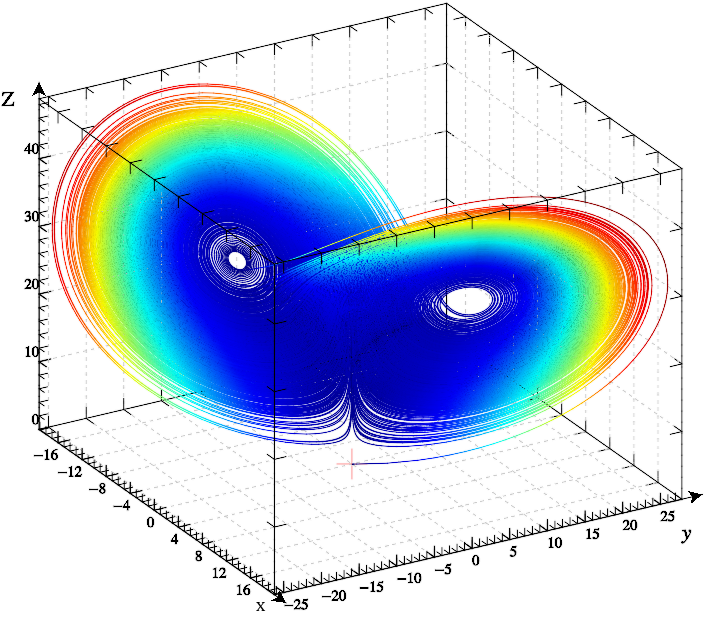
\includegraphics[width=0.42\textwidth]{p5/p/cha/lor/lor0-p_xyz_r=028_xl.png}
  \hfill
  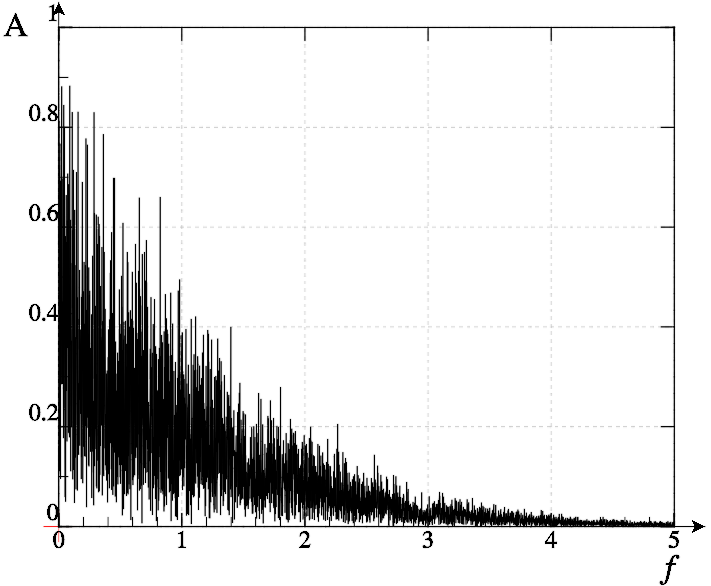
\includegraphics[width=0.42\textwidth]{p5/p/cha/lor/lor0_fft-p_f_r=028_xl.png}
  \hfill ~
\end{center}
\vspace{-2.5ex}
  \begin{center}
    ~ \hfill a \hfill\hfill b \hfill ~
  \end{center}
  \vspace{-2.5ex}
  \caption{Аттрактор (a) і спектр (b) системи Лоренца (\ref{atu:eq:lor}) в хаотичному режимі($r=28$)}
\label{atu:f:lor_attractor_phase_chaos28}
\end{figure}

Для синтезу критерію ідентифікації параметра $r$ системи
(\ref{atu:eq:lor}), розглянемо набір фізичних систем, для моделювання яких застосовується
система Лоренца. Історично першою такою системою є задача про теплову
конвекцію рідини в плоскому шарі.
Змінні і параметри системи Лоренца визначаються наступним чином: $x$ задає
швидкість обертання валів течії, $y$, $z$ --- відповідають розподілу
температури по горизонталі і вертикалі. $\sigma$ --- число Прандтля
(відношення коефіцієнтів кінематичної в'язкості і температуропровідності).
Параметр $b$ визначає відношення розмірів осередку, $r$ --- (ідентифікований
параметр) --- приведене число Релея, що визначає енергетичні параметри
конвективної течії.
З трьох змінних стану найпростішому спостереженню піддається змінна $x$.
З іншого боку, так як параметр $r$ визначає енергетичні співвідношення в
системі, то і критерій якості повинен являти собою квадратичну форму від $x$,
причому усереднену на інтервалі часу, значно більшому, ніж характерний час
обороту рідинного вала.

Виходячи з вищевикладеного, в першу чергу слід перевірити придатність критерію
виду $q_{x^2}$. Проте, перевіримо всі критерії даного виду, застосовні до
даної системи. На рис.~\ref{atu:f:lor_q} наведені досліджувані залежності
$q_{*}(r)$.

\begin{figure}[ht!]
  \centerline{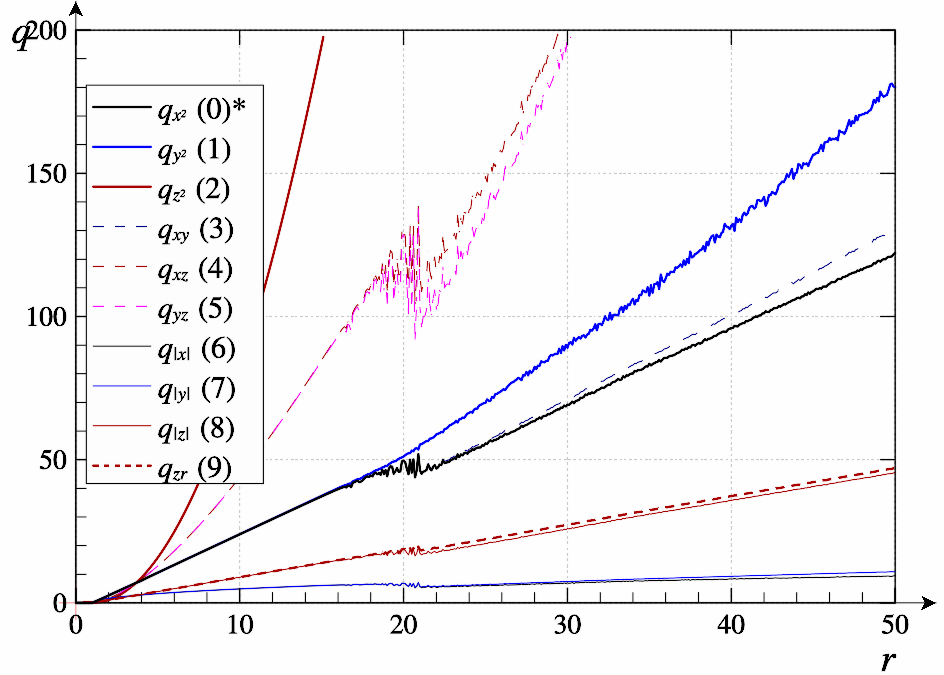
\includegraphics[width=0.55\textwidth]{p5/p/cha/lor/lor_q-p_q_r_xl.png} }
  \vspace{-2.0ex}
  \caption{Розглянуті критерії для системи Лоренца}
  \label{atu:f:lor_q}
\end{figure}

З аналізу графіків зроблено висновок, що практично всі розглянуті види
критеріїв повинні дозволяти побудувати працездатну систему ідентифікації. При
цьому, велика частина графіків, в тому числі і з самого початку запропонований
$q_{x^2}$, втрачають монотонність при переході від режиму загасаючих
коливань до хаотичного.
Спектри сигналів $x(t)$, $y(t)$ і $z(t)$ мають практично однакову
структуру. У подальших дослідженнях використовувалися критерії
$q_{x^2}$ та
$q_{y^2}$.
Також отримано залежності $\sigma_q(\tau_q)$ та  $\sigma_q(a_q)$,
що дозволяє коректно установити $a_q$.

Визначимо тестові завдання наступним чином:
\[
  p(t) \in [20, 60],
\]
%
\begin{equation}
  r_o(t) = p_o(t) = p_0 +  U_{p} \sign \sin( \omega_{p} t ),
  \label{atu:eq:lor_po_t_sign}
\end{equation}
%
%
\begin{equation}
  r_o(t) = p_o(t) = p_0 +  U_{p} \sin( \omega_{p} t ),
  \label{atu:eq:lor_po_t_sin}
\end{equation}
%
де:
$p_0 = 37$, $U_p=12$, $\omega_p=0.09$.

Розглянуто застосування для ідентифікації методу,
який використовує два УГПК і інтегратор для визначення динаміки одного агента,
який керує двома моделями
(``Fl2nlosdlcA.$q_{x^2}$''). Встановлено, що він
працездатний, але
не забезпечує потрібної швидкодії.
Для порівняння були обрані три групи мультімодельних метода ідентифікації:
ql3ruonAAF.$q_{x^2}$,
ql3ruonAAF.$q_{y^2}$ и
Fq3zlovnAAF.$q_{x^2}$.
На рис.~\ref{atu:f:lor_id_ql3ruonAAF.q_x2_sign} представлені результати
ідентифікації групою методів ql3ruonAAF.$q_{x^2}$.

\begin{figure}[ht!]
  \centerline{
    ~ \hfill
    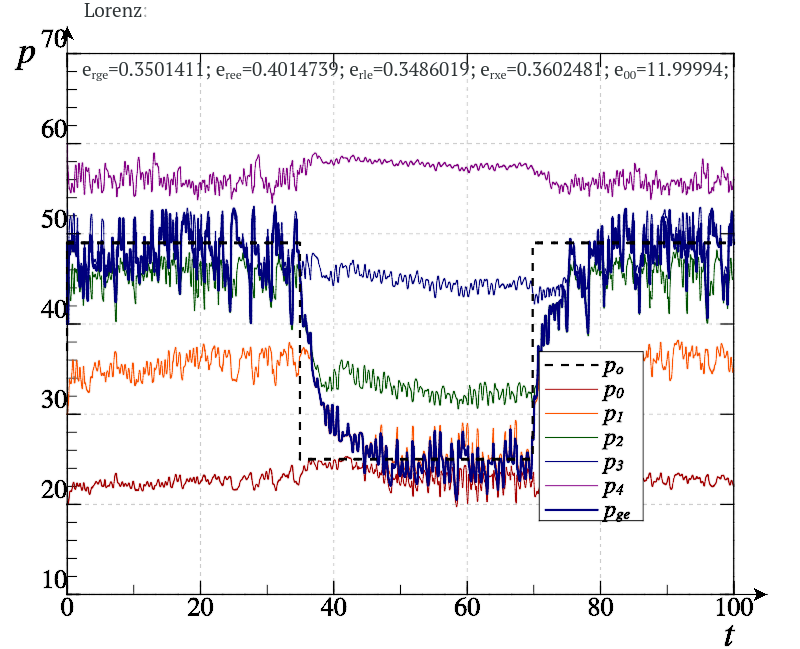
\includegraphics[width=0.45\textwidth]{p5/p/cha/lor/ql3ruonAAF/lor_ql3ruonAAF_qy2-p_t_pi_sign_xl.png}
    \hfill
    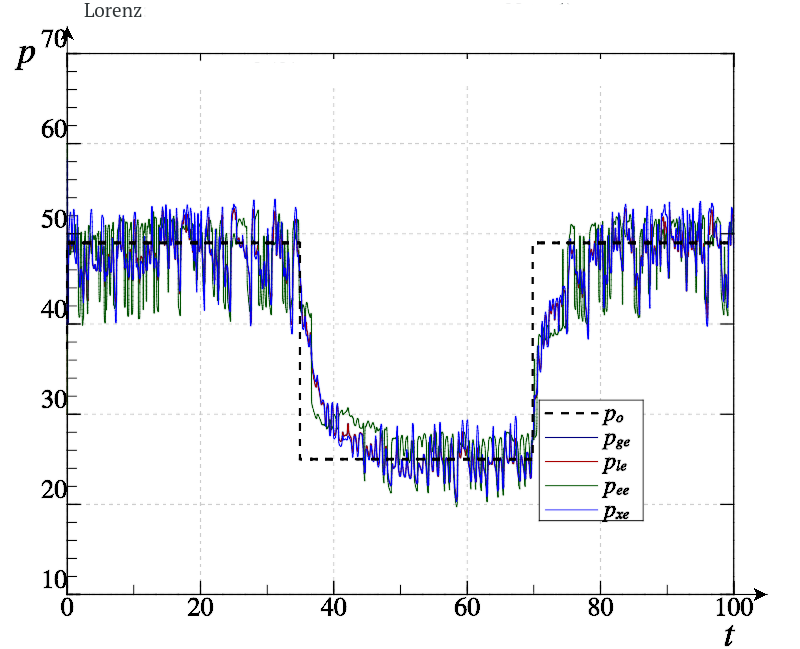
\includegraphics[width=0.45\textwidth]{p5/p/cha/lor/ql3ruonAAF/lor_ql3ruonAAF_qy2-p_t_pz_sign_xl.png}
    \hfill ~
  }
  \vspace{-1.5ex}
  \begin{center}
    ~ \hfill a \hfill\hfill b  \hfill ~
  \end{center}
  \vspace{-2.5ex}
  \caption{Процес ідентифікації параметра ``$r$'' системи Лоренца групою методів ql3ruonAAF.$q_{x^2}$ при умовах~(\ref{atu:eq:lor_po_t_sign}):
  динаміка агентів (a) і різні методи визначення $p_\mathrm{id}$ (b)}
  \label{atu:f:lor_id_ql3ruonAAF.q_x2_sign}
\end{figure}

Найгірші результати демонструє $p_{ge}$. Також, абсолютно очікувано, кращі
результати продемонстрував підхід $ p_{be}$. Також, при штучних обмеження
$v_f = 0$ і $q_\gamma = 0.1$ були отримані величини, що характеризують
якість ідентифікації для нерухомих агентів:
$\overline{e}_{bc} = 9.85$ і
$\overline{e}_{be} = 7.09$, що свідчить про виправданість як переміщення
агентів, так і використання величин $p_e$ для визначення $p_\mathrm{id}$.
Аналогічні результати, але з меншою похибкою ідентифікації були отримані за
умови плавної зміни значення параметра об'єкта~(\ref{atu:eq:lor_po_t_sin}).

Процес ідентифікації групою методів Fq3zlovnAAF за умовами~(\ref{atu:eq:lor_po_t_sign}) представлено
на рис.~\ref{atu:f:lor_id_Fq3zlovnAAF.q_x2_sign}. В першу чергу слід
відзначити велику рухливість агентів, аж до штучного обмеження рухливості
більшості моделей. З одного боку, це дещо зменшує швидкодію системи при
різких змінах параметра, з іншого --- забезпечує достатнє зміщення ``далеких''
агентів, що, в якійсь мірі, компенсує можливі похибки в налаштовуванні системи.

\begin{figure}[ht!]
  \centerline{
    ~ \hfill
    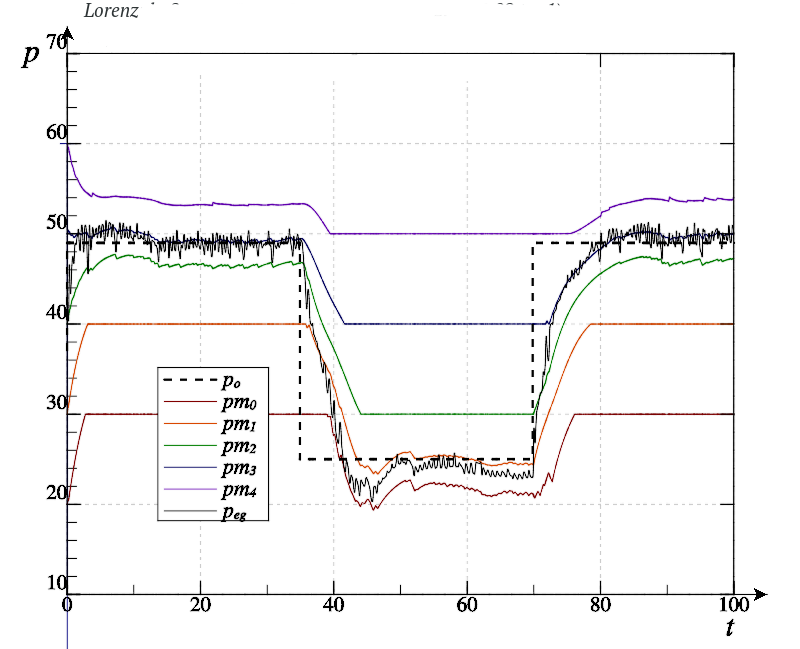
\includegraphics[width=0.45\textwidth]{p5/p/cha/lor/Fq3zlovnAAF/lor_Fq3zlovnAAF_qx2-pl_n_sign_xl.png}
    \hfill
    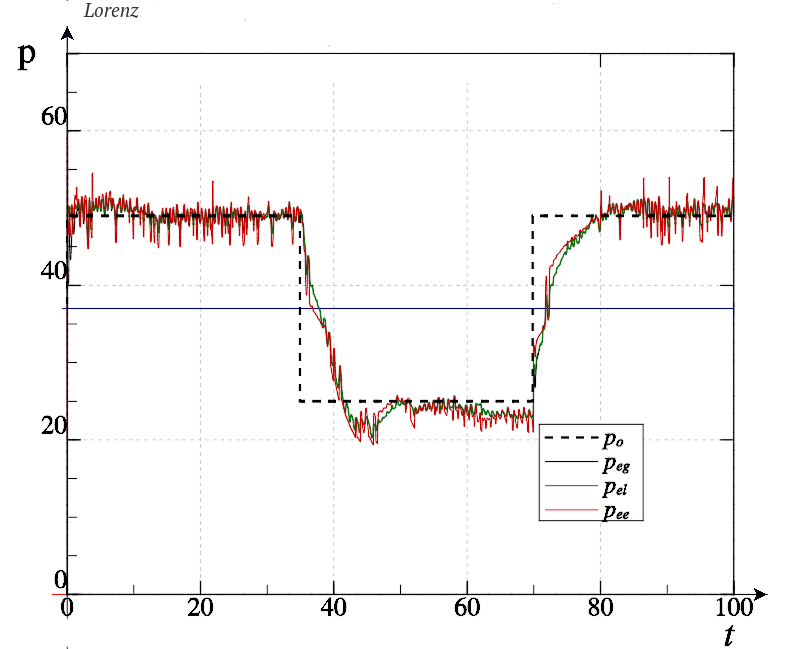
\includegraphics[width=0.45\textwidth]{p5/p/cha/lor/Fq3zlovnAAF/lor_Fq3zlovnAAF_qx2-p_p_sign_xl.png}
    \hfill ~
  }
  \vspace{-1.5ex}
  \begin{center}
    ~ \hfill a \hfill\hfill b  \hfill ~
  \end{center}
  \vspace{-2.5ex}
  \caption{Процес ідентифікації параметра ``$r$'' системи Лоренца групою методів Fq3zlovnAAF.$q_{x^2}$ при умовах~(\ref{atu:eq:lor_po_t_sign}):
  динаміка агентів (a) і різні методи визначення $p_\mathrm{id}$ (b)}
  \label{atu:f:lor_id_Fq3zlovnAAF.q_x2_sign}
\end{figure}


Розглянуто вплив параметрів системи ідентифікації на процес ідентифікації. Для
цього кожен з істотних параметрів змінювався та досліджувались
залежності $\overline {e}_{r}$ для кожного з розглянутих методів.
Як приклад,
на рис.~\ref{atu:f:lor_a_q_ql3ruonAAF.q_x2} представлені залежності
усереднених помилок ідентифікації системи Лоренца від $a_q$ при використанні
групи методів ql3ruonAAF.
Форма кривих з явним екстремумом обумовлена впливами протидіючих
факторів. При великих значеннях $a_q$, є занадто сильний вплив хаотичної
динаміки, та намає можливості проводити успішну ідентифікацію. З іншого боку, при
занадто малих значеннях $a_q$, час оцінювання критерію настільки зростає, що
система ідентифікації не встигає відстежувати зміну параметра.

\begin{figure}[ht!]
  \centerline{
    ~ \hfill
    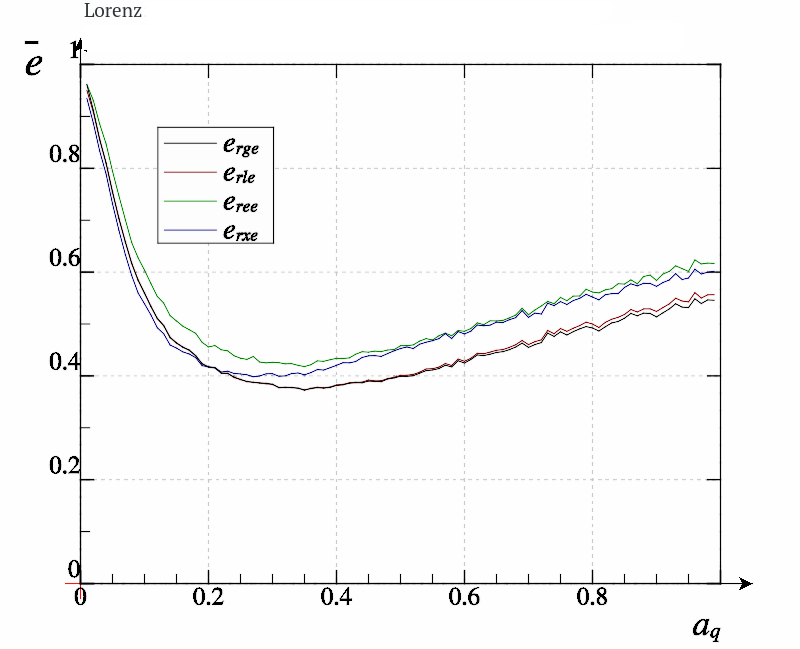
\includegraphics[width=0.45\textwidth]{p5/p/cha/lor/ql3ruonAAF/lor_ql3ruonAAF_qx2-p_a_q_e_sign_xl.png}
    \hfill
    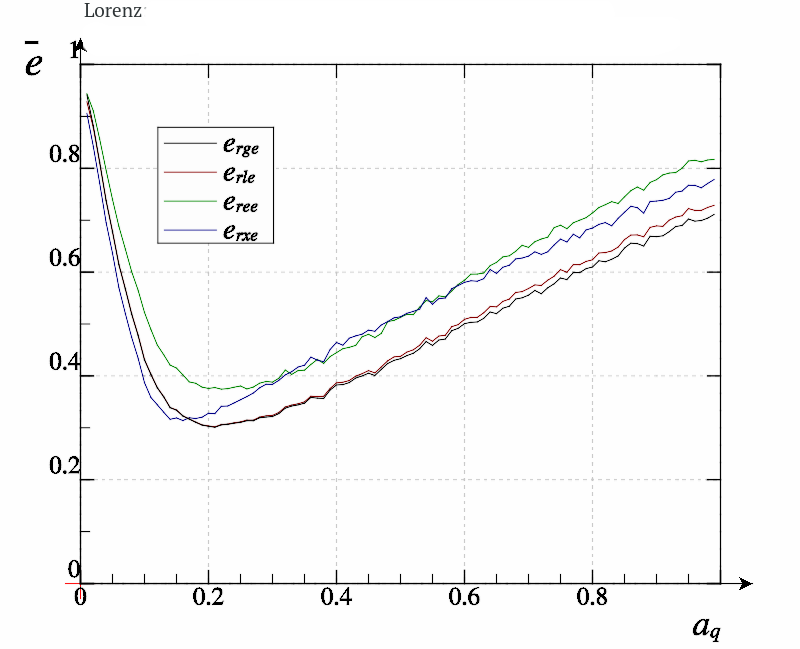
\includegraphics[width=0.45\textwidth]{p5/p/cha/lor/ql3ruonAAF/lor_ql3ruonAAF_qx2-p_a_q_e_sin_xl.png}
    \hfill ~
  }
  \vspace{-1.5ex}
  \begin{center}
    ~ \hfill a \hfill\hfill b  \hfill ~
  \end{center}
  \vspace{-2.5ex}
  \caption{Залежності $\overline{e}_{r}(a_q)$ при ідентифікації системи Лоренца групою методів ql3ruonAAF.$q_{x^2}$
   при умовах ~(\ref{atu:eq:lor_po_t_sign}) (a) та (\ref{atu:eq:lor_po_t_sin}) (b)}
  \label{atu:f:lor_a_q_ql3ruonAAF.q_x2}
\end{figure}

Також розглянуто вплив параметрів $q_\gamma$, $v_f$, $k_e$, $k_n$, $k_c$.
Визначено, що адаптивні властивості мультиагентних ансамблевих пошукових методів дозволяють
змінювати параметри системи ідентифікації в широких межах,
що спрощує настроювання ті забезпечує робастність метода.
Вид функції якості має вплив на результати, але не суттєвий.
Також встановлено, що як занадто мала, так і занадто велика кількість агентів
приводить до росту похибки ідентифікації.

Для оцінки можливості одночасної ідентифікації декількох параметрів
розглянуто графіки залежностей критеріїв, за умови зміни двох параметрів
попарно: ($r$, $\sigma$) і ($r$, $b$).
На рис.~\ref{atu:f:lor_qz2_r_b}
приведена залежність
$q_{z^2}(r,b)$.
Близька до квадратичної залежність від параметра $r$ не представляє особливих
проблем. Корисним є той факт, що для даного критерію залежність від параметра $b$
досить мала. Отже, при двопараметричной ідентифікації даний критерій має
сенс використовувати для (оціночної) ідентифікації параметра $r$, і
сукупність даного критерію разом з, наприклад, $q_{x^2}$ дозволить
ідентифікувати обидва параметри без використання надмірної кількості моделей.

\begin{figure}[ht!]
  \centerline{  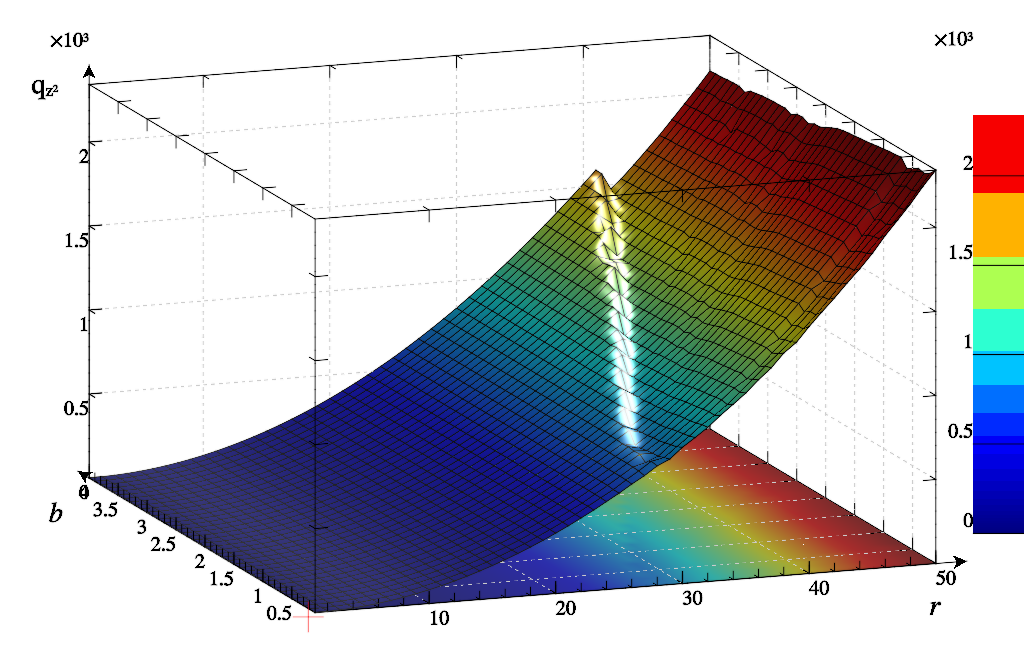
\includegraphics[width=0.50\textwidth]{p5/p/cha/lor/q2d/lor_qz2_r_b.png}  }
  \caption{Залежність $q_{z^2}(r,b)$ для системи Лоренца}
  \label{atu:f:lor_qz2_r_b}
\end{figure}


Таким чином,
для синтезу працездатної системи ідентифікації параметра ``$r$'' системи
Лоренца можуть застосовуватися практично всі розглянуті критерії. При цьому,
більший діапазон використання --- у критерію  $q_{x^2}$.
Система мультиагентної ідентифікації може бути реалізована як з агентами, які
здійснюють пошук як з використанням критерію, так і з використанням функції
якості. При цьому, похибка ідентифікації визначається в основному не конкретним
методом, а динамічними властивостями самого ідентифікованого об'єкта і
часом усереднення критерію.


Розглянуто систему, що позначається як ``Sprott~A''. Відмінною
особливістю цієї системи є відсутність положень рівноваги, що унеможливлює
застосування багатьох відомих методів аналізу, заснованих на будь-якому
розкладі в околі точок рівноваги.
Додамо до системи параметр $c_{x_y}$:
% %
% \begin{equation}
%   \begin{cases}
%     \dot{x} =  y, \\
%     \dot{y} = -x + yz, \\
%     \dot{z} =  1 - y^2.
%   \end{cases}
%   \label{atu:eq:spr_a_orig}
% \end{equation}
%
%
\begin{equation}
  \begin{cases}
    \dot{x} =  c_{x_y} y, \\
    \dot{y} = -x + yz, \\
    \dot{z} =  1 - y^2.
  \end{cases}
  \label{atu:eq:spr_a}
\end{equation}

У такому вигляді система, при зміні $c_{x_y}$ в досить широкому діапазоні
демонструє як складно-періодичну, так і переважно, хаотичну поведінку
(рис.~\ref{atu:f:spr_a_p_0610}).

\begin{figure}[htb!]
\centerline{
  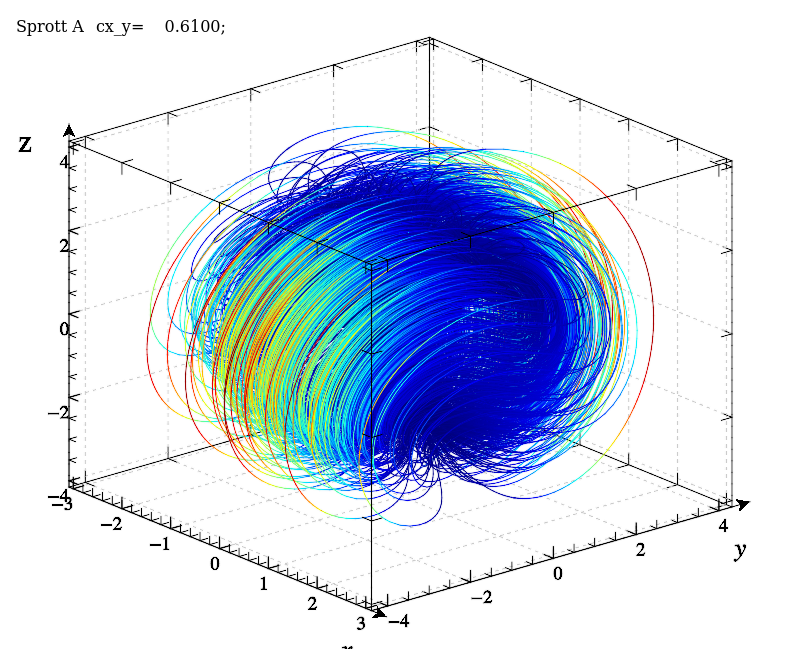
\includegraphics[width=0.42\textwidth]{p5/p/cha/spr_a/sprott_a-p_xyz_cx_y=0x610.png}
  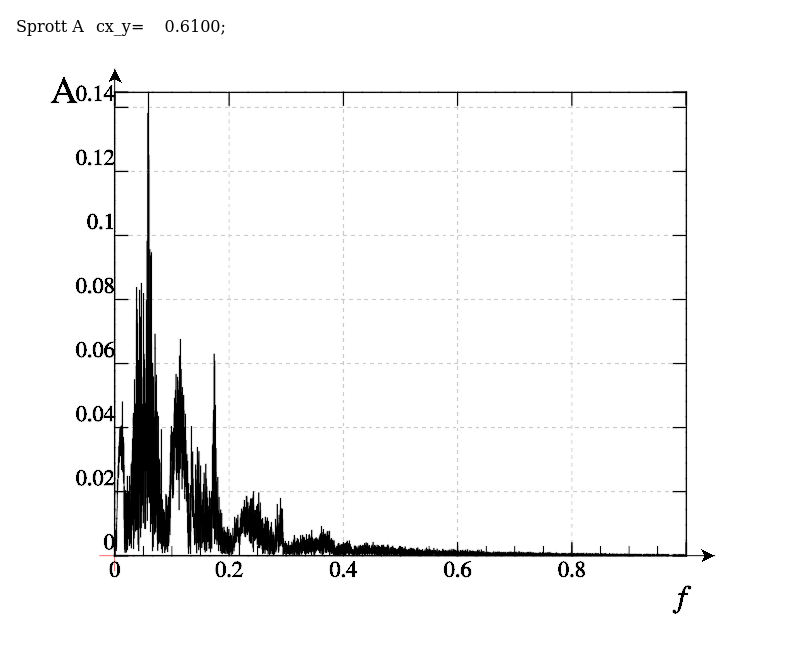
\includegraphics[width=0.42\textwidth]{p5/p/cha/spr_a/sprott_a_f-p_f_cx_y=0x610.png}
}
  \vspace{-1.5ex}
  \begin{center}
    ~ \hfill a \hfill\hfill b \hfill ~
  \end{center}
  \vspace{-2.5ex}
  \caption{Аттрактор (a) та спектр (b) системи (\ref{atu:eq:spr_a}) при $c_{x_y} =0.610$}
\label{atu:f:spr_a_p_0610}
\end{figure}

Розглянемо залежності $q(c_{x_y})$ (рис.~\ref{atu:f:spr_a_q})
для системи (\ref{atu:eq:spr_a}). Аналіз цих залежностей дає
відповідь про можливий вид критерію --- $q_{x^2}$.

\begin{figure}[htb!]
\centerline{
  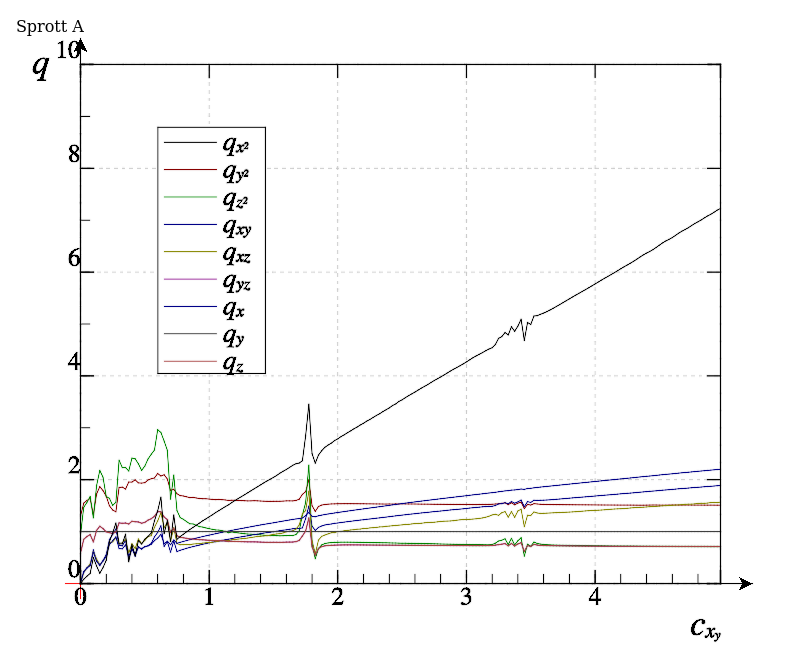
\includegraphics[width=0.45\textwidth]{p5/p/cha/spr_a/sprott_a_q-p_c_x_y.png}
}
\caption{Залежності $q(c_{x_y})$ для системи (\ref{atu:eq:spr_a}) }
\label{atu:f:spr_a_q}
\end{figure}

В околі точки $c_{x_y} = 1.775$ атрактор також різко змінює свою
структуру. Так як це досить вузький окіл, то можна припустити, що
мультиагентна система ідентифікації не опиниться непрацездатною в цій області,
просто виросте похибка ідентифікації.

Визначимо тестове завдання наступним чином:
\[
  c_{x_y}(t) \equiv p_o(t) \in (0, 5],
\]
%
\begin{equation}
  p_o(t) = p_0 +  U_{p} \sign \sin( \omega_{p} t ),
  \label{atu:eq:spr_a_po_t_sign}
\end{equation}
%
%
\begin{equation}
  p_o(t) = p_0 +  U_{p} \sin( \omega_{p} t ),
  \label{atu:eq:spr_a_po_t_sin}
\end{equation}
%
де:
$p_0 = 2.8$, $U_p=1.9$, $\omega_p=0.04$.

На рис.~\ref{atu:f:spr_a_id_ql3rlWvnAAW.q_x2_sign}
представлені результати моделювання процесу ідентифікації групою методів ql3rlWvnAAW.$q_{x^2}$.
Залежність $p_{gc} (t)$, в даному випадку демонструє високий
рівень коливань, і отже, гірші результати пошуку. При цьому, інші підходи до
визначення $p_\mathrm{id}$ демонструють схожі між собою результати.

\begin{figure}[ht!]
  \centerline{
    ~ \hfill
    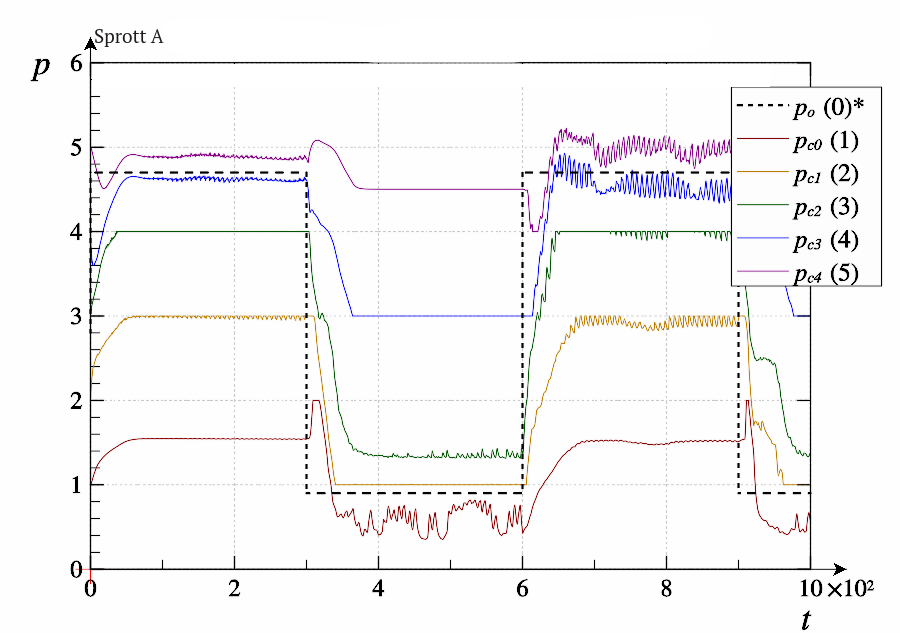
\includegraphics[width=0.49\textwidth]{p5/p/cha/spr_a/ql3rlWvnAAW_x2/sprott_a_id-p_t_pi_ql3rlWvnAAW_sign_xl.png}
    \hfill
    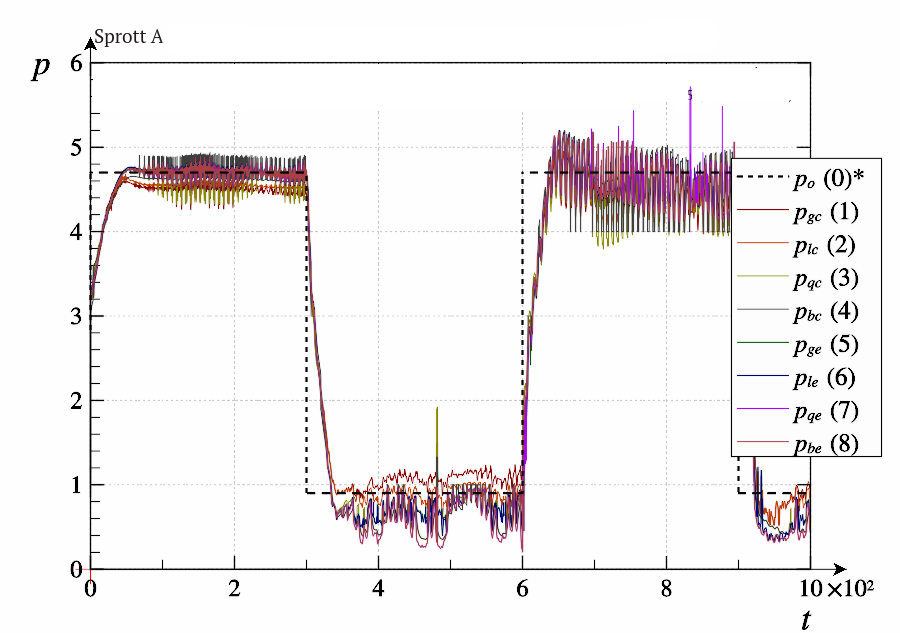
\includegraphics[width=0.49\textwidth]{p5/p/cha/spr_a/ql3rlWvnAAW_x2/sprott_a_id-p_t_p_ql3rlWvnAAW_sign_xl.png}
    \hfill ~
  }
  \vspace{-1.5ex}
  \begin{center}
    ~ \hfill a \hfill\hfill b \hfill ~
  \end{center}
  \vspace{-2.5ex}
  \caption{Процес ідентифікації параметра ``$c_{x_y}$'' системи Sprott A групою методів ql3rlWvnAAW.$q_{x^2}$ при умовах~(\ref{atu:eq:spr_a_po_t_sign})
  динаміка агентів (a) і різні методи визначення $p_\mathrm{id}$ (b)}
  \label{atu:f:spr_a_id_ql3rlWvnAAW.q_x2_sign}
\end{figure}

На рис.~\ref{atu:f:spr_a_id_Fq3rlFvnAAF.q_x2_sign}
представлені результати ідентифікації групою методів
Fq3rlFvnAAF.$q_{x^2}$.


\begin{figure}[ht!]
  \centerline{
    ~ \hfill
    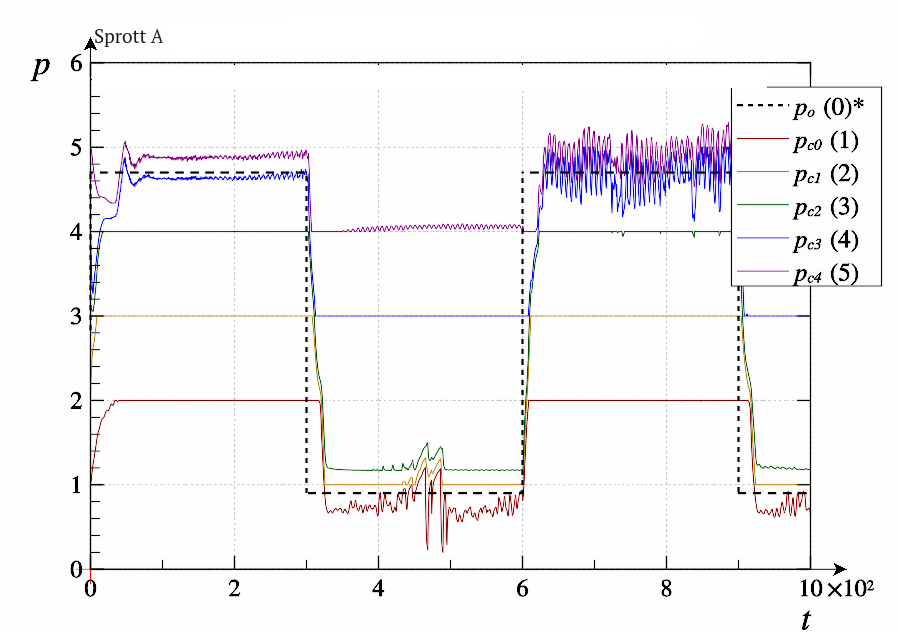
\includegraphics[width=0.49\textwidth]{p5/p/cha/spr_a/Fq3rlFvnAAF_x2/sprott_a_id-p_t_pi_Fq3rlFvnAAF_sign_xl.png}
    \hfill
    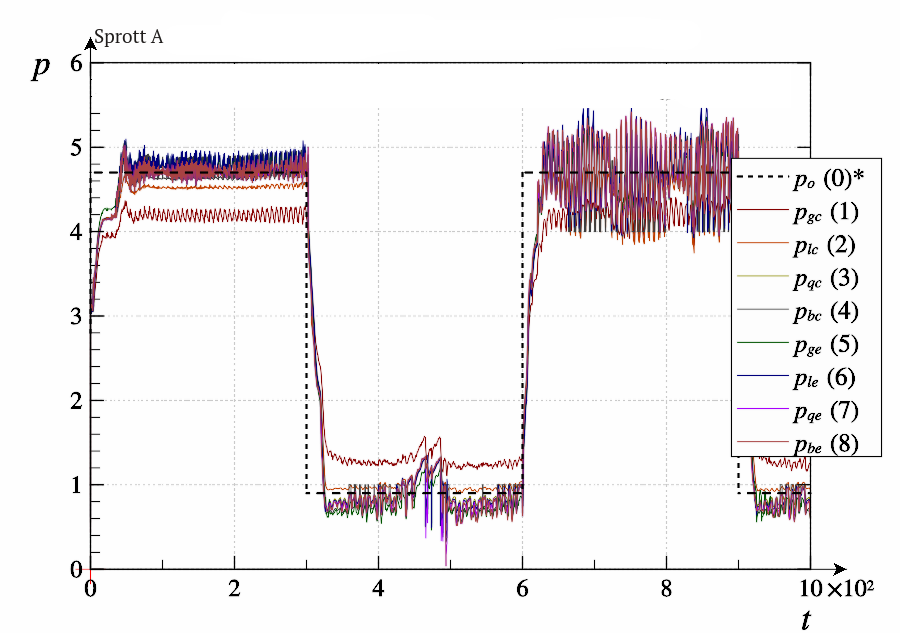
\includegraphics[width=0.49\textwidth]{p5/p/cha/spr_a/Fq3rlFvnAAF_x2/sprott_a_id-p_t_p_Fq3rlFvnAAF_sign_xl.png}
    \hfill ~
  }
  \vspace{-1.5ex}
  \begin{center}
    ~ \hfill a \hfill\hfill b \hfill ~
  \end{center}
  \vspace{-2.5ex}
  \caption{Процес ідентифікації параметра ``$c_{x_y}$'' системи Sprott A групою методів Fq3rlFvnAAF.$q_{x^2}$ при умовах~(\ref{atu:eq:spr_a_po_t_sign})
  динаміка агентів (a) і різні методи визначення $p_\mathrm{id}$ (b)}
  \label{atu:f:spr_a_id_Fq3rlFvnAAF.q_x2_sign}
\end{figure}

При наявності різниці у динаміці агентів, загальна похибка ідентифікації
має той же порядок.

Також розглянуто вплив параметрів $a_q$, $q_\gamma$, $v_f$, $k_e$, $k_n$, $k_c$
на якість ідентифікації. Як і для системи Лоренца, методи
продемонстрували достатню робасність, але для цієї системи
вплив динаміки агентів значно менший.

Однією з відомих хаотичних систем, легко реалізованих як аналітично,
(\ref{atu:eq:chua}), так і схемотехнічно, є нелінійна система Чуа:
%
\begin{equation}
\begin{cases}
  C_1 \dot{V_1}  = \frac{1}{R} ( V_2 - V_1 ) - g(V_1), \\
  C_2 \dot{V_2}  = \frac{1}{R} ( V_1 - V_2 ) + I_L, \\
  \dot{I_L}      = - \frac{1}{L} V_2 .
\end{cases}
\label{atu:eq:chua}
\end{equation}

Єдиним нелінійним елементом в цій системі є ``діод Чуа'' з характеристикою
$g(V)$~(\ref{atu:eq:diodchua}).
%
%
\begin{equation}
g(V) =
\begin{cases}
  m_1 V = ( m_0 + m_2 ) V , & |V| <   U_0, \\
  m_0 V ,                   & |V| \ge U_0.
\end{cases}
\label{atu:eq:diodchua}
\end{equation}

Введемо параметр \(m_2 = m_1 - m_0 \), який визначає в цілому нелінійність
системи. У даній роботі як параметр, що підлягає ідентифікації, розглядається саме~$m_2$.
Класично параметри системи Чуа задаються наступним чином:
$C_1 = 1/9$, $C_2 = 1$, $L= 1/7$, $R = 1/0.7$, $m_0=-0.5$, $ m_2 \in [ -0.15; -0.7 ] $.

Введемо позначення:
\[
  a_{11} = \frac{1}{R C_1}; \;
  a_{13} = \frac{1}{C_1}; \;
  a_{21} = \frac{1}{R C_2}; \;
  a_{23} = \frac{1}{C_2}; \;
  a_{31} = -\frac{1}{L}; \;
  a_g = - \frac{m_0}{C_1}; \;
  \mu = - \frac{m_2}{C_1}.
\]
%
%\noindent
Тоді
%
\begin{equation}
\begin{cases}
  \dot{V}_1  = -a_{11} V_1 + a_{11}  V_2  + g_1(V_1) , \\
  \dot{V}_2  = +a_{21} V_1 - a_{21}  V_2  + a_{23} I_L    , \\
  \dot{I}_L  =  a_{31} V_2.
\end{cases}
\label{atu:eq:chua2}
\end{equation}
%
%
\begin{equation}
g_1(V) =
\begin{cases}
  ( a_g + \mu ) V , & |V| <   U_0, \\
  a_g V           , & |V| \ge U_0.
\end{cases}
\label{atu:eq:diodchua2}
\end{equation}

\noindent
$a_{11} = 6.5$,
$a_{21} = 0.7$,
$a_{23} = -7$,
$a_g = 4.5$,
$\mu \in [ 1.29 ; 5.6 ]$.
Відповідно, в цих позначеннях ідентифікований параметр є~$\mu$.
Він задає динаміку системи.
% (рис.~\ref{atu:eq:chua2}).
%
% \begin{figure}[htb!]
% \centerline{
%   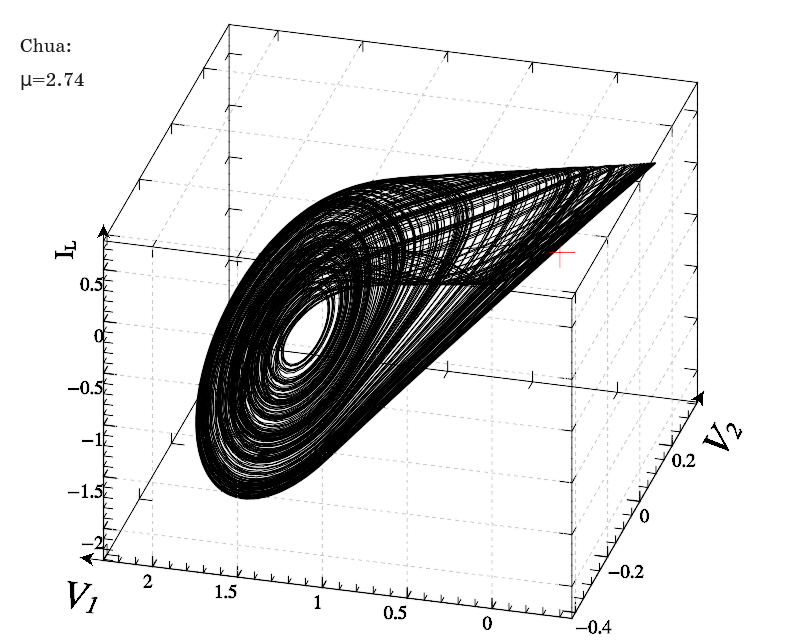
\includegraphics[width=0.42\textwidth]{p5/p/cha/chua/chua_1-p_xyz_mu=2x74.png}
%   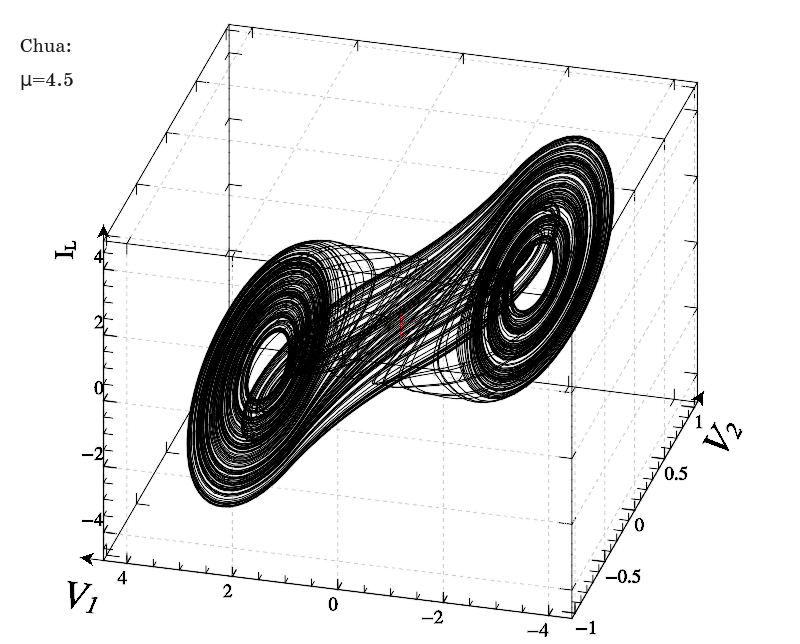
\includegraphics[width=0.42\textwidth]{p5/p/cha/chua/chua_1-p_xyz_mu=4x50.png}
% }
% \caption{Аттрактор системи Чуа (\ref{atu:eq:chua2}) при різних значеннях $\mu$}
% \label{atu:f:chua_phase}
% \end{figure}

Для визначення виду критерію розглянемо залежності $ q_{*}(\mu)$ отримані
шляхом моделювання системи Чуа (рис.~\ref{atu:f:chua_q}):

\begin{figure}[htb!]
\centerline{
  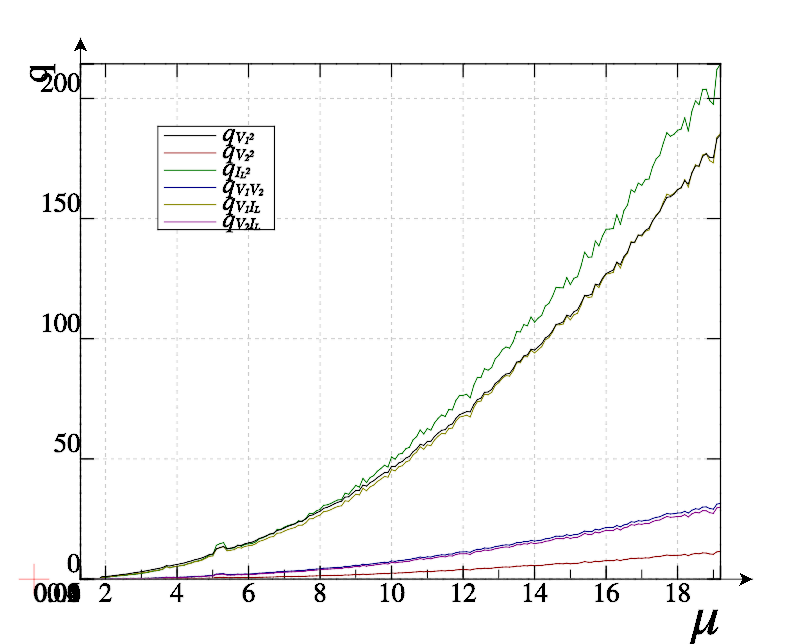
\includegraphics[width=0.45\textwidth]{p5/p/cha/chua/chua_q-p_mu2.png}
  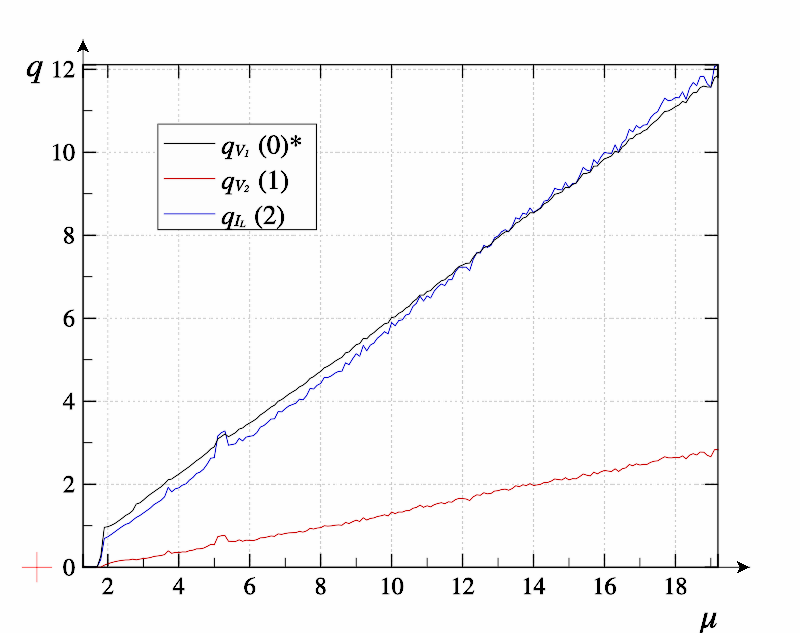
\includegraphics[width=0.45\textwidth]{p5/p/cha/chua/chua_q-p_mu1.png}
}
  \caption{Залежності $q_{*}(\mu)$ для системи Чуа (\ref{atu:eq:chua2})}
\label{atu:f:chua_q}
\end{figure}

З аналізу графіків зроблено висновок, що величина $q_{V_1}(\mu)$
є найкращим кандидатом в критерії, з огляду на близьку до лінійної залежності в робочому діапазоні.
%
Для ідентифікації було використано різні методи, у цілому найкращі результати було
отримано для групи методів ``ql3rlWvnAAW''.
% Для
% дослідження динамічних властивостей системи ідентифікації параметр $\mu_o$
% для об'єкта задавався двома способами:
% %
% \begin{equation}
%  \mu_o(t) = p_0 + U_p \sign \sin( \omega_p t )
%   \label{atu:eq:chua_mu_sign}
% \end{equation}
% %
% \begin{equation}
%  \mu_o(t) = p_0 + U_p \sin( \omega_p t ).
%   \label{atu:eq:chua_mu_sin}
% \end{equation}

Динаміка процесів ідентифікації системи Чуа представлена на рис.~\ref{atu:f:chua_id}.

\begin{figure}[htb!]
\centerline{
    ~ \hfill
    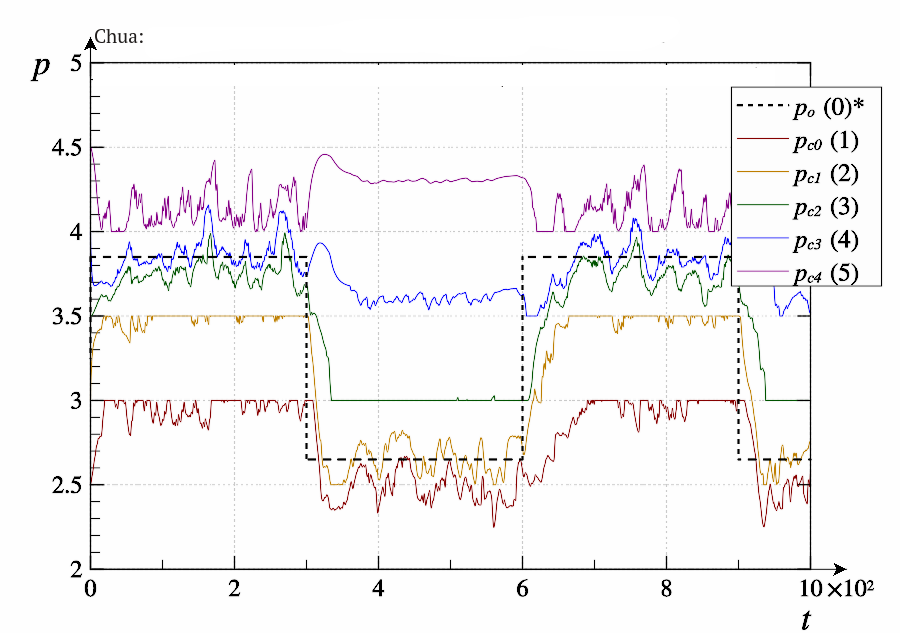
\includegraphics[width=0.49\textwidth]{p5/p/cha/chua/ql3rlWvnAAW/chua_id-p_t_pi_ql3rlWvnAAW_sign_xl.png}
    \hfill
    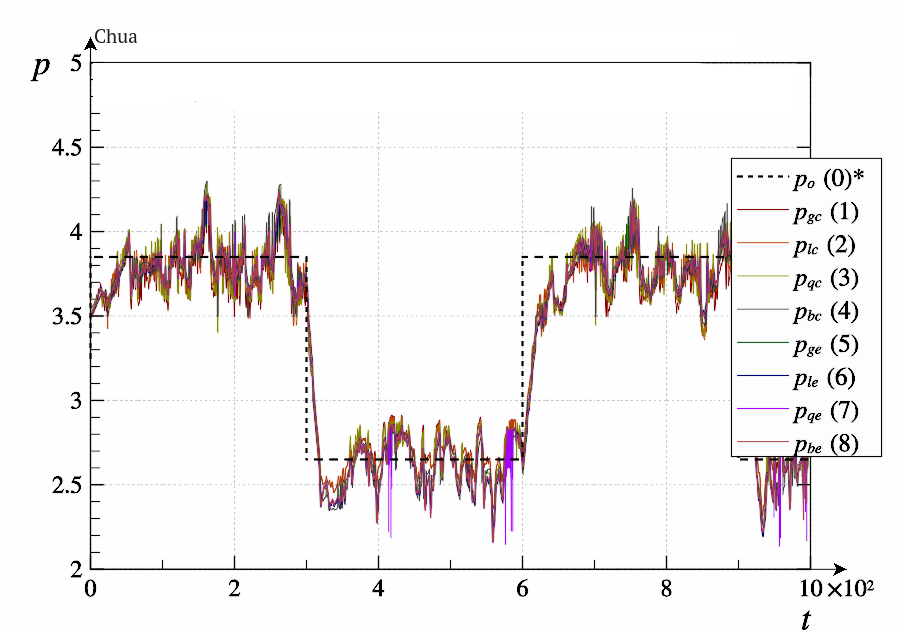
\includegraphics[width=0.49\textwidth]{p5/p/cha/chua/ql3rlWvnAAW/chua_id-p_t_p_ql3rlWvnAAW_sign_xl.png}
    \hfill ~
}
  \vspace{-1.5ex}
  \begin{center}
    ~ \hfill a \hfill\hfill b \hfill ~
  \end{center}
  \vspace{-2.5ex}
\caption{Процес ідентифікації параметра $\mu$ системы (\ref{atu:eq:chua2})
  динаміка агентів (a) і різні методи визначення $p_\mathrm{id}$ (b)
  %при умовах (\ref{atu:eq:chua_mu_sign}) та (\ref{atu:eq:chua_mu_sin})
}
\label{atu:f:chua_id}
\end{figure}

Також розглянуто вплив параметрів $a_q$, $q_\gamma$, $v_f$, $k_e$, $k_n$, $k_c$
на якість ідентифікації. Методи
продемонстрували працездатність та робастність.


Існують динамічні системи, що не демонструють хаотичну поведінку,
але проявляють подібні властивості з точки зору ідентифікації. А саме,
безпосереднє порівняння виходів системи і моделі не дозволяє зробити ніяких
висновків про співвідношення між параметрами моделі і об'єкта. Одним із
прикладів таких систем є динамічна система (\ref{atu:eq:dryfric_sys}), що
моделює поведінку тіла заданої маси під дією зовнішньої сили, і сили
сухого тертя: %~\cite{atu_asau11}:
%
\begin{equation}
  m \ddot{x} + f_{df}( x, \dot{x}, \ldots)  = u(t).
\label{atu:eq:dryfric_sys}
\end{equation}
%
%\noindent
де
$m$ --- маса тіла,
$u(t)$ --- сила, що приводить до руху,
$f_{df}( x, \dot{x}, \ldots)$ --- сила сухого тертя.

Важливою особливістю при моделюванні сили сухого тертя є той факт, що це силу
неможливо коректно описати аналітично. Основним параметром, в найпростішому
випадку, що визначає силу сухого тертя, є $f_{dm}$ --- максимальна значення її
модуля. Визначення величини  $f_{dm}$ і будемо вважати метою задачі ідентифікації
системи з сухим тертям.

На рис.~\ref{atu:f:fric_outs}
представлено порівняльний приклад динаміки трьох моделей,
при однаковому вхідному сигналі і різних значеннях $f_{dm}$.

Для забезпечення можливості застосування методів ідентифікації, необхідне
існування критерію $q (x (t))$, що задовольняє наступним вимогам: чутливість
до динаміки моделі і об'єкта, властивість астатизму, достатня стійкість до
шумів вимірювання, фізична реалізація.

У даній роботі зроблено припущення, що рівень шумів дозволяє створити фільтр, який
дозволяє відсівати шуми за (як максимум) характерний час реакції системи. Після
фільтра діє реальна ланка, що диференціює. Відповідний вид критерію позначимо як
$q_{dx}$ (рис.~\ref{atu:f:fric_q}).


\begin{figure}[htb!]
  {~} \hfill
  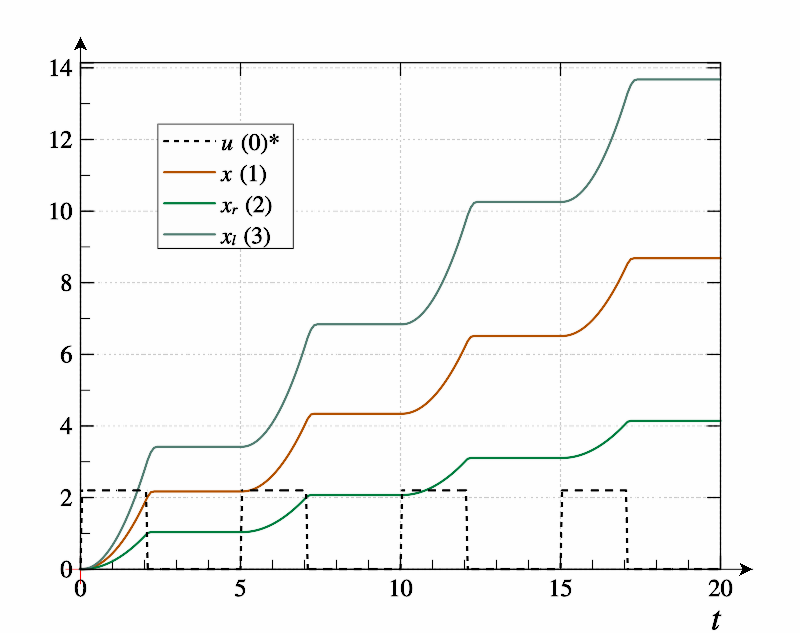
\includegraphics[width=0.40\textwidth]{p5/p/cha/fric/fric_outs1.png}
  \hfill
  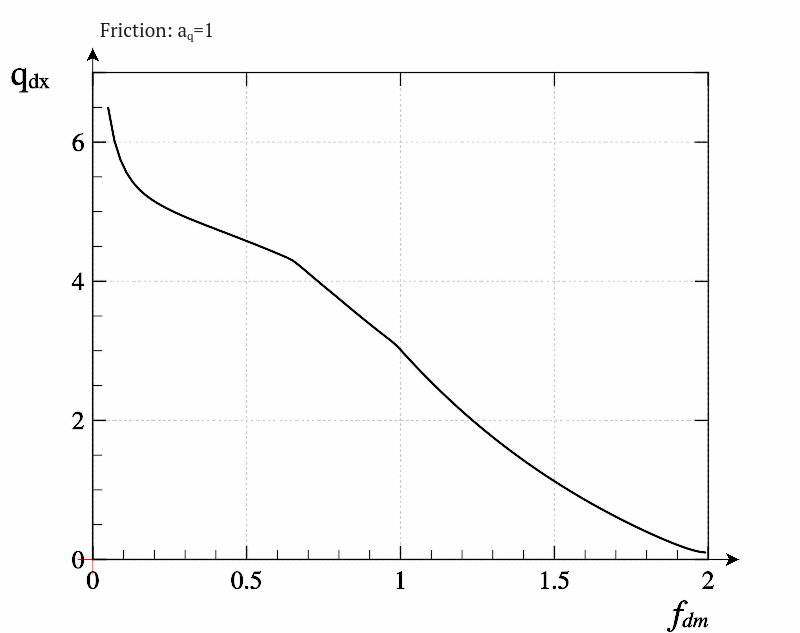
\includegraphics[width=0.40\textwidth]{p5/p/cha/fric/fric_q-p_f_dm_q.png}
  \hfill {~}
  \\
  \parbox[t]{0.48\textwidth} {
    \caption{Динаміка трьох моделей виду (\ref{atu:eq:dryfric_sys})}
    \label{atu:f:fric_outs}
  } \hfill
  \parbox[t]{0.48\textwidth} {
    \caption{Залежність $q_{dx}(f_{dm})$ для системи (\ref{atu:eq:dryfric_sys}) }
    \label{atu:f:fric_q}
  }
\end{figure}

Динаміка процесів ідентифікації для системи (\ref{atu:eq:dryfric_sys})
представлена на рис.~\ref{atu:f:fric_id}.
За винятком області, в якій критерій перестає працювати,
спостерігається досить низький рівень помилок ідентифікації. В першу чергу це
обумовлено тим, що дана система не є хаотичною, і проявляє тільки деякі подібні
властивості. І як наслідок, критерій, заснований на фізичних властивостях
системи дозволяє створити систему ідентифікації з низьким рівнем помилок.

\begin{figure}[htb!]
\centerline{
  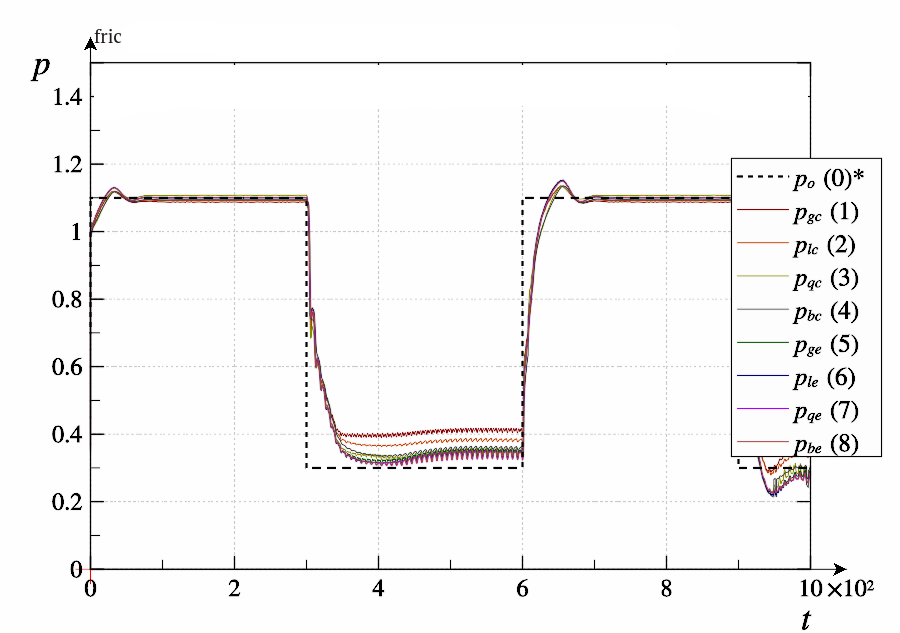
\includegraphics[width=0.49\textwidth]{p5/p/cha/fric/ql3rlWvnAAW/fric_id-p_t_p_ql3rlWvnAAW_sign_xl.png}
  \hfill
  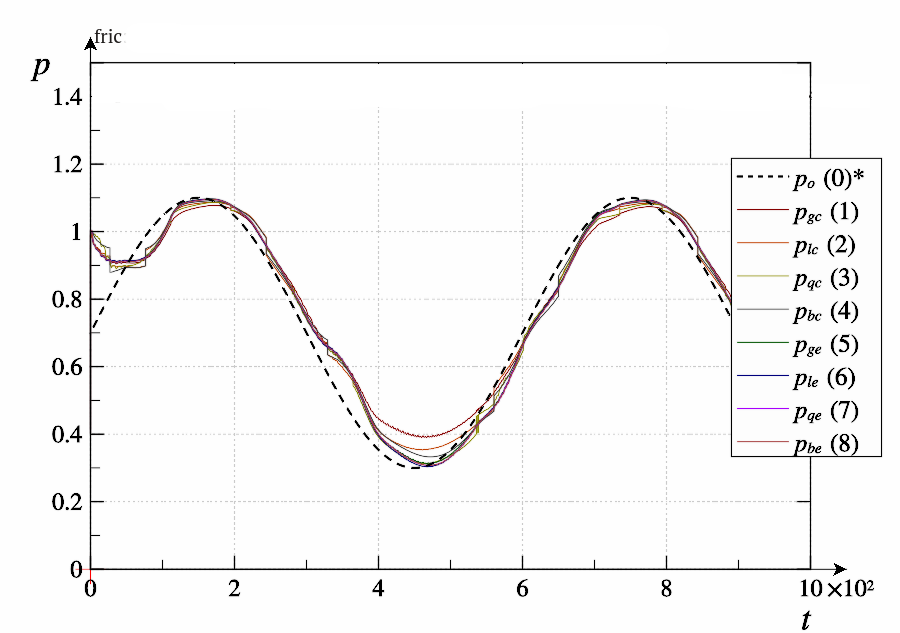
\includegraphics[width=0.49\textwidth]{p5/p/cha/fric/ql3rlWvnAAW/fric_id-p_t_p_ql3rlWvnAAW_sin_xl.png}
}
  \vspace{-1.5ex}
  \begin{center}
    ~ \hfill a \hfill\hfill b \hfill ~
  \end{center}
  \vspace{-2.5ex}
\caption{
  Процес ідентифікації параметра $f_{dm}$ системи (\ref{atu:eq:dryfric_sys}) групою методів ``ql3rlWvnAAW''
  при умовах (\ref{atu:eq:po_t_sign})~(a) і  (\ref{atu:eq:po_t_sin})~(b)
}
\label{atu:f:fric_id}
\end{figure}

Для даної системи енергетичні критерії, аналогічні застосованим в попередніх
випадках, виявилися непридатними. Критерій, хоч і заснований на вимірюванні
похідною (після фільтрації), виявився працездатним. В першу чергу це пов'язано
з тим, що в основі були покладені фізичні принципи.


Також у розділі досліджуються процеси ідентифікації системи Дуффінга, Ван-дер-Поля,
вібраційної системи із гістерезисом у силі, що повертає.


\textbf{У п'ятому розділі}
розглянуте практичне застосування
нових методів ідентифікації для генератора Колпітца
з використанням реального фізичного об'єкту.
Параметром, що підлягає ідентифікації, було обрано $R_c$.
На рис.~\ref{atu:f:colp_schem_real} представлена електрична схема реалізації
генератора Колпітца, яка була використана у даній роботі.

\begin{figure}[htb!]
\centerline{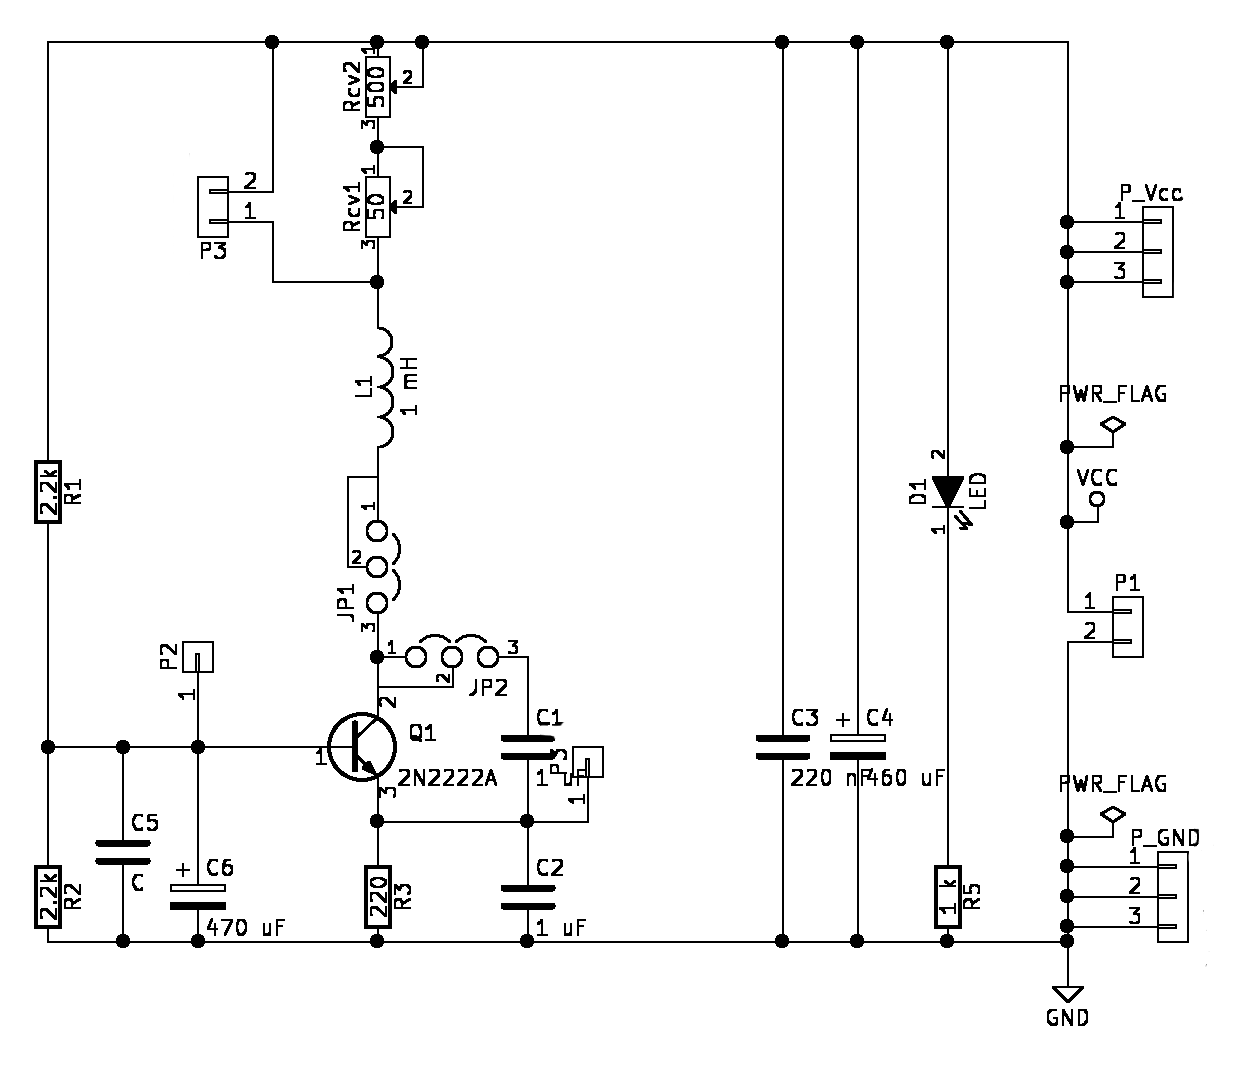
\includegraphics[width=0.45\textwidth]{p6/p/colp_schem_real.png} }
\caption{Електрична схема реального генератора Колпітца, яка була використана в даній роботі}
\label{atu:f:colp_schem_real}
\end{figure}

Впроваджену нову математичну модель,
яка враховує більше нелінійних властивостей
BJT транзистора, та різних режимів роботи.


Створено систему для отримання даних з використанням мікроконтролеру STM32F746 та пристроїв сполучення.
За ії використанням отримано дані з реального
генератора, За допомогою програмного комплексу ``qontrol'',
який описано у розділі 3, перевірити адекватність як
нової моделі генератора,
так і працездатність створеної для неї системи ідентифікації.

Розглянуто групу можливих критеріїв (рис.~\ref{atu:f:colp_q_cml}),
обрано критерій $q_{xz}$
та зроблено порівняльний аналіз цього критерію
для моделі та об'єкту (рис.~\ref{atu:f:colp_bjt_q-p_Rc_q}).

\begin{figure}[htb!]
\begin{center}
  ~ \hfill
  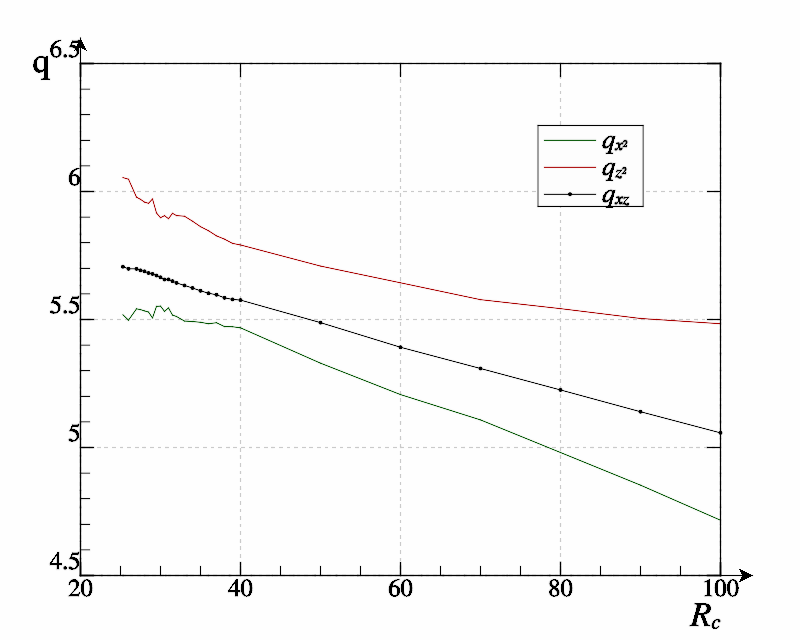
\includegraphics[width=0.42\textwidth]{p6/p/colp_read_q-p_Rc_q.png}
  \hfill
  \includegraphics[width=0.42\textwidth]{p6/p/colp_q_cml.png}
  \hfill ~
\end{center}
\vspace{-2.0ex}
\parbox[t]{0.45\textwidth}{
  \caption{Залежності значень критеріїв ідентифікації для моделі системи Колпітца}
  \label{atu:f:colp_bjt_q-p_Rc_q}
}
\hfill
\parbox[t]{0.45\textwidth}{
  \caption{Порівняння залежностей значень критерію ідентифікації $q_{xz}$ реального генератора Колпітца з моделлю}
  \label{atu:f:colp_q_cml}
}
\end{figure}

На підставі обраного критерію та групи методів ql3rlWvnAAW створено систему ідентифікації,
проведено 4 реальних експерименти зі змінним параметром $R_c$,
та проведено ідентифікацію~(рис.~\ref{atu:f:colp_r_id_1}).

\begin{figure}[htb!]
  \centerline{
    ~ \hfill
    \includegraphics[width=0.42\textwidth]{p6/p/r/colp_real_id-p_t_pi_ql3rlWvnAAW_real_d_0_xl.png}
    \hfill
    \includegraphics[width=0.42\textwidth]{p6/p/r/colp_real_id-p_t_p_ql3rlWvnAAW_real_d_0_xl.png}
    \hfill ~
  }
  \vspace{-1.5ex}
  \begin{center}
    ~ \hfill a \hfill\hfill b \hfill ~
  \end{center}
  \vspace{-2.5ex}
  \caption{Процес ідентифікації параметра $R_c$ реального генератора Колпітца:
  динаміка агентів (a) і різні методи визначення $p_\mathrm{id}$ (b)}
  \label{atu:f:colp_r_id_1}
\end{figure}

Результати ідентифікації продемонстрували, що метод ql3rlWvnAAW
при обробці реальних даних забезпечує як відповідність отриманих значень параметра $R_c$,
так і непогану швидкодію.



\textbf{У шостому розділі}
запропоновано модель
системи зв'язаних релаксаційних генераторів (``relax3d''),
які проявляють хаотичну динаміку при певних умовах.
Релаксаційні генератори, прямо або побічно, набули широкого поширення в схемотехніці.
Основними параметрами схем з релаксаційним генераторами є напруги включення
$V\Tidx{on}$ і виключення $V \Tidx{off}$ переключающего елементу,
напруга живлення $V\Tidx{cc}$, ємність конденсатора $C$, опору ланцюгів
зарядки $R\Tidx{ch}$ і розрядки $R\Tidx {dis}$.

Пропонований хаотичний генератор являє собою систему з трьох релаксаційних
генераторів. Елемент, що перемикає, в кожному з них реалізований на парі
компліментарних транзисторів~(рис.~\ref{atu:f:relax3d_schem}).
Параметр, що підлягає ідентифікації, було обрано $R_b$,
так як саме він контролює взаємодію між релаксаційними елементами.

% системи з трьох пов'язаних релаксаційних генераторів на парі компліментарних транзисторів

\begin{figure}[htb!]
  \centerline{\includegraphics[width=0.55\textwidth]{p7/p/relax3d_schem.png} }
  \caption{Електрична схема системи з трьох пов'язаних релаксаційних генераторів на парі компліментарних транзисторів}
  \label{atu:f:relax3d_schem}
\end{figure}


Створено дві схеми,
які реалізовують запропоновану динаміку, та відрізняються
засобом реалізації релаксаційних елементів.
Для отримання результатів використано мікроконтролерну систему,
яка була описана у попередньому розділі.

При певних значення $R_b$ зв'язок між релаксаційним елементами стає сильнішим,
і при цьому можлива ситуація, коли
процес заряду одного елемента настільки уповільнює момент перемикання іншого,
що це уповільнення впливає на всі елементи. Виникає стан ``гонки'', коли
перший елемент, що перейшов у режим зарядки істотно сповільнює перемикання другого. Таким
чином, виникає точка біфуркації, коли малі зміни в початковому стані системи
призводять до істотних змін в подальшій динаміці, що може призводити до
хаотичної поведінки.

При цьому спектр системи має щільні ділянки, підтверджуючи хаотичність
поведінки (рис.~\ref{atu:f:relax3d_f_08}, a). Аттрактор системи
(рис.~\ref{atu:f:relax3d_f_08}, b), навпаки, менш щільно заповнює
доступний простір.

\begin{figure}[htb!]
  \centerline{
    ~ \hfill
    \includegraphics[width=0.40\textwidth]{p7/p/relax3d_f_08_xl.png}
    ~
    \includegraphics[width=0.40\textwidth]{p7/p/relax3d_v1v2v3_08.png}
    \hfill ~
  }
  \vspace{-1.5ex}
  \begin{center}
    ~ \hfill a \hfill\hfill b \hfill ~
  \end{center}
  \vspace{-2.5ex}
  \caption{Спектр $V_b(t)$ (a) та аттрактор (b) для системи ``relax3d'' при $R_b=\SI{34.0}{\kilo\ohm}$ }
  \label{atu:f:relax3d_f_08}
\end{figure}

Модель системи пов'язаних релаксаційних генераторів можна представити в наступному вигляді:
%
\begin{equation}
  \begin{cases}
    V_b = V_{cc} - R_b ( I_1 + I_2 + I_3 ), \\
      C_1 \dot{V}_1 = \frac{V_b-V_1}{R_{v1}} - \frac{V_1}{R_1} \mathrm{On}_1() - I_{1,\mathrm{leak}}(V_1), \\
      C_2 \dot{V}_2 = \frac{V_b-V_2}{R_{v2}} - \frac{V_2}{R_2} \mathrm{On}_2() - I_{2,\mathrm{leak}}(V_2), \\
      C_3 \dot{V}_3 = \frac{V_b-V_3}{R_{v3}} - \frac{V_3}{R_3} \mathrm{On}_3() - I_{3,\mathrm{leak}}(V_3), \\
      I_i = \frac{V_b-V_i}{R_{vi}}.
  \end{cases}.
    \label{atu:eq:relax3}
\end{equation}
%
де:
$R_b$ --- опір в ланцюзі живлення (ідентифікований параметр),
$C_i$ --- ємності кожного з релаксаційних генераторів,
$R_{vi}$ --- опори зарядки релаксаційних генераторів,
$R_{i}$ --- опори зарядки релаксаційних генераторів,
$I_{i,\mathrm{leak}}$ --- струми витоку.
Функції $\mathrm{On}_i()$ визначають моменти спрацьовування переключаючих
елементів, і з огляду на їх релейно-гістерезісний вид задаються алгоритмічно.
Визначальними параметрами при цьому є
$V_{\mathrm{on},i}$, $V_{\mathrm{off},i}$.


Розглянуто декілька критеріїв (рис.~\ref{atu:f:relax3d_q}), та обрано критерій $q_{rv}$:
%
\begin{equation}
  q_{rv} = \frac{\overline{V_1+V_2+V_3}}{\overline{V_b}}.
  \label{atu:eq:q_rv_relax}
\end{equation}

\begin{figure}[htb!]
  \vspace{-1.6ex}
  \centerline{\includegraphics[width=0.46\textwidth]{p7/p/relax3d_read_q-p_q1_xl.png} }
  \vspace{-1.2ex}
  \caption{Залежності для розглянутих критеріїв ідентифікації для системи
  релаксаційних генераторів на парі компліментарних транзисторів.
  Щільні лінії відповідають об'екту, інші --- моделі}
  \label{atu:f:relax3d_q}
\end{figure}

Для системи ``relax3d'' було проведено 3 експерименти,
кожен з яких полягав в отриманні даних
($V_b(t)$, $V_1(t)$, $V_2(t)$, $V_3(t)$)
з реального генератора, з подальшим моделюванням процесу ідентифікації в
програмі ``qontrol''.
Результати моделювання процесу ідентифікації в першому експерименті
(рис.~\ref{atu:f:relax3d_id_1}) показують, що запропонована система
ідентифікації виявилася працездатною.

\begin{figure}[htb!]
  \centerline{
    ~ \hfill
    \includegraphics[width=0.45\textwidth]{p7/p/relax3d_read_id2-p_p_00_xl.png}
    \hfill
    \includegraphics[width=0.45\textwidth]{p7/p/relax3d_read_id2-p_pp_00_xl.png}
    \hfill ~
  }
  \vspace{-1.7ex}
  \begin{center}
    ~ \hfill a \hfill\hfill b \hfill ~
  \end{center}
  \vspace{-2.7ex}
  \caption{Процес ідентифікації системи ``relax3d'':
  динаміка агентів (a) і різні методи визначення $p_\mathrm{id}$ (b)}
  \label{atu:f:relax3d_id_1}
\end{figure}

Також досліджено вплив параметрів системи ідентифікації на похибки ідентифікації.
Підтверджена можливість використання широкого спектру цих параметрів.



\xsect{ВИСНОВКИ}

У роботі вирішена науково-технічна проблема ідентифікації параметрів складних технічних
систем у режимі хаотичної динаміки
з метою забезпечення їх керованої поведінки. При цьому:

\begin{itemize}

  \item
    створено нові критерії ідентифікації, які, на відміну від тих, що
    існують, придатні для аналізу стану та динаміки
    хаотичних систем, що створить фізично зумовлене обґрунтування працездатності систем
    ідентифікації;

  \item
    створено новий клас систем ідентифікації у межах
    адаптивно-пошуковой парадигми,
    які за рахунок використання колективної динаміки
    ансамблю пошукових агентів забезпечують
    кращу швидкість ідентифікації без істотного впливу на похибку ідентифікації;

  \item
    проведена перевірка працездатності запропонованих методів
    на прикладах як відомих систем хаотичної динаміки,
    так і на декількох інших динамічних систем, які проявляють
    складну та хаотичну динаміку;

  \item
   визначено, що системи з сухим тертям з точки зору задачі ідентифікації
   при певних  умовах функціонування
   мають властивості, що поєднують їх з системами хаотичної динаміки;

 \item
  створено програмне забезпечення, придатне для моделювання як систем
  хаотичної динаміки, так і систем мультиагентної ідентифікації;

  \item
  проведено як комп'ютерне моделювання процесів ідентифікації систем
  хаотичної динаміки, так і фізичне моделювання таких, що підтверджує адекватність
  побудованих моделей.


\end{itemize}



\nocite{*}

\xsect{Список опублікованих праць за темою дисертації}

\xxxsect{Статті у виданнях, що включені до міжнародних наукометричних баз:}

\printbibliography[heading=none, keyword=scimetr]


\xxxsect{Статті у наукових фахових виданнях:}

\printbibliography[heading=none, keyword=vak]

\xxxsect{Статті в закордонних виданнях:}

\printbibliography[heading=none, keyword=foreign]

\xxxsect{Матеріали наукових конференцій:}

\printbibliography[heading=none, keyword=confer]



\xsect{АННОТАЦИЯ}

\textbf{\dissauthorRu}
\textbf{\booknameRu}
\textbf{--- На правах рукописи.}

Диссертация на соискание ученой степени
доктора
\dissScopeRu\ {}
по специальности
\dissSpecId\ --- <<\dissSpecRu>>.
\institutionRu, \belongRu, \cityRu, \bookyear.


Ключевые слова:
хаотические системы,
критерии идентификации,
поисковый агент,
координатор поиска,
ансамблевые методы поисковой идентификации.


\xsect{АНОТАЦІЯ}

\textbf{\dissauthorUa}
\textbf{\booknameUa}
\textbf{--- На правах рукопису.}

Дисертація на здобуття наукового ступеня
доктора
\dissScopeUa\ {}
за спеціальністю
\dissSpecId\ --- <<\dissSpecUa>>.
\institutionUa, \belongUa, \cityUa, \bookyear.


Робота присвячена актуальній науково-технічній проблемі
ідентифікації параметрів складних технічних систем у режимі хаотичної динаміки.
Нелінійні динамічні системи, розповсюджені в сучасних технологічних і
природних процесах можуть проявляти хаотичні властивості в своїй динаміці.
Існуючи системи ідентифікації нелінійних динамічних об'єктів практично не
здатні функціонувати у таких умовах.

Ключові слова:
хаотичні системи,
критерії ідентифікації,
пошуковий агент,
координатор пошуку,
ансамблеві методи пошукової ідентифікації.

\xsect{ABSTRACT}

\textbf{\dissauthorEn}
\textbf{\booknameEn}.
\textbf{--- As Manuscript.}

Thesis for the degree of Doctor of Technical Science in Specialization
\dissSpecId\ --- <<\dissSpecEn>>.
\institutionEn, \belongEn, \cityEn, \bookyear.

The dissertation is devoted to

Keywords:
chaotic systems,
identification criteria,
searching agent,
searching coordinator,
ensemble methods of the searching indetification.

\clearpage

{~}
\vfill

\begin{center}


Підписано до друку xx.xx.\bookyear~р.

Формат $60 \times 84/16$  Папір друкарський. Ум. др.арк.~2

Друк різограф. Замовлення \No 02/17. Наклад --- 100 прим.

% ДНВП <<Системні технології>>

49006, Дніпро, пр.~Гагаріна,~4

st@nmetau.edu.ua

\end{center}

\vfill


\end{document}

